
\chapter{Deep Learning}\label{chap:deep}\label{part:deep}
%\noindent Use the template \emph{part.tex} together with the document class SVMono (monograph-type books) or SVMult (edited books) to style your part title page and, if desired, a short introductory text (maximum one page) on its verso page.

This chapter is focused on a specific topic in modern machine learning, i.e., deep learning. First of all, we introduce a few fundamental aspects, including perceptron and why we need multi-layer structures, how the convolutional neural networks extract features layer by layer, the back-propagation learning algorithm, and the functional layers of convolutional neural networks. Then, we will focus on the safety and security vulnerabilities of deep learning, explaining uncertainty estimation, adversarial attack on the robustness, poisoning attack, model stealing, membership inference and model inversion. 
%
Unlike traditional machine learning models that we discussed in the previous chapters where the structure or the training algorithm of a machine learning model may be considered for the design of the attacks, most attacks  for deep learning do not consider the internal structure of a deep learning model, although the gradient may be used in some cases. These black-box or grey-box attacks suggest that many of the attack algorithms for deep learning may also be applicable to traditional machine learning models, which explains why we frequently refer to algorithms in the chapter when discussing safety threads for traditional machine learning models. 

%Nevertheless,  algorithms in chapter are heuristic, i.e., they are able to discover the safety threads but cannot confirm the in-existence of them. 



%\chapter{Safety of Deep Learning}\label{chap:deep}



%\newpage
\section{Perceptron}\label{sec:perceptron}


\subsection*{Biological vs Artificial Neurons}

A human brain contains billions of neurons, which -- as shown in Figure~\ref{fig:bioneuron} -- are inter-connected nerve cells that are involved in processing and transmitting chemical and electrical signals. Neurons use 
dendrites as branches to receive information from other neurons. The received information is processed by 
the cell body or Soma. A neuron sends information to other neurons through a cable -- called axon -- and the synapse which connects an axon with other neurons' dendrites. 

\begin{figure}[!htbp]
    \centering
    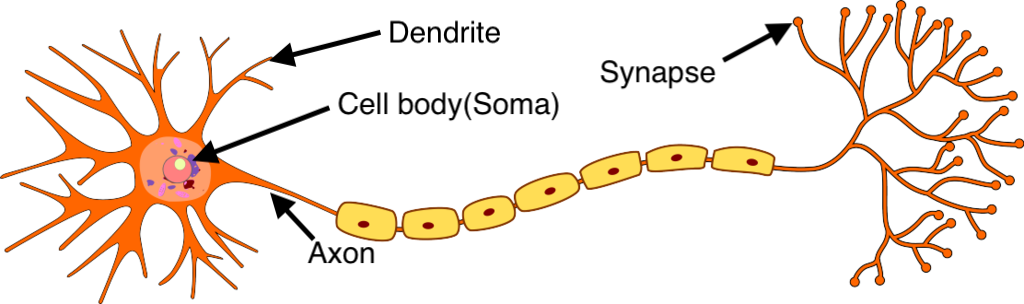
\includegraphics[width=0.7\textwidth]{images/deepLearning/Perceptron/biologicalNeuron.png}
    \caption{Biological Neuron (from Wikipedia)}
    \label{fig:bioneuron}
\end{figure}

In 1943, Warren McCullock and Walter Pitts published a simplified brain cell,  called McCullock-Pitts (MCP) neuron. As shown in Figure~\ref{fig:artneuron}, an artificial neuron represents a nerve cell as a simple logic gate with binary outputs. It takes inputs, weighs them separately, sums them up, and passes this sum through a nonlinear function to produce output. 

\begin{figure}[!htbp]
    \centering
    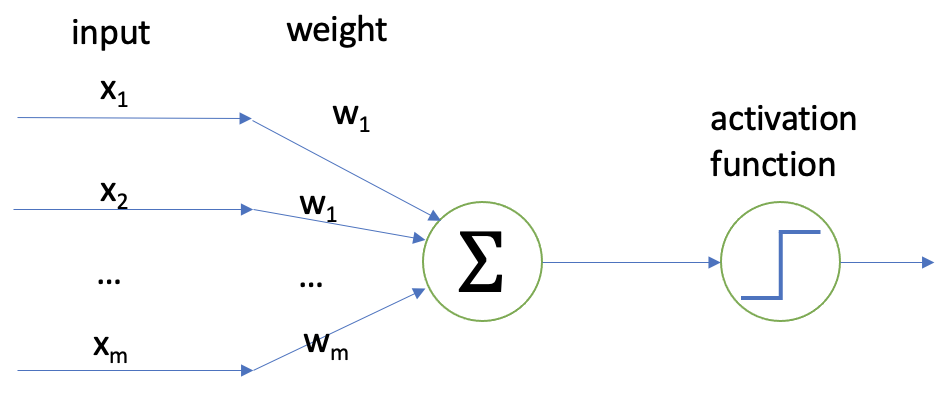
\includegraphics[width=0.6\textwidth]{images/deepLearning/Perceptron/artificialNeuron2.png}
    \caption{Artificial Neuron}
    \label{fig:artneuron}
\end{figure}

Table~\ref{tab:bioartneurons} is a brief conceptual mapping between biological and artificial neurons. 

\begin{table}[!htbp]
    \centering
    \begin{tabular}{|l|l|}
    \hline
       Biological Neuron  &  Artificial Neuron \\
       \hline
        dentrites & input \\
        cell body (soma) & node \\
        axon & output \\
        synapse & weights \\ 
        \hline
    \end{tabular}
    \caption{Mapping of Concepts between Biological and Artificial Neurons}
    \label{tab:bioartneurons}
\end{table}

\subsection*{Learning Algorithm of Perceptron}

A perceptron is an artificial neuron that does certain computations (such as detect features or execute business intelligence) on the input data. 
Perceptron was introduced by Frank Rosenblatt in 1957, when he proposed a perceptron learning rule based on the original MCP neuron. In July 1958, an IBM 704 – a 5-ton computer with the size of a room – was fed a series of punch cards. After 50 trials, the computer taught itself to distinguish cards marked on the left from cards marked on the right \cite{cornell2019}. It was a demonstration of the ``perceptron'', and was ``the first machine which is capable of having an original idea,'' according to its creator, Frank Rosenblatt. 


A perceptron learning algorithm is a  supervised learning of binary classifiers. The binary classifier  processes an input $\textbf{x}=(x_1,...,x_m)$ as follows: 
\begin{enumerate}
    \item Use one weight $w_i$ per feature $X_i$;  
    \item Multiply weights $w_i$ with the  respective input features $x_i$ of $\textbf{x}$, and add bias $w_0$; 
    \item If the result is greater than a pre-specified threshold, return 1. Otherwise, return 0. 
\end{enumerate}

The weights $w_1,...,w_m$ and bias $w_0$ of the binary classifier need to be learned. Given a set $D$ of training instances, the learning algorithm proceeds as follows: 

\begin{itemize}
    \item Initialize weights randomly,
    \item Take one sample $(\textbf{x}_i,y_i)\in D$ and make a prediction ${\hat y}_i$,  
    \item For erroneous predictions,  update weights with the following rules: 
    \begin{itemize}
        \item If the output is ${\hat y}_i=0$ but the label is $y_i=1$, increase the weights. 
       
        \item If the output is ${\hat y}_i=1$ but the label is $y_i=0$, decrease the weights.
    \end{itemize}
    that is, we let 
     \begin{equation}
            w_i=w_i+\Delta w_i \text{~~~~ such that ~~~~} \Delta w_i = \eta(y_i-{\hat y}_i) \textbf{x}_i
        \end{equation}
    where $\eta \ll 1$ is a constant representing the learning rate.
\end{itemize}

\subsection{Expressivity of Perceptron}\label{sec:perceptronexpressivity}

While simple, perceptron is the foundation of modern deep learning, which  uses a network of perceptrons where there are multiple layers and there are multiple neurons per layer.  
%
Why do we need a multi-layer perceptron (MLP) instead of just a single perceptron? This is a question related to the expressivity of a single perceptron. Actually, as we will show below, a single perceptron can express some useful functions but cannot do well for others. 

\subsection*{Linearly separable function} 

As perceptron is a linear classifier, it is able to work well on all linearly separable datasets, i.e., classify instances that can be separated with a linear function. 

\begin{example}
\begin{table}[!htbp]
    \centering
    \begin{tabular}{|c|c||c|}
    \hline
     $X_1$  &  $X_2$   &  \textbf{y} \\
     \hline
      0     & 0  & 0 \\
      0 & 1 & 0 \\
      1 & 0 & 0 \\
      1 & 1 & 1 \\
      \hline
    \end{tabular}
    \caption{Truth table for logic $\land$ (And)}
    \label{tab:truthtableand}
\end{table}
Table~\ref{tab:truthtableand} presents an example dataset of four instances for the logic operator $\land$. Actually, we generalise the logic operator $\land $ to the following function. 
\begin{equation}
    f_\land(x_1,x_2) = 
    \begin{cases}
    1 & \text{ if } x_1 > 0.5 \text{ and } x_2 > 0.5 \\
    0 & \text{otherwise}
    \end{cases}
\end{equation}

In Figure~\ref{fig:logicand}, we use squares to represent 0 and triangles to represent 1. By learning a perceptron, it is possible to get a linear separation function as exhibited in the figure. We use different colors to denote different areas in which the instances should be classified accordingly. In Figure~\ref{fig:logicand}, we also generate a random sample of 100 instances and use the learned perceptron to predict the instances with different colors (with an accuracy close to 1.0).  

\begin{figure}[!htbp]
    \centering
    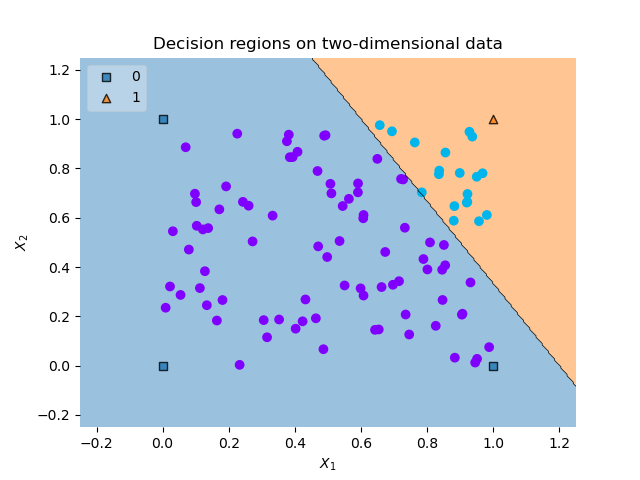
\includegraphics[width=0.7\textwidth]{images/deepLearning/Perceptron/logicand.png}
    \caption{Visualisation of a perceptron learned from the data instances in Table~\ref{tab:truthtableand}}
    \label{fig:logicand}
\end{figure}
\end{example}

\begin{example}
The other example is as shown in  Table~\ref{tab:truthtableor}, presenting  an example dataset of four instances for the logic operator $\lor$. Actually, we generalise the logic operator $\lor $ to the following function. 
\begin{equation}
    f_\lor(x_1,x_2) = 
    \begin{cases}
    1 & \text{ if } x_1 > 0.5 \text{ or } x_2 > 0.5 \\
    0 & \text{otherwise}
    \end{cases}
\end{equation}

\begin{table}[!htbp]
    \centering
    \begin{tabular}{|c|c||c|}
    \hline
     $X_1$  &  $X_2$   &  \textbf{y} \\
     \hline
      0     & 0  & 0 \\
      0 & 1 & 1 \\
      1 & 0 & 1 \\
      1 & 1 & 1 \\
      \hline
    \end{tabular}
    \caption{Truth table for logic $\lor$ (Or)}
    \label{tab:truthtableor}
\end{table}
Figure~\ref{fig:logicor} presents the visualisation of the learned perceptron. We can see that,  the separating line is different from that of Figure~\ref{fig:logicand}. The separating lines in both figures are able to separate the data very well (with accuracy close to 1.0). 
\begin{figure}[!htbp]
    \centering
    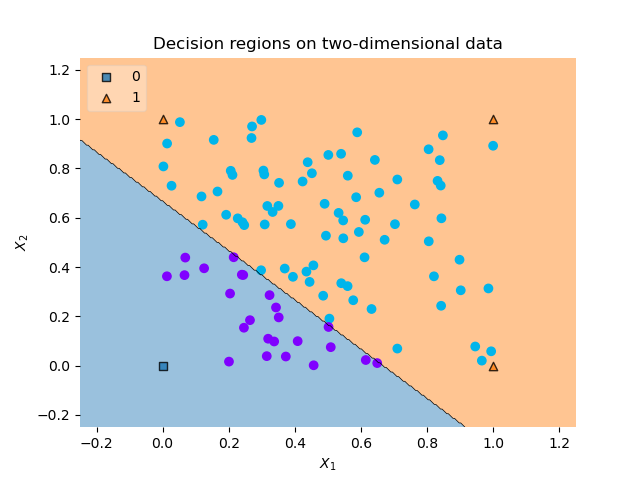
\includegraphics[width=0.7\textwidth]{images/deepLearning/Perceptron/logicor.png}
    \caption{Visualisation of a perceptron learned from the data instances in Table~\ref{tab:truthtableor}}
    \label{fig:logicor}
\end{figure}
\end{example}

The above examples are all based on a 2-dimensional dataset. The learned perceptrons are actually a line on the 2-dimensional space. When the dataset is $d$-dimensional, the perceptron is a $d$-dimensional hyper-plane. 

\subsection*{Linearly inseparable function}

Unfortunately, not all datasets are linearly separable. 

\begin{example}\label{example:xor}
%For example, 
Table~\ref{tab:truthtablexor} is a dataset of four instances, which is generated from the following function:  
\begin{equation}
    f_\oplus(x_1,x_2) = 
    \begin{cases}
    1 & \text{ if } x_1 > 0.5 \text{ and } x_2 < 0.5 \\
    1 & \text{ if } x_1 < 0.5 \text{ and } x_2 > 0.5 \\
    0 & \text{otherwise}
    \end{cases}
\end{equation}
\begin{table}[!htbp]
    \centering
    \begin{tabular}{|c|c||c|}
    \hline
     $X_1$  &  $X_2$   &  \textbf{y} \\
     \hline
      0     & 0  & 0 \\
      0 & 1 & 1 \\
      1 & 0 & 1 \\
      1 & 1 & 0 \\
      \hline
    \end{tabular}
    \caption{Truth table for logic $\oplus$ (XOR)}
    \label{tab:truthtablexor}
\end{table}
While we can still apply perceptron, the learned perceptron cannot reach high accuracy ($\sim$ 0.5 accuracy). 
\end{example}

Therefore, this example shows that the perceptron in itself does not have sufficient expressiveness to work with complex functions. This contributes as the reason why we have to consider multiple layers and more neurons.  

\subsection{Multi-layer Perceptron} 

To deal with the XOR problem, a two-layer perceptron as shown in Figure~\ref{fig:twolayerxor} has been suggested. 

\begin{figure}[!htbp]
    \centering
    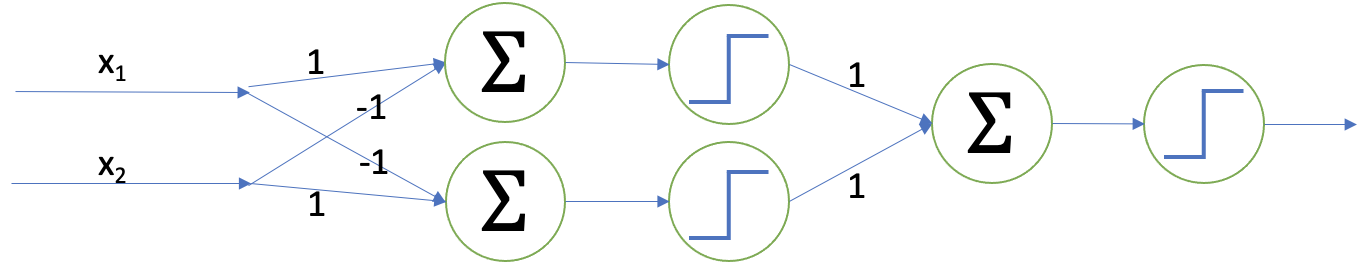
\includegraphics[width=0.7\textwidth]{images/deepLearning/Perceptron/minsky.png}
    \caption{A two-layer perceptron to solve XOR problem}
    \label{fig:twolayerxor}
\end{figure}
where the activation function is $ReLU(x) = \max(0,x)$. 

If written in the matrix form, we have the following expressions for the training data, which shows that the above two-layer perceptron perfectly classifies the training data. 

\begin{equation}
\begin{blockarray}{cc}
\begin{block}{(cc)}
   0 & 0 \\
   0 & 1 \\
   1 & 0 \\
   1 & 1 \\
\end{block}
\end{blockarray}
\times 
\begin{blockarray}{cc}
\begin{block}{(cc)}
   1 & 1 \\
   -1 & 1 \\
\end{block}
\end{blockarray}
=
\begin{blockarray}{cc}
\begin{block}{(cc)}
   0 & 0 \\
   -1 & -1 \\
   1 & -1 \\
   0 & 0 \\
\end{block}
\end{blockarray}
\text{~~ and ~~} ReLU
\begin{blockarray}{cc}
\begin{block}{(cc)}
   0 & 0 \\
   -1 & -1 \\
   1 & -1 \\
   0 & 0 \\
\end{block}
\end{blockarray} = 
\begin{blockarray}{cc}
\begin{block}{(cc)}
   0 & 0 \\
   0 & 1 \\
   1 & 0 \\
   0 & 0 \\
\end{block}
\end{blockarray}
\label{equ:twolayerperceptron}
\end{equation}

\begin{equation}
\begin{blockarray}{cc}
\begin{block}{(cc)}
   0 & 0 \\
   0 & 1 \\
   1 & 0 \\
   0 & 0 \\
\end{block}
\end{blockarray} \times 
\begin{blockarray}{c}
\begin{block}{(c)}
   1  \\
   1  \\
\end{block}
\end{blockarray}
=
\begin{blockarray}{c}
\begin{block}{(c)}
   0  \\
   1  \\
   1  \\
   0  \\
\end{block}
\end{blockarray}
\text{~~ and ~~} 
ReLU
\begin{blockarray}{c}
\begin{block}{(c)}
   0  \\
   1  \\
   1  \\
   0  \\
\end{block}
\end{blockarray} = 
\begin{blockarray}{c}
\begin{block}{(c)}
   0  \\
   1  \\
   1  \\
   0  \\
\end{block}
\end{blockarray}
\label{equ:twolayerperceptron}
\end{equation}

\subsection{Practice}


\subsection*{Train a perceptron}

First of all, we load and prepare datasets. 

\begin{lstlisting}[language=Python]
from sklearn import datasets
dataset = datasets.load_digits()
X = dataset.data
y = dataset.target

observations = len(X)
features = len(dataset.feature_names)
classes = len(dataset.target_names)
print("Number of Observations: " + str(observations))
print("Number of Features: " + str(features))
print("Number of Classes: " + str(classes))

from sklearn.model_selection import train_test_split
X_train, X_test, y_train, y_test = train_test_split(X, y, test_size=0.20)
\end{lstlisting}

Then, we can call \textbf{sklearn}'s library function to train a perceptron model. 

\begin{lstlisting}[language=Python]
from sklearn.linear_model import Perceptron

clf = Perceptron(tol=1e-3, random_state=0)
clf.fit(X_train, y_train)
print("Training accuracy is %s"% clf.score(X_train,y_train))
print("Test accuracy is %s"% clf.score(X_test,y_test))

print("Labels of all instances:\n%s"%y_test)
y_pred = clf.predict(X_test)
print("Predictive outputs of all instances:\n%s"%y_pred)

from sklearn.metrics import classification_report, confusion_matrix
print("Confusion Matrix:\n%s"%confusion_matrix(y_test, y_pred))
print("Classification Report:\n%s"%classification_report(y_test, y_pred))
\end{lstlisting}


\subsection*{Display class regions for Boolean functions}

In the following, we present how to generate the visualisation as in Figure~\ref{fig:logicand} and Figure~\ref{fig:logicor}.
%
First of all, we install a package \textbf{mlxtend}. 

\begin{cmds}
pip3 install mlxtend
\end{cmds}

Then, we need to load the data instances $\textbf{X}=\{(0,0),(0,1),(1,0),(1,1)\}$ and their labels. Note that, in the below code, we use \textbf{logical\_and}. You are able to use others such as \textbf{logical\_or} and \textbf{logical\_xor}. 

\begin{lstlisting}[language=Python]
import numpy as np
# Loading data
X_train = np.array([[0.0,0.0],[0.0,1.0],[1.0,0.0],[1.0,1.0]])
y_train = np.array(np.logical_and(X_train[:, 0] > 0.5, X_train[:, 1] > 0.5), 
             dtype=int)
\end{lstlisting}

Once the data is loaded, we train a Perceptron, with initial parameters $\textbf{w}=(1.5,1.5)$. Note that, this is simply for the experiment, and it can be initialised to other values, or set as default by ignoring the parameter \textbf{coef\_init}. 

\begin{lstlisting}[language=Python]
# Training a classifier
from sklearn.linear_model import Perceptron
clf = Perceptron(tol=1e-3, random_state=0)
clf.fit(X_train, y_train, coef_init=np.array([[1.5],[1.5]]))
\end{lstlisting}

We can print the final learned weights. 

\begin{lstlisting}[language=Python]
print(clf.coef_)
\end{lstlisting}

Finally, we can plot the regions for the classes. 

\begin{lstlisting}[language=Python]
# Plotting decision regions
from mlxtend.plotting import plot_decision_regions
plot_decision_regions(X_train, y_train, clf=clf, legend=2)
\end{lstlisting}

We may also generate a set of random points and plot them. 

\begin{lstlisting}[language=Python]
# Plotting randomly generated points 
import matplotlib
import matplotlib.pyplot as plt
import random

n_sample = 100
X_test = np.array([[random.random() for i in range(2)] for j in range(n_sample)])
y_test = np.array(np.logical_and(X_test[:,0]>0.5,X_test[:,1]>0.5),dtype=int)
y_pred = clf.predict(X_test) 
print(clf.score(X_test,y_test))
colors = matplotlib.cm.rainbow(np.linspace(0, 1, 5))
plt.scatter(X_test[:, 0],X_test[:, 1],color=[colors[i] for i in y_pred])
\end{lstlisting}

\begin{lstlisting}[language=Python]
# Adding axes annotations
import matplotlib.pyplot as plt
plt.xlabel('X_1')
plt.ylabel('X_2')
plt.title('Decision regions on two-dimensional data')
plt.show()
\end{lstlisting}



%\newpage
\section{Functional View}

A deep neural network can be seen as a family of parametric, non-linear, and hierarchical representation learning functions. These learning functions are massively optimized with stochastic gradient descent (SGD) over some pre-specified objectives, such as the loss of a set of training instances. It is expected that, the learned functions will encode domain knowledge that is implicitly presented in the training instances. 


\subsection{Mappings between High-dimensional Spaces}

Consider a feed-forward network as shown in Figure~\ref{fig:feedforward}. Assume that it has $m+1$ layers, where Layer-0 is the input layer,  Layer-$m$ is the output layer, and Layer-1 to Layer-$(m-1)$ are the hidden layers. 

\begin{figure}[!htbp]
    \centering
    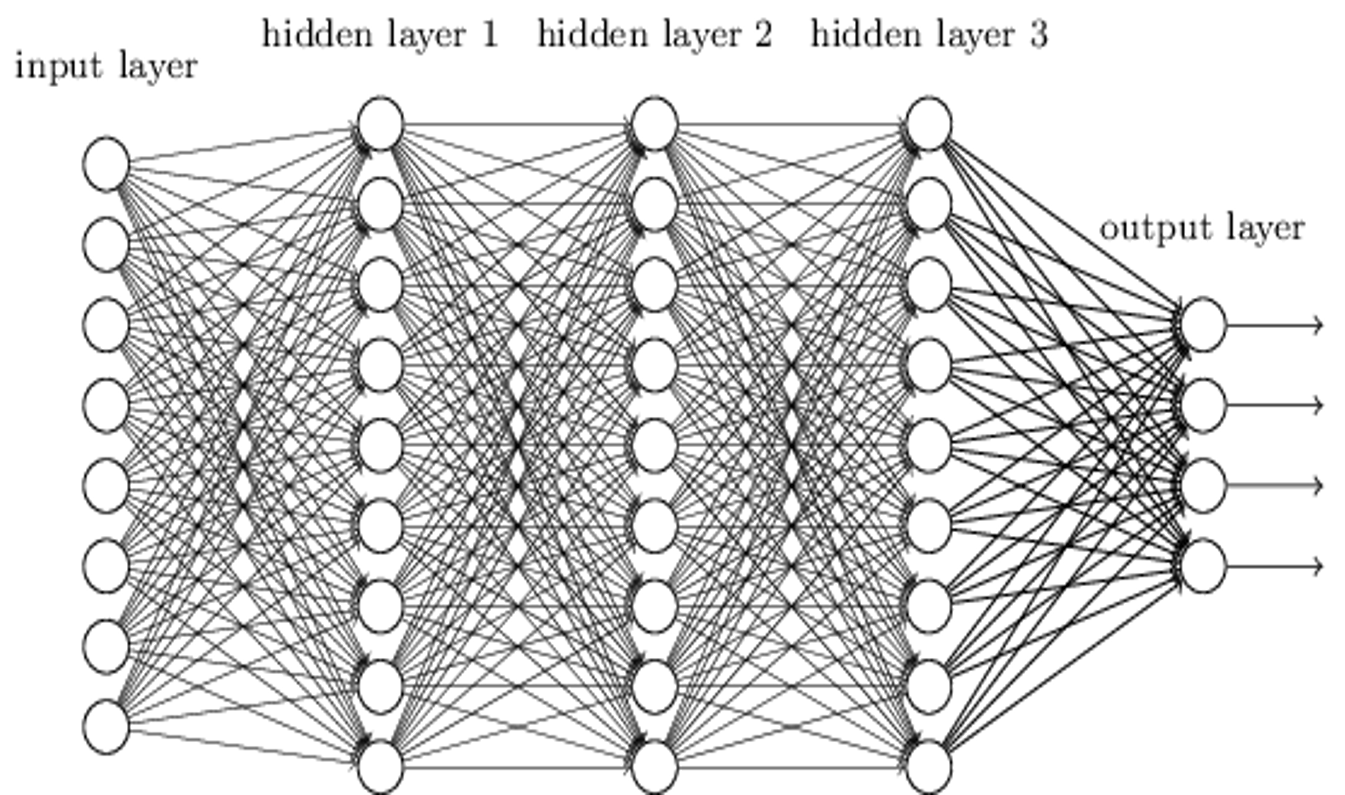
\includegraphics[width=0.6\textwidth]{images/deepLearning/functionalView/nn.png}
    \caption{A 5 layer feed-forward network}
    \label{fig:feedforward}
\end{figure}

Every layer is a function, so we have functions $f_1,...,f_{m}$, for hidden layers and output layer, and because every function is parameterised, we use $\textbf{W}=\{\textbf{W}_1,...,\textbf{W}_m\}$ to denote their parameters. Based on these, a neural network can be written in a functional way as follows. 

\begin{equation}
    f_{\textbf{W}}(\textbf{x};\textbf{W}_1,...,\textbf{W}_m) = f_m(f_{m-1}(... f_1(\textbf{x};\textbf{W}_1),\textbf{W}_{m-1});\textbf{W}_m)
\end{equation}
Alternatively, we may write 
\begin{equation}\label{equ:mappings}
\begin{array}{lclcl}
    f_{\textbf{W}}(\textbf{x}) & = & \textbf{v}_m & = &  f_{m}(\textbf{v}_{m-1};\textbf{W}_{m})\\
   && \textbf{v}_{m-1} & = & f_{m-1}(\textbf{v}_{m-2};\textbf{W}_{m-1}) \\
   && ...\\
   && \textbf{v}_{2} & = & f_{2}(\textbf{v}_{1};\textbf{W}_{2}) \\
   && \textbf{v}_{1} & = & f_{1}(\textbf{v}_{0};\textbf{W}_{1}) \\
\end{array}
\end{equation}
where $\textbf{v}_i$ is the output value of Layer-$i$. Note that, we have both $\textbf{v}_i$ and $\textbf{W}_i$ as vectors or matrices, because it is typical that there are many neurons per layer and the layer functions are parameterised with many parameters. 

Take a closer look at Equation (\ref{equ:mappings}), given a function $\textbf{v}_{i} = f_{i}(\textbf{v}_{i-1};\textbf{W}_{i})$, once the parameters $\textbf{W}_i$ are learned, it is a transformation from $\textbf{v}_{i-1}$ to $\textbf{v}_{i}$. Let each layer-$i$ have $k_i$ neurons, we have that  $\textbf{v}_{i-1}$ is a vector of $k_{i-1}$ entries and $\textbf{v}_{i}$ is a vector of $k_{i}$ entries. Therefore, the transformation can be seen as a mapping from high-dimensional space $\real^{k_{i-1}}$ to $\real^{k_{i}}$. Generalise this to the entire network, we have 
\begin{equation}
   \displaystyle \real^{k_0} \xmapsto{f_1} \real^{k_1} \xmapsto{f_2} ... \xmapsto{f_m} \real^{k_m}
\end{equation}
Note that, $k_0$ is the number of input features and $k_m$ is the number of class labels. 

\subsection*{Training Objective}

The training typically intends to get the best weights $\textbf{W}^*$ as follows. 
\begin{equation}
    \textbf{W}^* \leftarrow \argmin_{\textbf{W}} \sum_{(\textbf{x},{y})\in D} L(y,\textbf{v}_m)
\end{equation}
where $L(y,f_{\textbf{W}}(\textbf{x}))$ is typically a loss function measuring the gap between actual label $y$ with its current prediction $f_{\textbf{W}}(\textbf{x})$. 
However, the optimisation problem is highly dimensional and non-convex. Therefore, in most cases, the training ends up with an approximation $\hat{\textbf{W}}$. 

\subsection{Recurrent Neural Networks}

The above is mainly for feedforward neural networks (FNNs), which model a function $\dnnfunction:X\rightarrow Y$ that maps from input domain $X$ to output domain $Y$: given an input $x\in X$, it outputs the prediction $y\in Y$. For a sequence of inputs $x_1,\dots,x_n$, an FNN $\dnnfunction$ considers each input individually, that is, $\dnnfunction(x_i)$ is independent from $\dnnfunction(x_{i+1})$. 

%and is %usually 
%used to perform predictions based on an input $x\in X$, or recognise patterns in $x$. 
%For a sequence of inputs $x_1,...,x_n$, $\dnnfunction$ will handle them individually without considering  results from previous predictions, that is, the result of $\dnnfunction(x_i)$ is independent of the results of $\dnnfunction(x_j)$ when $j\neq i$. 

By contrast, a recurrent neural network (RNN) 
%are designed to handle sequential data. An RNN contains at least one recurrent layer
%, as depicted in Fig.~\ref{fig:recurrent}, 
%that 
processes 
an input sequence by iteratively taking inputs one by one. 
%sequential input.
%illustrates how a sequential input is handled by a recurrent layer by unfolding.
A recurrent layer can be modeled as a function 
$\rnnfunction:X'\times C\times Y' \rightarrow C\times Y'$
such that 
$\rnnfunction(x_t,c_{t-1},h_{t-1})=(c_t,h_t)$ for $t=1,...,n$, 
where $t$ denotes the $t$-th time step, $c_t$ is the cell state used to represent the intermediate memory and $h_{t}$ is the output of the $t$-th time step.  
More specifically, the recurrent layer takes three inputs: $x_t$ at the current time step, the prior memory state $c_{t-1}$ and the prior cell output $h_{t-1}$; consequently, it updates the current cell state $c_t$ and outputs current $h_{t}$.   
%Initially, we let $c_0$ and $h_0$ be 0-valued vectors. For a (finite) sequence of inputs $x_1,...,x_n$, this function $\rnnfunction$ is applied recursively on them. 
%For example, the popular long short-term memory (LSTM) layer can be represented with the following equations for time~$t$: 

RNNs differ from each other given their respective definitions, i.e., internal structures, of recurrent layer function $\rnnfunction$, of which long short-term memory (LSTM) in Equation (\ref{eq:lstm}) is the most popular and commonly used one. 
%
\begin{equation}
\label{eq:lstm}
\begin{array}{lcl}
f_t & = & \sigma(W_f\cdot [h_{t-1},x_t] + b_f) \\ 
i_t & = & \sigma(W_i\cdot [h_{t-1},x_t] + b_i) \\ 
c_t & = & f_t*c_{t-1} + i_t * \tanh(W_c\cdot [h_{t-1},x_t] + b_c)\\
o_t & = & \sigma(W_o\cdot [h_{t-1},x_t] + b_o) \\ 
h_t & = &  o_t * \tanh(c_t)
\end{array}
\end{equation}
%
such that $\sigma(x)\in [0,1]$ for any $x\in\real$, $\tanh$ is the hyperbolic tangent function such that $\tanh(x)\in [-1,1]$ for any $x\in\mathbb{R}$, $W_f,W_i,W_c,W_o$ are weight matrices, $b_f,b_i,b_c,b_o$ are bias vectors,  $f_t,i_t,o_t$ are internal gate variables, $h_t$ is the hidden state variable (utilising $o_t$), and $c_t$ is the cell state variable. For the connection with successive layers, we only take the last output $h_n$ as the output. For simplicity, when working with finite sequential data, we can also define a recurrent layer as $\rnnfunction:(X')^n\rightarrow Y'$, which takes, as input, a sequential data of length $n$ and returns the last output $h_n$. Figure~\ref{fig:Cell} presents an illustrative diagram for LSTM cell. 

\begin{figure}[!htbp]
    \centering
    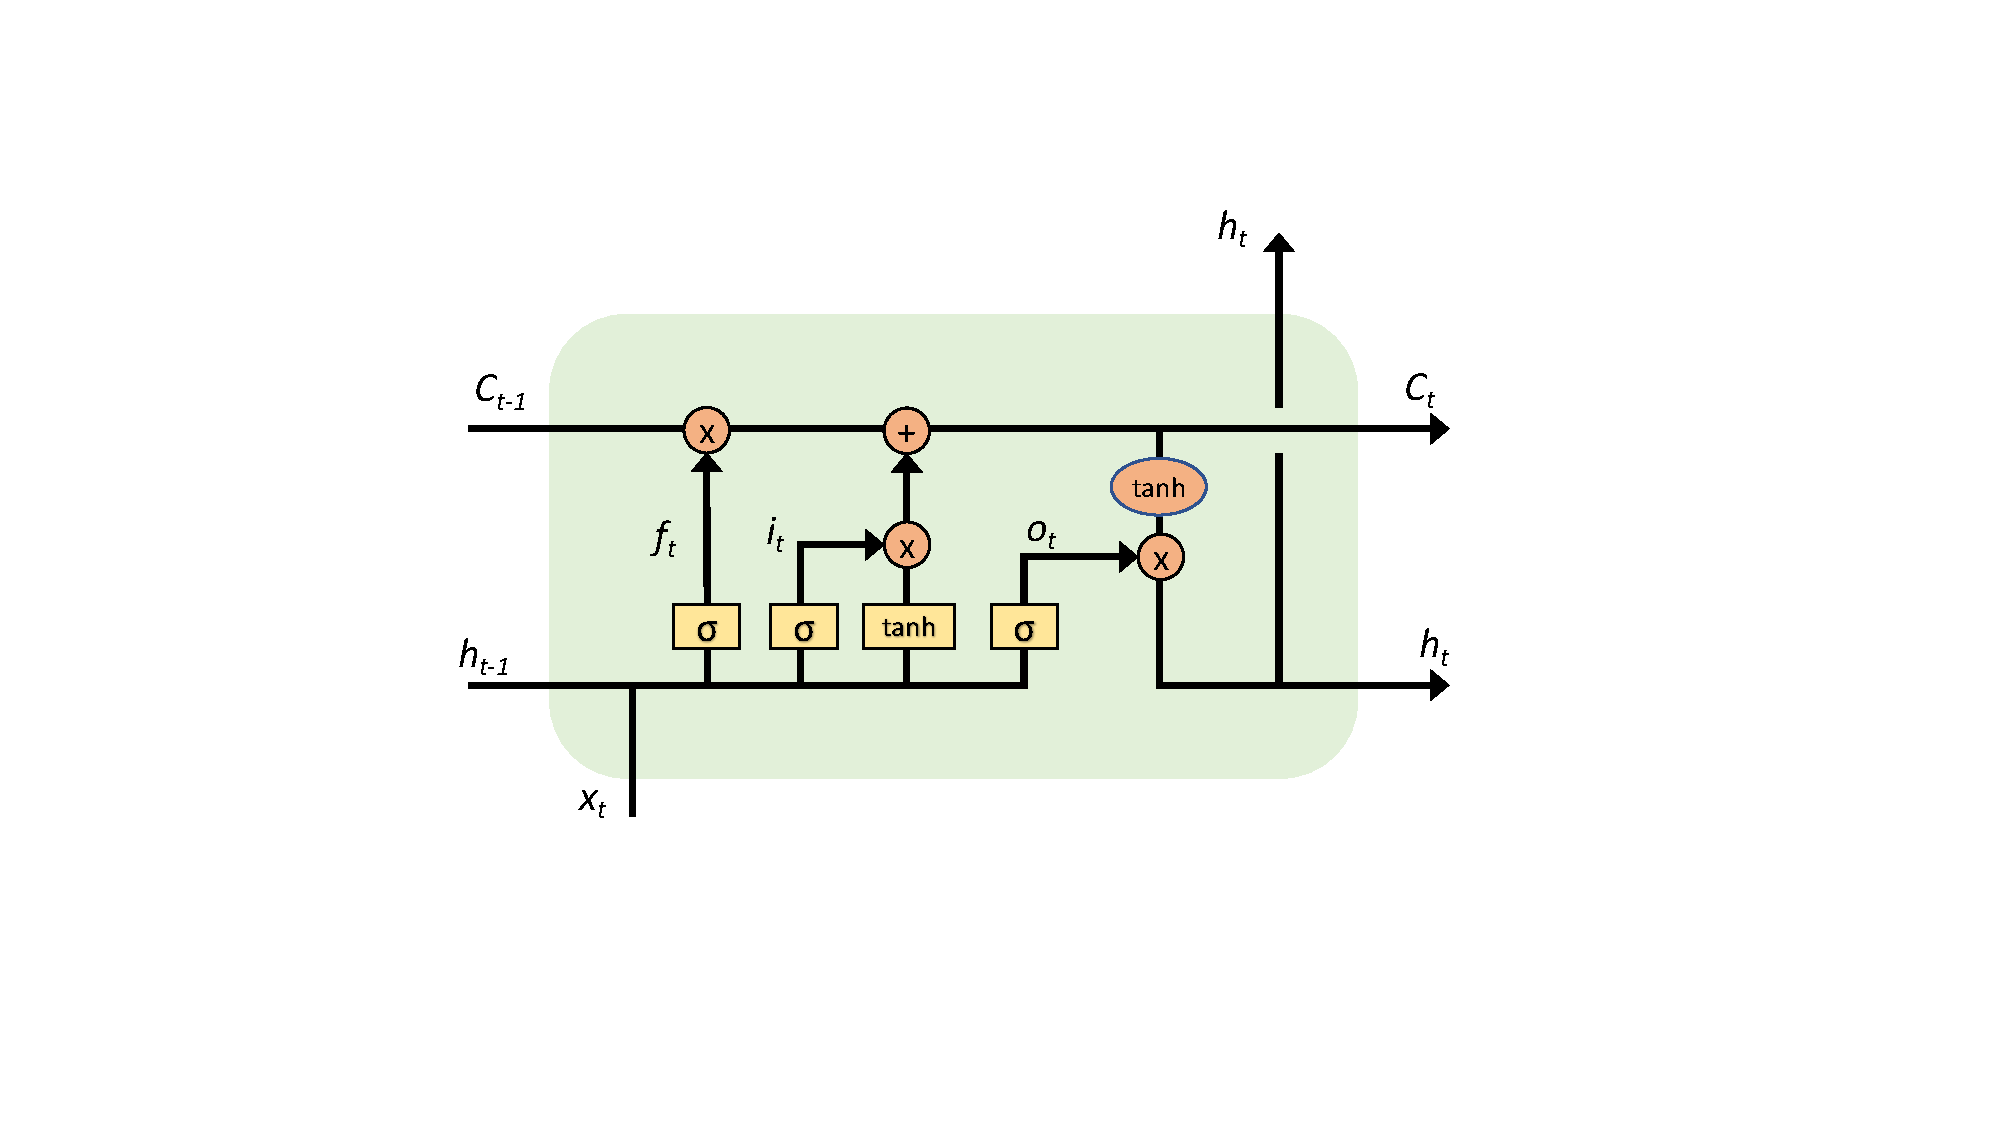
\includegraphics[width=0.65\linewidth]{images/deepLearning/functionalView/LSTM_cell.pdf}
    \caption{LSTM Cell}
    \label{fig:Cell}
\end{figure}


In LSTM, $\sigma$ is the sigmoid function and $\tanh$ is the hyperbolic tangent function; $W$ and $b$ represent the weight matrix and bias vector, respectively; $f_t,i_t,o_t$ are internal gate variables of the cell.
%Fig. \ref{fig:Cell} gives an diagrammatic illustration of an LSTM cell. 
In general, the recurrent layer (or LSTM layer) is connected to non-recurrent layers such as fully connected layers so that the cell output propagates further. We denote the remaining layers with a function $\dnnfunction_2:Y'\rightarrow Y$. Meanwhile, there can be feedforward layers connecting to the RNN layer, and we let it be another function $\dnnfunction_1:X\rightarrow X'$. As a result, the RNN model that accepts a sequence of inputs $x_1,\dots,x_n$ can be modeled as a function $\varphi$ such that 
%\begin{equation}
$\varphi(x_1...x_n) = \dnnfunction_2\cdot\rnnfunction(\prod_{i=1}^n \dnnfunction_1(x_i))$.
%\end{equation}
%
%
Normally, the recurrent layer is connected to non-RNN layers such as fully connected layers so that the output $h_n$ is processed further. We let the remaining layer be a function $\dnnfunction_2:Y'\rightarrow Y$. Moreover, there can be feedforward layers connecting to the RNN layer, and we let it be a function $\dnnfunction_1:X\rightarrow X'$. Then given a sequential input $x_1,...,x_n$, the RNN is a function $\varphi$ such that 
%



\subsection{Learning Representation and Features}\label{sec:representationlearning}

\subsection*{Raw digital representation}

Every instance has to be represented in a digital form. For example, the 8th instance in the \textbf{digits} dataset is an image of digit 8 as shown in Figure~\ref{fig:digit8}. 

\begin{figure}[!htbp]
    \centering
    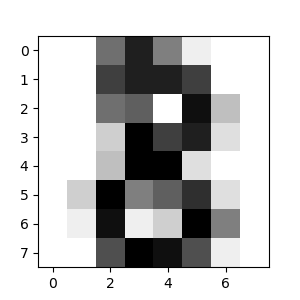
\includegraphics[width=0.2\textwidth]{images/deepLearning/functionalView/digit_8.png}
    \caption{A small image of digit 8}
    \label{fig:digit8}
\end{figure}

Actually, it is stored as a matrix as follows:  

\begin{equation}
\begin{blockarray}{cccccccc}
\begin{block}{(cccccccc)}
0 &   0 &   9 &  14 &   8 &   1 &   0 &   0 \\
0 &   0 &  12 &  14 &  14 &  12 &   0 &   0 \\
0 &   0 &   9 &  10 &   0 &  15 &   4 &   0 \\
0 &   0 &   3 &  16 &  12 &  14 &   2 &   0 \\
0 &   0 &   4 &  16 &  16 &   2 &   0 &   0 \\
0 &   3 &  16 &   8 &  10 &  13 &   2 &   0 \\
0 &   1 &  15 &   1 &   3 &  16 &   8 &   0 \\
0 &   0 &  11 &  16 &  15 &  11 &   1 &   0  \\
\end{block}
\end{blockarray}
\end{equation}

As another example, the videos are actually a sequence of images, and therefore it is stored as a 3-dimensional array. 

Features are domain dependent. Evidently, for computer vision, pixels are input features, and for natural language processing, words are input features. In addition to input features which closely relate to data representation, we may use the term latent features or hidden features for those features in the hidden layers. 

\subsection*{Feature Extraction}

is one of the key intermediate tasks for learning, for both traditional machine learning and deep learning. It is a process that identifies important features or attributes of the data.  For traditional machine learning, as shown in Figure~\ref{fig:traditionalMLflow}, it first extracts features and then applies a learnable classifier.  
\begin{figure}[!htbp]
    \centering
    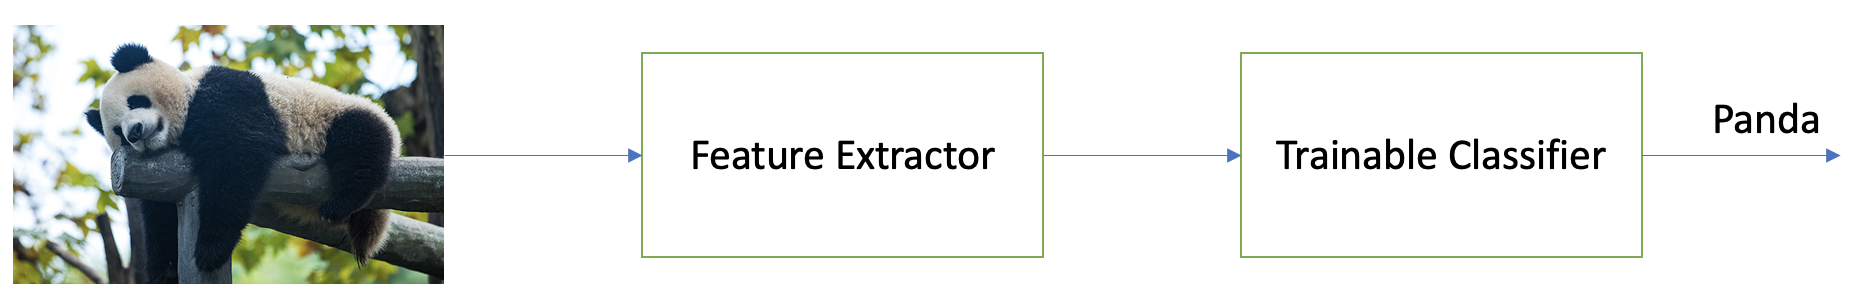
\includegraphics[width=0.9\textwidth]{images/deepLearning/functionalView/traditionalML.png}
    \caption{Flow of traditional machine learning}
    \label{fig:traditionalMLflow}
\end{figure}
The feature extraction is treated as a step independent of the classification. There are many different methods for feature extraction, for example, SIFT (scale-invariant feature transform). 

Deep learning, however, requires only one step (i.e., end-to-end) to implement both feature extraction and classification, as shown in Figure~\ref{fig:deeplearningflow}. 
\begin{figure}[!htbp]
    \centering
    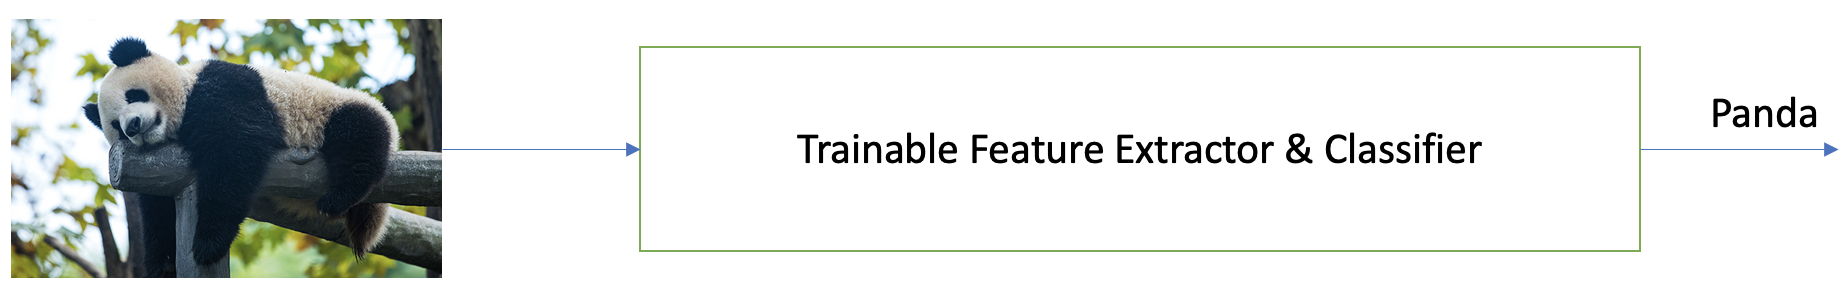
\includegraphics[width=0.9\textwidth]{images/deepLearning/functionalView/deeplearningflow.png}
    \caption{Flow of deep learning}
    \label{fig:deeplearningflow}
\end{figure}
Both the feature extractor and the classifier are trained at the same time. 

Feature extraction is closely related to dimensionality reduction, i.e., to separate data as much as possible. Most data distributions and tasks are non-linear, so a linear assumption is often convenient, but not necessarily truthful. Therefore, to get non-linear machines without too much effort, we may have to consider non-linear features. 

There are many ways to get non-linear features, including e.g., 
\begin{itemize}
    \item application of non-linear kernels, e.g., polynomial, RBF, etc.
    \item explicit design of features, e.g., SIFT, HOG, etc. 
\end{itemize}

The quality of features is usually evaluated against  the following few criteria: 
\begin{itemize}
    \item invariance
    \item repeatabilty 
    \item discriminativeness  
    \item robustness 
\end{itemize}
It is useful to note that these criteria may be conflicting. Hence, there needs to be a trade-off between criteria. 

\subsection*{Data manifold}

Actually, most natural, high-dimensional data (e.g. faces) lie on lower dimensional manifolds. For example, Figure~\ref{fig:swissRoll} is the so-called ``swiss roll'', where the data points are 3-dimensional, but they all lie on a 2-dimensional manifold. That is, the actual dimensionality of the manifold is 2, while the dimensionality of the input space is 3. 


\begin{figure}[!htbp]
    \centering
    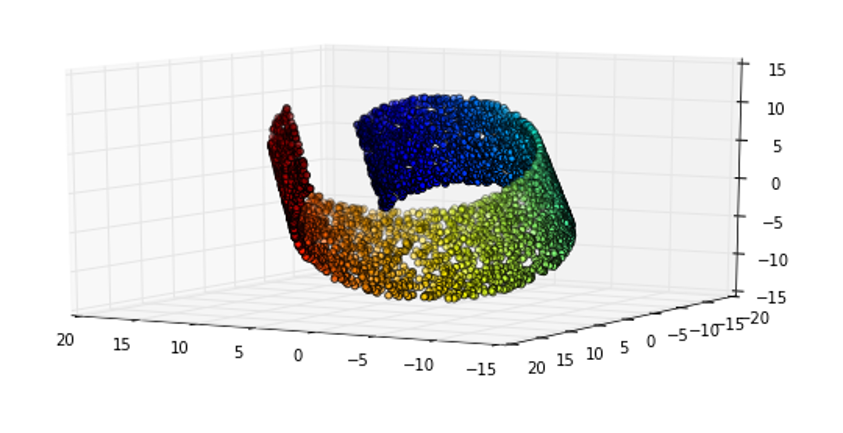
\includegraphics[width=0.7\textwidth]{images/deepLearning/functionalView/swissRoll.png}
    \caption{Data manifold -- ``swiss role'' example}
    \label{fig:swissRoll}
\end{figure}

Therefore, although the data points may consist of thousands of features, they can be described as a function of only a few underlying parameters. That is, the data points are actually sampled from a low-dimensional manifold that is embedded in a high-dimensional space. 

\subsection*{Difficulties of simply using dimensionality reduction or kernel}


The above observation suggests that our goal should be on discovering lower dimensional manifolds. We remark that, these manifolds are most probably highly non-linear. 

The success of this requires two hypotheses: 

\begin{itemize}
    \item If we can compute the coordinates of the input (e.g., a face image) to this non-linear manifold then the data become separable. This hypothesis suggests the existence of \emph{functional mapping}. For the ``swiss role'' example, there should be a (non-linear) function mapping from 3d space to 2d space, on which the data can be linearly separable.
    \item Semantically similar things lie closer than semantically dissimilar things. This implies the existence of applicable dimensional reduction methods. 
\end{itemize}







While raw data live in huge dimensionality, semantically meaningful raw data prefer lower dimensional manifolds, which still live in the same huge dimensionality. 
Can we discover this manifold to embed our data on? 


\subsection*{End-to-end learning of feature hierarchies}

The above discussions basically suggest that, it is an almost impossible task to manually craft features and also nontrivial to design algorithms (dimensionality reduction, functional mapping, etc) to compute features. This is in stark contrast with deep learning. Actually, one of the key advantages of convolutional neural networks is their ability to learn (or extract) features automatically.  

In a CNN, there are a pipeline of successive layers, such that each layer’s output is the input for the next layer. 
Layers produce features of higher and higher abstractions, such that the shadow layers extract low-level features (e.g. edges or corners), middle layers extract mid-level features (e.g. circles, squares, textures), and deep layers capture high level, class-specific features (e.g. face detector). See Figure~\ref{fig:featureVisualisation}. 

\begin{figure}[!htbp]
    \centering
    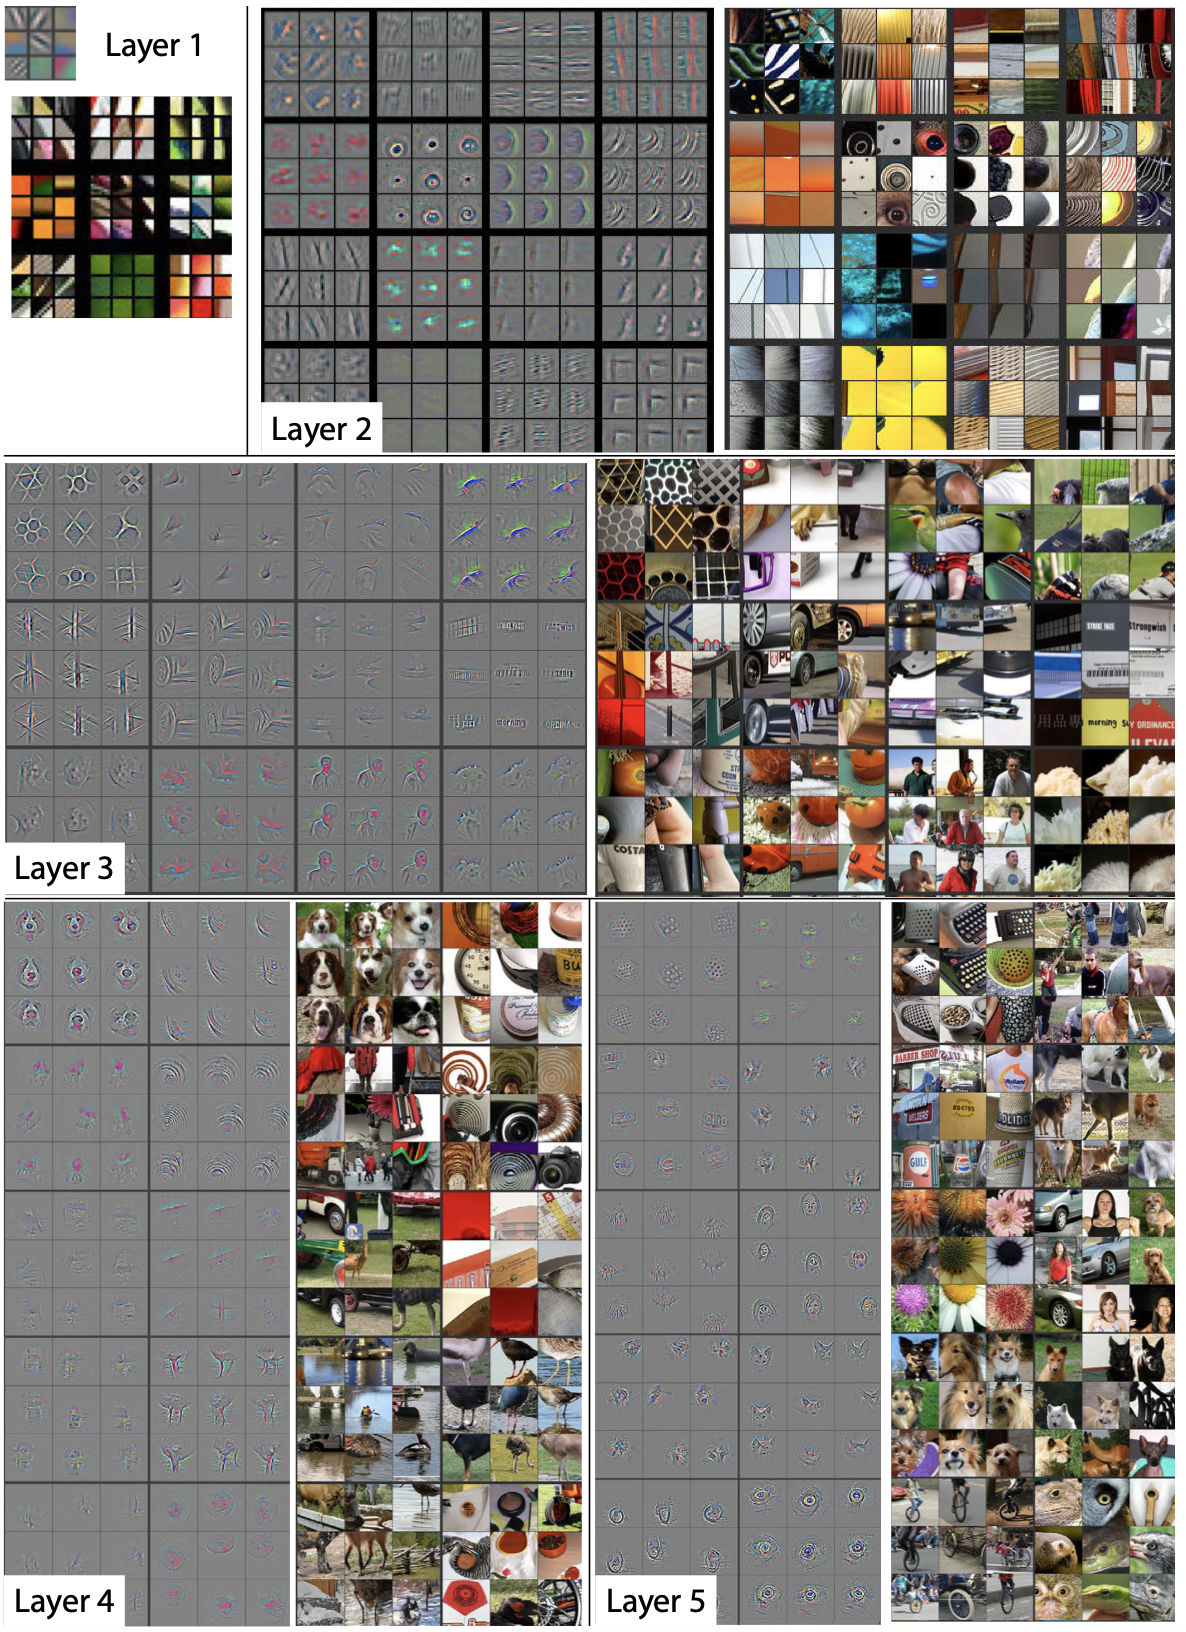
\includegraphics[width=\textwidth]{images/deepLearning/functionalView/featureVisualisation.png}
    \caption{Visualisation of features in hidden layers  \cite{DBLP:journals/corr/ZeilerF13}}
    \label{fig:featureVisualisation}
\end{figure}

We remark that, for CNNs, it has been shown that, preferably, training data should be as raw as possible. That is, no additional feature extraction phase  is needed. 



\subsection*{Why learn the features?}

Manually designed features 
often take a lot of time to come up with and implement, a lot of time to validate, and are incomplete, as one cannot know if they are optimal for the task. 
%
On the other hand, learned features 
are easy to adapt,  
very compact and specific to the task at hand. 
Given a basic architecture in mind, it is relatively easy and fast to optimize, i.e., 
time spent on designing features is now spent on designing architectures. 

\newpage
\subsection{Practice}

The following is a code to train a neural network with fully-connected layers. 

\subsection*{Train a fully connected model}

First of all, we install two packages torch and torchvision.

\begin{cmds}
pip3 install torch
pip3 install torchvision
\end{cmds}

Then, we set up hyper-parameters (e.g., batchsize, epoch, learning rate), device (e.g., CPU or GPU), and load training dataset (MNIST). 

\begin{lstlisting}[language=Python]
import torch
import torch.nn as nn
import torch.nn.functional as F
import torch.optim as optim
from torchvision import datasets, transforms
import argparse
import time

# Setup hyper-parameter
parser = argparse.ArgumentParser(description='PyTorch MNIST Training')
parser.add_argument('--batch-size', type=int, default=128, metavar='N',
                    help='input batch size for training (default: 128)')
parser.add_argument('--test-batch-size', type=int, default=128, metavar='N',
                    help='input batch size for testing (default: 128)')
parser.add_argument('--epochs', type=int, default=10, metavar='N',
                    help='number of epochs to train')
parser.add_argument('--lr', type=float, default=0.01, metavar='LR',
                    help='learning rate')
parser.add_argument('--no-cuda', action='store_true', default=False,
                    help='disables CUDA training')
parser.add_argument('--seed', type=int, default=1, metavar='S',
                    help='random seed (default: 1)')

args = parser.parse_args(args=[]) 

# Judge cuda is available or not
use_cuda = not args.no_cuda and torch.cuda.is_available()
#device = torch.device("cuda" if use_cuda else "cpu")
device = torch.device("cpu")

torch.manual_seed(args.seed)
kwargs = {'num_workers': 1, 'pin_memory': True} if use_cuda else {}

# Setup data loader
transform=transforms.Compose([
        transforms.ToTensor(),
        transforms.Normalize((0.1307,), (0.3081,))
        ])
trainset = datasets.MNIST('../data', train=True, download=True,
                   transform=transform)
testset = datasets.MNIST('../data', train=False,
                   transform=transform)
train_loader = torch.utils.data.DataLoader(trainset,batch_size=args.batch_size, shuffle=True,**kwargs)
test_loader = torch.utils.data.DataLoader(testset,batch_size=args.test_batch_size, shuffle=False, **kwargs)
\end{lstlisting}

We can define a fully connected network as follows, with the structure 784-128-64-32-10,

\begin{lstlisting}[language=Python]
# Define fully connected network
class Net(nn.Module):
    def __init__(self):
        super(Net, self).__init__()
        self.fc1 = nn.Linear(28*28, 128)
        self.fc2 = nn.Linear(128, 64)
        self.fc3 = nn.Linear(64, 32)
        self.fc4 = nn.Linear(32, 10)

    def forward(self, x):
        x = self.fc1(x)
        x = F.relu(x)
        x = self.fc2(x)
        x = F.relu(x)
        x = self.fc3(x)
        x = F.relu(x)
        x = self.fc4(x)
        output = F.log_softmax(x, dim=1)
        return output
\end{lstlisting}

Then, we define the training function, which computes loss and updates parameters for each minibatch. 

\begin{lstlisting}[language=Python]
# Training function
def train(args, model, device, train_loader, optimizer, epoch):
    model.train()
    for batch_idx, (data, target) in enumerate(train_loader):
        data, target = data.to(device), target.to(device)
        data = data.view(data.size(0),28*28)
        
        # Clear gradients
        optimizer.zero_grad()
        
        # Compute loss
        loss = F.cross_entropy(model(data), target)
        
        # Get gradients and update
        loss.backward()
        optimizer.step()
\end{lstlisting}

We also can define a predict function, which outputs training loss and test loss for each epoch. 

\begin{lstlisting}[language=Python]
# Predict function
def eval_test(model, device, test_loader):
    model.eval()
    test_loss = 0
    correct = 0
    with torch.no_grad():
        for data, target in test_loader:
            data, target = data.to(device), target.to(device)
            data = data.view(data.size(0),28*28)
            output = model(data)
            test_loss += F.cross_entropy(output, target, size_average=False).item()
            pred = output.max(1, keepdim=True)[1]
            correct += pred.eq(target.view_as(pred)).sum().item()
    test_loss /= len(test_loader.dataset)
    test_accuracy = correct / len(test_loader.dataset)
    return test_loss, test_accuracy
\end{lstlisting}

Finally, we define the main function and call the training function for each epoch.

\begin{lstlisting}[language=Python]
# Main function, train the dataset and print training loss, test loss
def main():
    model = Net().to(device)
    optimizer = optim.SGD(model.parameters(), lr=args.lr)
    for epoch in range(1, args.epochs + 1):
        start_time = time.time()
        
        # Training
        train(args, model, device, train_loader, optimizer, epoch)
        
        # Get trnloss and testloss
        trnloss, trnacc = eval_test(model, device, train_loader)
        tstloss, tstacc = eval_test(model, device, test_loader)
        
        # Print trnloss and testloss
        print('Epoch '+str(epoch)+': '+str(int(time.time()-start_time))+'s', end=', ')
        print('trn_loss: {:.4f}, trn_acc: {:.2f}%'.format(trnloss, 100. * trnacc), end=', ')
        print('test_loss: {:.4f}, test_acc: {:.2f}%'.format(tstloss, 100. * tstacc))

if __name__ == '__main__':
    main()
\end{lstlisting}




%\newpage
\section{Forward and Backward Computation}

In Section~\ref{sec:perceptron}, we have explained that a multi-layer perceptron has more expressive power than a single-layer perceptron. In particular, it is able to find a two-layer perceptron to solve the XOR problem, while it is not possible for a single-layer perceptron. However, we did not explain in  Section~\ref{sec:perceptron} how to compute the weights for the two-layer perceptron for XOR. Moreover, we note that, the perceptron learning algorithm cannot be used for learning multi-layer perceptron. Actually, the learning algorithm for multi-layer perceptron, called backpropagation (BP), is one of the key milestones for the development of deep learning. 

The BP algorithm computes the gradient of the loss function with respect to each weight by the chain rule. Instead of computing one gradient for each weight, it is able to compute
the gradient for one layer at a time, and more importantly, it is able to iterate backwards from the last layer to avoid redundant calculations of intermediate terms in the chain rule. This makes it efficient enough to train large scale neural networks. 

The BP algorithm is the foundation of deep learning, and in this section, we use a running example to explain its computation. 

\subsection*{Running Example}

In this example, we have three layers, one input layer, one hidden layer, and one output layer. Each layer has two neurons. The connections between neurons are given in the left diagram of Figure~\ref{fig:network}. 

\begin{figure}[!htbp]
    \centering
    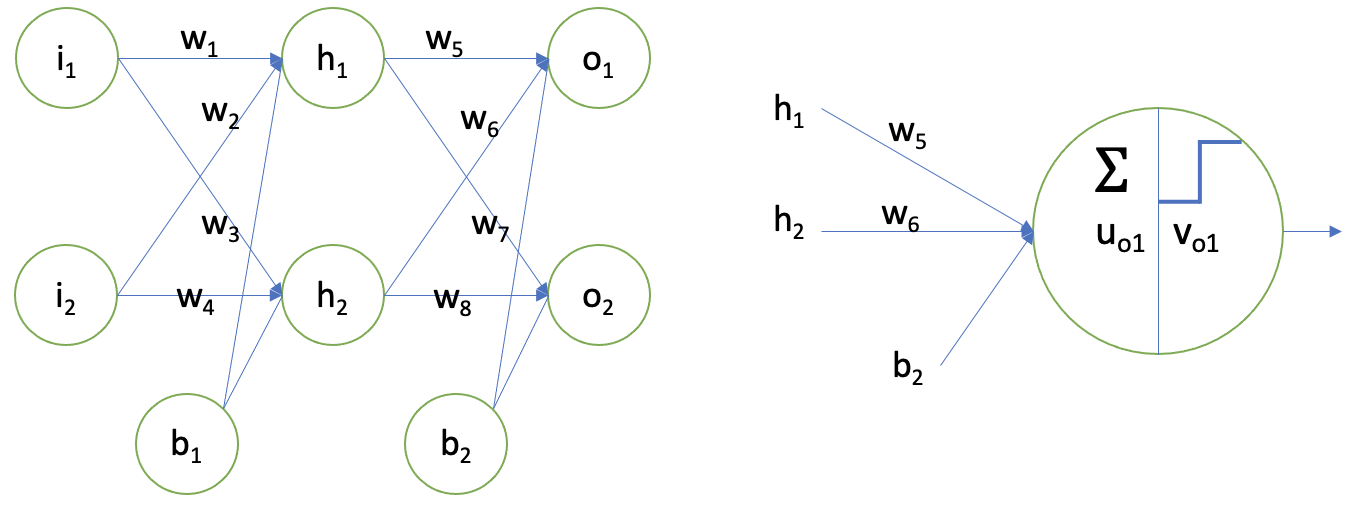
\includegraphics[width=0.8\textwidth]{images/deepLearning/propagation/network.png}
    \caption{A simple neural network with a hidden layer (Left) and the illustration of a neuron with activation function (Right)}
    \label{fig:network}
\end{figure}

The diagram on the right is an illustration of a neuron with an activation function. Each neuron has two values $u$ and $v$, representing its values before and after the application of the activation function, respectively. 

The learning is a dynamic process with weights continuously updated until convergence. Now,  we assume that, at some point, the current weights are 
\begin{equation}
\begin{blockarray}{cc}
\begin{block}{(cc)}
   w_1 & w_2 \\
   w_3 & w_4 \\
\end{block}
\end{blockarray} = 
\begin{blockarray}{cc}
\begin{block}{(cc)}
   0.15 & 0.20 \\
   0.25 & 0.30 \\
\end{block}
\end{blockarray}\text{~~ , ~~}
\begin{blockarray}{cc}
\begin{block}{(cc)}
   w_5 & w_6 \\
   w_7 & w_8 \\
\end{block}
\end{blockarray} = 
\begin{blockarray}{cc}
\begin{block}{(cc)}
   0.40 & 0.45 \\
   0.50 & 0.55 \\
\end{block}
\end{blockarray}
\text{~~ , ~~}
\begin{blockarray}{c}
\begin{block}{(c)}
   b_1 \\
   b_2 \\
\end{block}
\end{blockarray} = 
\begin{blockarray}{c}
\begin{block}{(c)}
   0.35 \\
   0.60 \\
\end{block}
\end{blockarray}
\end{equation}

Note that, every row in a weight matrix stores the input weights for a neuron, for example, the row $(0.15~~0.20)$ is associated with the neuron $h_1$. Also, each entry in a bias vector represents a bias for a layer. 


\subsection{Forward Computation}

The first step of each iteration of the BP algorithm is to compute the loss by making a forward computation. 
%
Assume that we have an input $\textbf{x}=(0.05,0.10)^T$ for the network in Figure~\ref{fig:network}, we can have  

\begin{equation}
\begin{blockarray}{c}
\begin{block}{(c)}
   u_{h_1} \\
   u_{h_2} \\
\end{block}
\end{blockarray} = 
\begin{blockarray}{cc}
\begin{block}{(cc)}
   0.15 & 0.20 \\
   0.25 & 0.30 \\
\end{block}
\end{blockarray} \times 
\begin{blockarray}{c}
\begin{block}{(c)}
   0.05 \\
   0.10 \\
\end{block}
\end{blockarray} +  
\begin{blockarray}{c}
\begin{block}{(c)}
   0.35 \\
   0.35 \\
\end{block}
\end{blockarray} =
\begin{blockarray}{c}
\begin{block}{(c)}
   0.3775 \\
   0.6425 \\
\end{block}
\end{blockarray}
\end{equation}
Assume that the network uses the Sigmoid function $\sigma$ as the activation function, we have 
\begin{equation}
    \begin{blockarray}{c}
\begin{block}{(c)}
   v_{h_1} \\
   v_{h_2} \\
\end{block}
\end{blockarray} = \sigma(
    \begin{blockarray}{c}
\begin{block}{(c)}
   0.3775 \\
   0.3925 \\
\end{block}
\end{blockarray}) \approx 
\begin{blockarray}{c}
\begin{block}{(c)}
   0.5927 \\
   0.5969 \\
\end{block}
\end{blockarray}
\end{equation}
as the output of the hidden layer. 
%
On the output layer, we have 
\begin{equation}
\begin{blockarray}{c}
\begin{block}{(c)}
   u_{o_1} \\
   u_{o_2} \\
\end{block}
\end{blockarray} = 
\begin{blockarray}{cc}
\begin{block}{(cc)}
   0.40 & 0.45 \\
   0.50 & 0.55 \\
\end{block}
\end{blockarray} \times 
\begin{blockarray}{c}
\begin{block}{(c)}
   0.5927 \\
   0.5969 \\
\end{block}
\end{blockarray} +  
\begin{blockarray}{c}
\begin{block}{(c)}
   0.60 \\
   0.60 \\
\end{block}
\end{blockarray} =
\begin{blockarray}{c}
\begin{block}{(c)}
   1.1057 \\
   1.2247 \\
\end{block}
\end{blockarray}
\end{equation}
Consider the Sigmoid function, we have 
\begin{equation}
\begin{blockarray}{c}
\begin{block}{(c)}
   v_{o_1} \\
   v_{o_2} \\
\end{block}
\end{blockarray} =
    \sigma(
    \begin{blockarray}{c}
\begin{block}{(c)}
   1.1057 \\
   1.2247 \\
\end{block}
\end{blockarray}) \approx 
\begin{blockarray}{c}
\begin{block}{(c)}
   0.7513 \\
   0.7729 \\
\end{block}
\end{blockarray}
\end{equation}
as the output of the output layer. That is, $\hat y=(0.7513,0.7729)$. 
%
Now, assuming that the label of $\textbf{x}$ is $y=(0.01,0.99)^T$ and we are using the mean square error, we can compute the loss for 
\begin{equation}
    L(\textbf{x},y) = \frac{1}{2}(0.7513-0.01)^2 + \frac{1}{2}(0.7729-0.99)^2 \approx 0.2748 +0.0236= 0.2984
\end{equation}
where we let $L_{o1}(\textbf{x},y)=\frac{1}{2}(0.7513-0.01)^2$ and $L_{o2}(\textbf{x},y)=\frac{1}{2}(0.7729-0.99)^2$, representing the loss of individual neurons $o_1$ and $o_2$, respectively. 

\subsection{Backward Computation}


Once we have the loss ${L}(\textbf{x},y)$, we can start back-propagation by applying the chain rule. 
%

\subsection*{Weights of output neurons}

First of all, for the weights of output neuron, such as $w_5$, we can compute as follows: 

\begin{equation}\label{equ:backpropoutput}
    \frac{{\partial L}}{{\partial w_5}} = \frac{{\partial L_{o_1}}}{{\partial v_{o_1}}}*\frac{{\partial v_{o_1}}}{{\partial u_{o_1}}}*\frac{{\partial u_{o_1}}}{{\partial w_5}}
\end{equation}
Figure~\ref{fig:backoutput} presents an  illustrative diagram for the Equation (\ref{equ:backpropoutput}). 
\begin{figure}[!htbp]
    \centering
    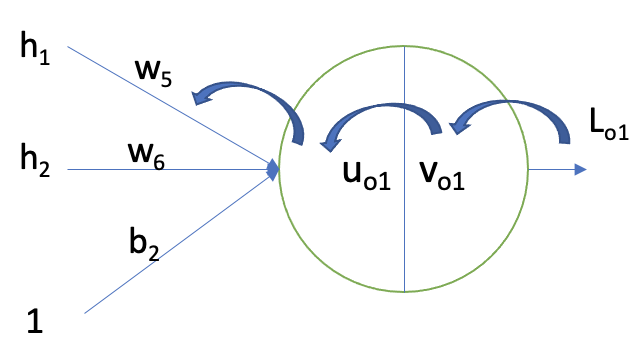
\includegraphics[width=0.4\textwidth]{images/deepLearning/propagation/back.png}
    \caption{Backward propagation on the output neuron}
    \label{fig:backoutput}
\end{figure}
Actually, the backpropagation goes from the loss $L_{o_1}$ to the value $v_{o_1}$, $u_{o_1}$, until the weight $w_5$. 

Concretely, for the running example, we have 
\begin{equation}
     \displaystyle\frac{{\partial L_{o_1}}}{{\partial v_{o_1}}}=\frac{{\partial }}{{\partial v_{o_1}}}(\frac{1}{2}(y^{(1)}-v_{o_1})^2) = -(y^{(1)}-v_{o_1}) = 0.7513-0.01 = 0.74  \\
\end{equation}
where $y^{(1)}$ is the first component of $y$, and 
\begin{equation}
\frac{{\partial v_{o_1}}}{{\partial u_{o_1}}} =  \frac{{\partial \sigma(u_{o_1})}}{{\partial u_{o_1}}} = \sigma(u_{o_1})(1-\sigma(u_{o_1})) = v_{o_1}(1-v_{o_1}) \approx 0.7513\times 0.2487\approx 0.1868
\end{equation}
and 
\begin{equation}
    \frac{{\partial u_{o_1}}}{{\partial w_5}}=\frac{{\partial }}{{\partial w_5}}(w_5v_{h_1}+w_6v_{h_2}+b_2)= v_{h_1} \approx 0.5927
\end{equation}
Therefore, we have 
\begin{equation}
    \frac{{\partial L}}{{\partial w_5}} = \frac{{\partial L_{o_1}}}{{\partial v_{o_1}}}*\frac{{\partial v_{o_1}}}{{\partial u_{o_1}}}*\frac{{\partial u_{o_1}}}{{\partial w_5}}\approx 0.74 \times 0.1868 \times  0.5927 = 0.0819
\end{equation}

\subsection*{Weights of hidden neurons}

Now, the weight of hidden layer can be done recursively by applying the chain rules, e.g., 
\begin{equation}\label{equ:backprophidden}
\begin{array}{rcl}
   \displaystyle  \frac{{\partial L}}{{\partial w_1}} 
   &  = & \displaystyle \frac{{\partial L}}{{\partial v_{h_1}}}*\frac{{\partial v_{h_1}}}{{\partial u_{h_1}}}*\frac{{\partial u_{h_1}}}{{\partial w_1}} \\ 
    & = & \displaystyle (\frac{{\partial L_{o_1}}}{{\partial v_{h_1}}}+\frac{{\partial L_{o_2}}}{{\partial v_{h_1}}})*\frac{{\partial v_{h_1}}}{{\partial u_{h_1}}}*\frac{{\partial u_{h_1}}}{{\partial w_1}} \\
    & = & \displaystyle (\frac{{\partial L_{o_1}}}{{\partial u_{o_1}}}\frac{{\partial u_{o_1}}}{{\partial u_{h_1}}}+\frac{{\partial L_{o_2}}}{{\partial u_{o_2}}}\frac{{\partial u_{o_2}}}{{\partial u_{h_1}}})*\frac{{\partial v_{h_1}}}{{\partial u_{h_1}}}*\frac{{\partial u_{h_1}}}{{\partial w_1}}\\
    & = & \displaystyle (\frac{{\partial L_{o_1}}}{{\partial u_{o_1}}}w_5+\frac{{\partial L_{o_2}}}{{\partial u_{o_2}}}w_7)*\frac{{\partial v_{h_1}}}{{\partial u_{h_1}}}*\frac{{\partial u_{h_1}}}{{\partial w_1}}
\end{array}
\end{equation}
Note that, all the components of Equation (\ref{equ:backprophidden}) can now be computed as the method we used for the output layer. Figure~\ref{fig:backhidden} presents an illustration of backward propagation as in Equation (\ref{equ:backprophidden}). 

\begin{figure}[!htbp]
    \centering
    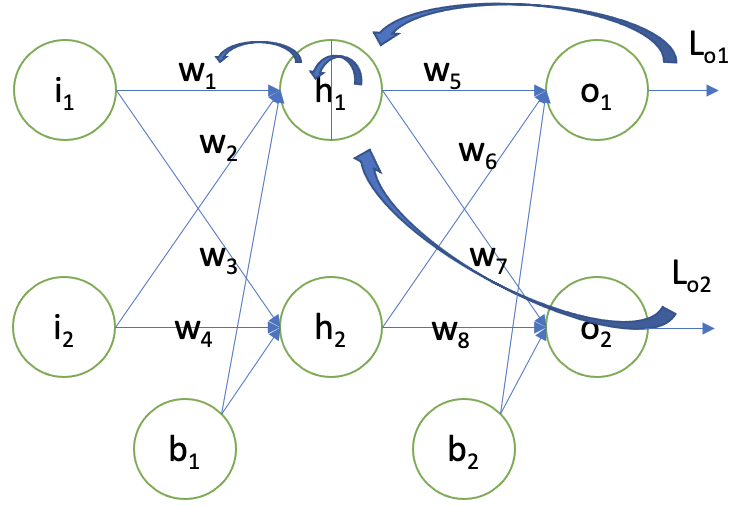
\includegraphics[width=0.45\textwidth]{images/deepLearning/propagation/back2.png}
    \caption{Backward propagation on the hidden neuron}
    \label{fig:backhidden}
\end{figure}

\subsection*{Weight update}

Finally, once we compute the gradients $\displaystyle  \frac{{\partial L}}{{\partial w_5}}$ or $\displaystyle  \frac{{\partial L}}{{\partial w_1}}$, we can update the weights $w_5$ or $w_1$ by applying the gradient descent algorithm. We remark that, while the above computation is conducted for individual weights, the BP algorithm can work on a layer basis to significantly improve the efficiency. 

\subsection{Regularisation as Constraints}

In general, regularisation is a set of methods to  prevent overfitting or help the optimization. Typically, this is done by having additional terms in the training optimisation objective. 

\subsection*{Overfitting}

Overfitting is a concept closely related to the generalisation error as introduced in Section~\ref{sec:generalisationerror}, which is the gap between empirical loss and expected loss. 
It has been observed that, the following two reasons may contribute as the key to the overfitting. 

\begin{itemize}
    \item dataset is too small
    \item hypothesis space is too large
\end{itemize}

To understand the second point, we note that, the larger the hypothesis space, the easier is for a learning algorithm to find a hypothesis that has small training error. However, finding a small training error does not warrant the found hypothesis can be of a small test error, and so this may lead to large test error (overfitting). This observation suggests that it might be beneficial to leave out useless hypotheses, which is what regularization is for. 

\subsection*{Regularization as hard constraint}

Assume that, for a dataset $D=(\textbf{X},\textbf{y})$ of $n$ training instances, we have the following optimising objective: 
\begin{equation}
\begin{array}{rl}
    \displaystyle\min_f & \displaystyle L(f,D) = \frac{1}{n} \sum_{i=1}^n L(f,\textbf{x}_i,y_i) \\
    \text{subject to } & f\in {\cal H}
\end{array}
\end{equation}
Considering that for a deep learning model, $f$ is parameterised over the weights $W$, we have 
\begin{equation}
\begin{array}{rl}
    \displaystyle\min_W & \displaystyle L(W,D) = \frac{1}{n} \sum_{i=1}^n L(W,\textbf{x}_i,y_i) \\
    \text{subject to } & W\in {\cal \real^{|W|}}
\end{array}
\end{equation}
where $|W|$ is the number of weights. 

The regularisation is to add further constraints. For example, if we ask for $L_2$ regularisation, we have 
\begin{equation}
\begin{array}{rl}
    \displaystyle\min_W & \displaystyle L(W,D) = \frac{1}{n} \sum_{i=1}^n L(W,\textbf{x}_i,y_i) \\
    \text{subject to } & W\in {\cal \real^{|W|}}\\
    & ||W||_2^2 \leq r^2
\end{array}
\end{equation}
for some pre-specified $r>0$. 

\subsection*{Regularization as soft constraint}

While the hard constraints limit the selection of hypothesis, it might not be easy to be integrated with the backpropagation algorithm, which does not consider the constraints directly. This can be done through a soft constraint, e.g., 

\begin{equation}
\begin{array}{rl}
    \displaystyle\min_W & \displaystyle L(W,D) = \frac{1}{n} \sum_{i=1}^n L(W,\textbf{x}_i,y_i) + \lambda ||W||_2^2 \\
\end{array}
\end{equation}
where $\lambda$ is a hyper-parameter to balance between the loss term and the constraint/penalty term. Alternatively, this can be done through Lagrangian multiplier method: 
\begin{equation}
\begin{array}{rl}
    \displaystyle\min_W & \displaystyle L(W,D) = \frac{1}{n} \sum_{i=1}^n L(W,\textbf{x}_i,y_i) + \lambda (||W||_2^2-r) \\
\end{array}
\end{equation}


\subsection{Practice}

The following code is to save the weights of a trained model and load the weights from a file. 

\begin{lstlisting}[language=Python]
# Save model
torch.save(model.state_dict(), 'model.pt')

# Load model
model.load_state_dict(torch.load('model.pt'))
\end{lstlisting}



%\newpage
\section{Convolutional Neural Networks}

This section introduces a specific class of neural networks that has been shown very effective in processing images. 
%
In 1998, Yann LeCun and his collaborators developed a neural network for handwritten digits called LeNet \cite{726791}. It is a feedforward network with several hidden layers, trained with the backpropagation algorithm. It is later formalised with the name  convolutional neural networks (CNNs). Since LeNet, there are many other variants of CNNs, such as AlexNet, VGG16, ResNet, GoogLeNet, and so on. These variants introduce new functional layers or training methods that help improve the performance of the CNNs in pattern recognition tasks. 


\begin{figure}[!htbp]
    \centering
    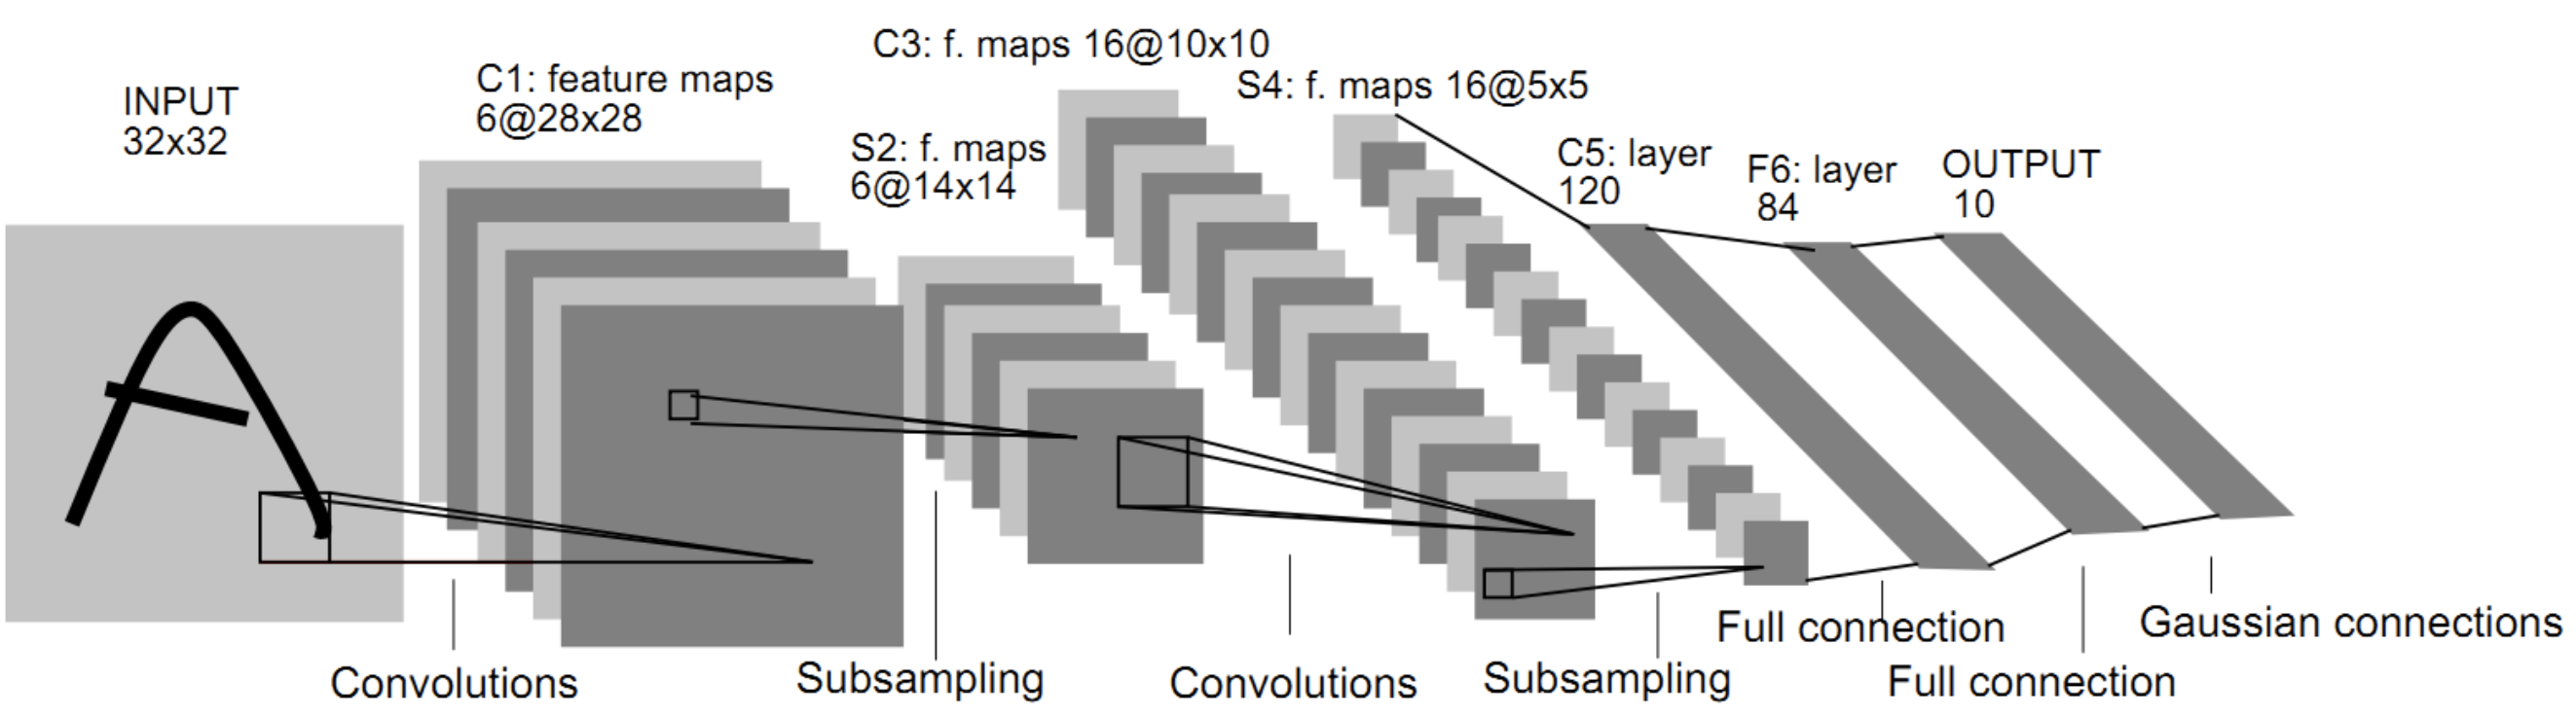
\includegraphics[width=\textwidth]{images/deepLearning/CNN/LeNet.png}
    \caption{Architecture of LeNet-5 \cite{726791}, a convolutional neural network for digits recognition. }
    \label{fig:LeNet}
\end{figure}


As shown in Figure~\ref{fig:LeNet}, LeNet has an input layer, 6 hidden layers, and an output layer. Among the 4 hidden layers, there are 2 convolutional layers, 2 subsampling (or pooling) layers, and 2 fully connected layers. 
%
Actually, common functional layers of a CNN can be e.g., fully-connected layers, convolutional layers, pooling layers, etc. It is very often that a functional layer is followed by an activation layer, such as ReLU layer, Sigmoid layer, Tanh layer, etc. After a sequence of functional and activation layers, we need a softmax layer to convert the output into a probability distribution. 

In the following, we first introduce functional layers, activation functions, and softmax layer that have been widely used in various CNNs, and then present a few common practices that have been used to either prepare data for training in or support the training. 



\subsection{Functional Layers}\label{sec:functionallayers}

As suggested earlier, each layer function $f_i$ is a mapping from a high-dimensional space $\real^{k_{i-1}}$ (that associates with Layer-$(i-1)$) to another $\real^{k_{i}}$ (that associates with Layer-$i$). That is, given $\textbf{v}_{i-1}\in \real^{k_{i}}$, we have $\textbf{v}_{i}=f_{i}(\textbf{v}_{i-1})\in \real^{k_{i}}$. 

Actually, in most CNN layers, the transformation $f_{i}$ is conducted in two steps. For the first step, it is transformed with a linear transformation, and in the second step, every neuron passes through an activation function. Formally, 
\begin{equation}
    \textbf{u}_{i}=\textbf{W}_{i}\textbf{v}_{i-1}+\textbf{b}_i \text{~~~~ and ~~~~} \textbf{v}_{i} = \sigma_i(\textbf{u}_{i})
\end{equation}
where $\sigma_i$ is an activation function. In the following, we introduce functional layers, followed by activation functions. 


\subsubsection{Fully-connected Layer}

In a fully connected layer, every neuron
receives inputs from all neurons of the previous layer, and the output of the neuron is the result of the linear combination of the inputs.  As shown in Figure~\ref{fig:fully-connected}, Layer 2 is a fully-connected layer. The neuron $n_{21}$ receives inputs from all neurons $n_{11},...,n_{16}$ in Layer 1, and weighted them with the learnable weights $\textbf{W}_{21}=(w_{21,11},...,w_{21,16})$. Therefore, its value 
\begin{equation}
    u_{21} = \textbf{W}_{21}\times \textbf{v}_1 + b_2 = w_{21,11}v_{11} + ... + w_{21,16}v_{16} + b_2
\end{equation}
where $b_2$ is the bias of layer 2. Similar for the neuron $n_{22}$. 

Note that, in the above, we use symbol $u$, instead of $v$, to denote the value of the neuron, because the output of this neuron normally needs to pass through an activation function, i.e., 
\begin{equation}
    v_{21} = \alpha(u_{21}) 
\end{equation}
We will introduce activation functions $\alpha$ later. 

\begin{figure}[!htbp]
    \centering
    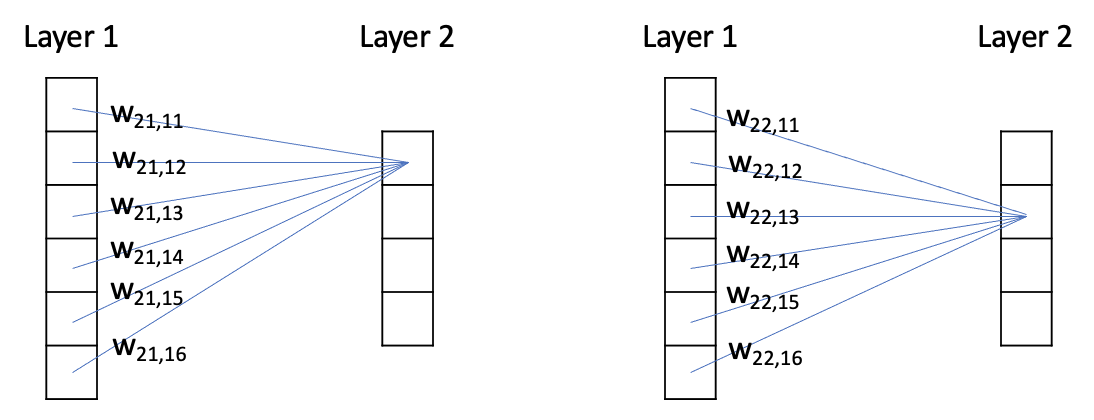
\includegraphics[width=0.7\textwidth]{images/deepLearning/CNN/fully-connected.png}
    \caption{Illustration of fully-connected layer}
    \label{fig:fully-connected}
\end{figure}

In a CNN, fully connected layers often appear in the last few layers, after the convolutional layers. The main functionality of those fully-connected layers is to implement classification over those features extracted by the convolutional layers.  
 

\subsubsection{Convolutional Layer}

Given an $n\times n$ matrix $\textbf{x}$ and an $m\times m$ filter $\textbf{f}$, we can compute the resulting matrix $\textbf{z}$ by repeatedly (1) overlapping the filter over the matrix, as illustrated in Figure~\ref{fig:convolutinallayer} with the red dashed lines,  and (2) computing an element $z_{i,j}$ with element-wise multiplication, as illustrated in Figure~\ref{fig:convolutinallayer} with the blue dashed lines.

The overlapping usually starts from the element (1,1) of the matrix $\textbf{x}$. Therefore, the (1,1) element in the resulting matrix $\textbf{z}$ is computed as follows with the element-wise multiplication: 
\begin{equation}
    z_{1,1} = \sum_{k=0}^{m-1}\sum_{l=0}^{m-1} x_{1+k,1+l}\times f_{1+k,1+l}
\end{equation}

Afterwards, it depends on a parameter $stride$ to determine the next element on $\textbf{x}$. For example, if $stride=1$, then one of the next elements, along the horizontal direction, is $(1,1+stride)= (1,2)$ such that  
\begin{equation}
    z_{1,2} = \sum_{k=0}^{m-1}\sum_{l=0}^{m-1} x_{1+k,1+l+stride}\times f_{1+k,1+l}= \sum_{k=0}^{m-1}\sum_{l=0}^{m-1} x_{1+k,1+l+1}\times f_{1+k,1+l}
\end{equation}
The other next element, along the vertical direction, is $(1+stride,1)= (2,1)$ such that  
\begin{equation}
    z_{2,1} = \sum_{k=0}^{m-1}\sum_{l=0}^{m-1} x_{1+k+stride,1+l}\times f_{1+k,1+l}= \sum_{k=0}^{m-1}\sum_{l=0}^{m-1} x_{1+k+1,1+l}\times f_{1+k,1+l}
\end{equation}
Figure~\ref{fig:convolutinallayer} presents the case where we move horizontally with $stride=1$. 

If $stride=2$, the next horizontal  element on $\textbf{x}$ will be $(1,1+stride)=(1,3)$ and we are computing the $(1,2)$ element for the resulting matrix $\textbf{z}$, i.e., 
\begin{equation}
    z_{1,2} = \sum_{k=0}^{m-1}\sum_{l=0}^{m-1} x_{1+k,1+l+stride}\times f_{1+k,1+l}= \sum_{k=0}^{m-1}\sum_{l=0}^{m-1} x_{1+k,1+l+2}\times f_{1+k,1+l}
\end{equation}
Similarly, the next vertical  element $(2,1)$ is computed as follows: 
\begin{equation}
    z_{2,1} = \sum_{k=0}^{m-1}\sum_{l=0}^{m-1} x_{1+k+stride,1+l}\times f_{1+k,1+l}= \sum_{k=0}^{m-1}\sum_{l=0}^{m-1} x_{1+k+2,1+l}\times f_{1+k,1+l}
\end{equation}
Note that, no matter what the $stride$ is, the incremental to the element on $\textbf{z}$ is always 1, to make sure that we are constructing $\textbf{z}$ one element by one element. 


\begin{figure}[!htbp]
    \centering
    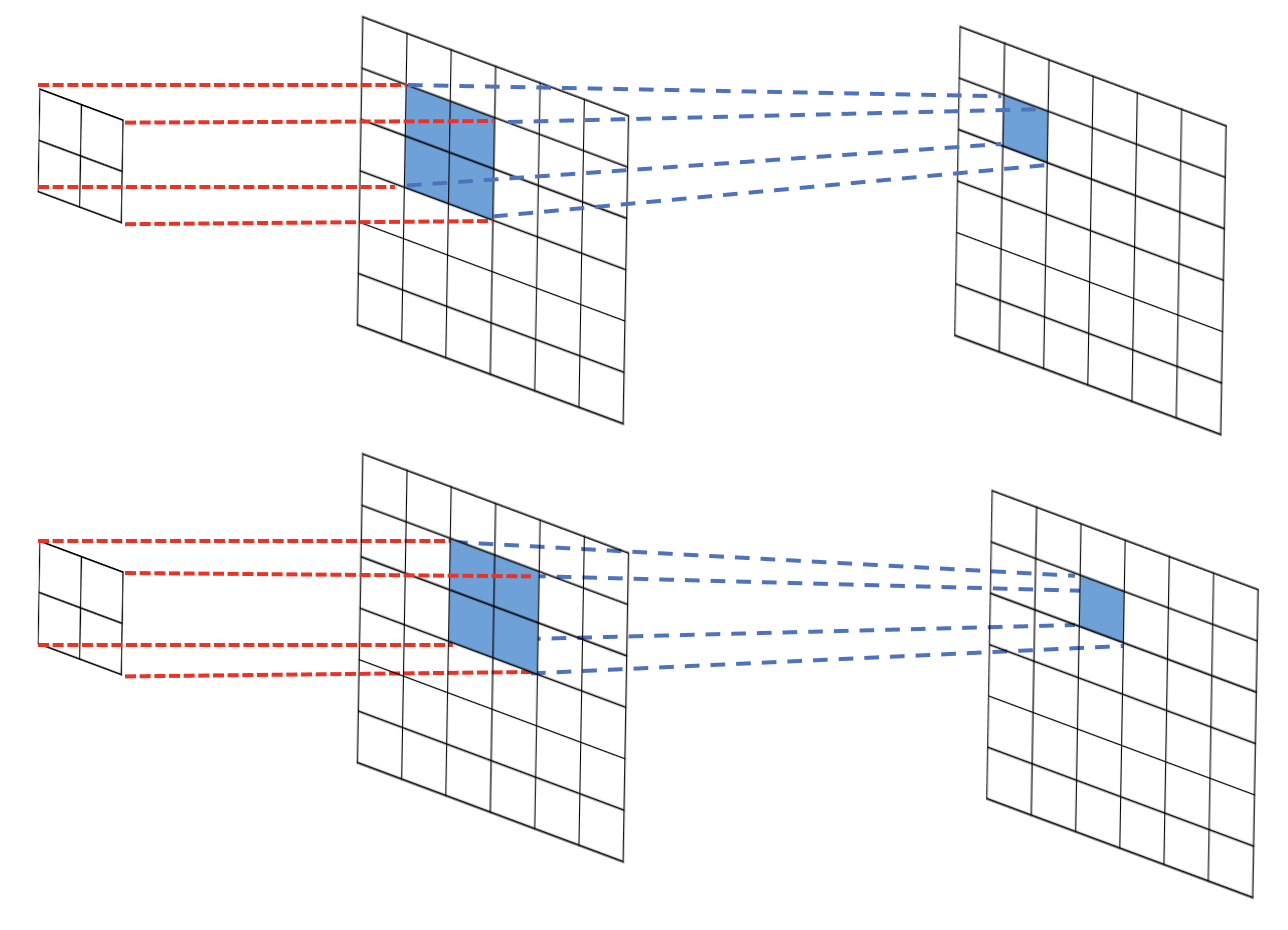
\includegraphics[width=0.9\textwidth]{images/deepLearning/CNN/convolutional.png}
    \caption{Illustration of convolutional layer}
    \label{fig:convolutinallayer}
\end{figure}

We can see that, $\textbf{z}$ is a $t\times t$ matrix such that 
\begin{equation}
    t = \frac{n-m}{stride}+1
\end{equation}
For example, if $n=4$ and $m=2$, then $t=3$ when $stride=1$ and $t=2$ when $stride=2$. 

\subsubsection{Zero-Padding}

As we can see from the previous discussion on the convolutional layer, the shapes of the matrices $\textbf{x}$ and $\textbf{z}$ are not the same. It is possible that we might be interested in maintaining the shape of the matrix along a sequence of convolutional operations. In this case, it is useful to consider a pre-processing on $\textbf{x}$ before the convolutional filter is applied. 
%
Zero-padding, a typical pre-processing operation, is to use 0 to pad the input with 0-cells, as shown in Figure~\ref{fig:zeropadding}. 

\begin{figure}
    \centering
    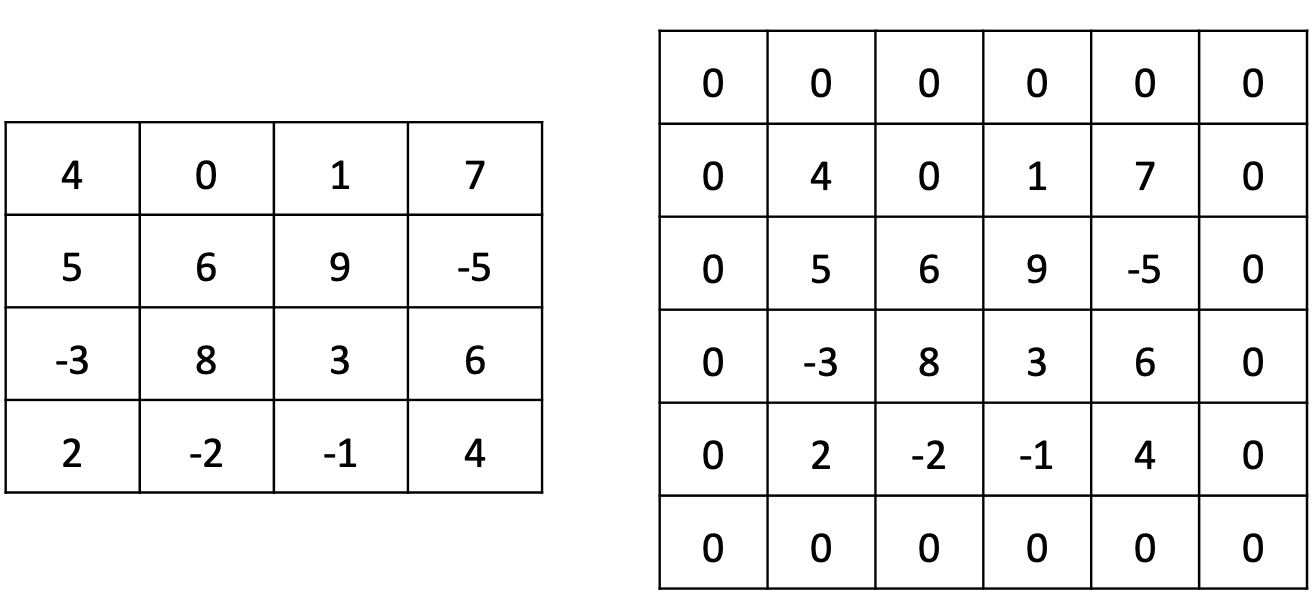
\includegraphics[width=0.6\textwidth]{images/deepLearning/CNN/padding.png}
    \caption{Zero-padding: pad the input with 0-cells around it. }
    \label{fig:zeropadding}
\end{figure}

We can see that,  if we pad $\textbf{x}$ with a border of $u$ zero valued pixels, $\textbf{z}$ is a $t\times t$ matrix such that 
\begin{equation}
    t = \frac{n-m+2*u}{stride}+1
\end{equation}
In Figure~\ref{fig:zeropadding}, $u=1$. Therefore, if $n=4$ and $m=2$ and $u=1$, then $t=5$ when $stride=1$ and $t=3$ when $stride=2$. 

\subsubsection{Pooling Layer}

A pooling layer is to reduce the information in a matrix by collapsing elements with operations. The pooling layer is frequently used in convolutional neural networks with the purpose of progressively reducing the spatial size of the representation to reduce the number of features and the computational complexity of the network. Assume that, as shown in Figure~\ref{fig:maxpooling}, we have a $4\times 4$ matrix. An application of a $2\times 2$ max-pooling filter, under the condition that $stride = 2$, will get a $2\times 2$ matrix by collapsing every $2\times 2$ block with the $\max$ operation. 

 
 
 \begin{figure}
    \centering
    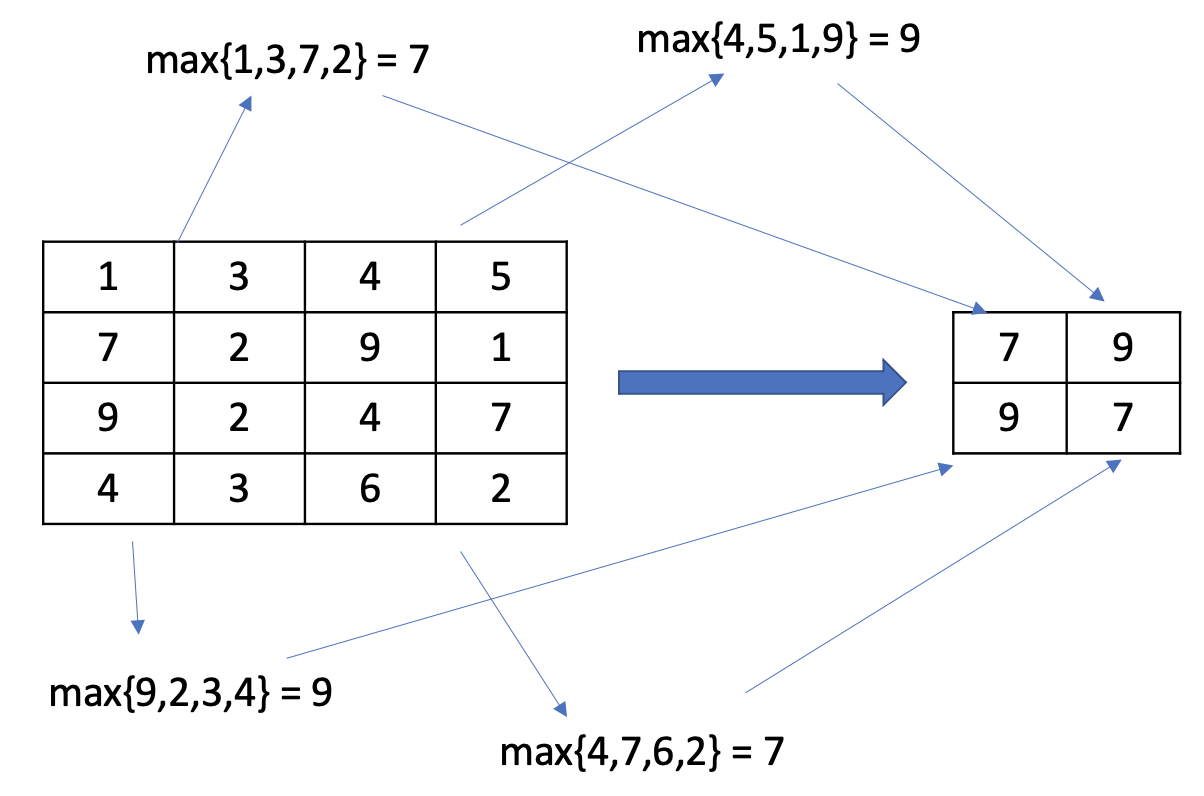
\includegraphics[width=0.6\textwidth]{images/deepLearning/CNN/maxpooling.png}
    \caption{Max-pooling. An application of $2\times 2$ filter, $stride=2$, on a $4\times 4$ matrix.}
    \label{fig:maxpooling}
\end{figure}

In addition to max-pooling, there are other pooling layers, such as the average-pooling layer, which replaces the $\max$ operation with the average operation. 


\subsection{Activation Functions}

As mentioned earlier, for most functional layers, they are followed by an activation layer where 

\subsection*{ReLU}

\begin{equation}
    ReLU(x) = max(0,x)
\end{equation}

\subsection*{Sigmoid}

\begin{equation}
    \sigma(x) = \frac{1}{1+e^{-x}}
\end{equation}
such that $\sigma'(x)=\sigma(x)(1-\sigma(x))$. 

\subsection*{Softmax}

\begin{equation}
    \delta(\textbf{v}) = (\frac{e^{v_1}}{\sum_{i=1}^{|\textbf{v}|}e^{v_i}},...,\frac{e^{v_{|\textbf{v}|}}}{\sum_{i=1}^{|\textbf{v}|}e^{v_i}}) 
\end{equation}

\subsection{Data Preprocessing}\label{sec:dataprocessing}

A suitable pre-processing of the training data can have a significant impact on the performance of the resulting model. In the following, we introduce a few different data pre-processing methods. Whether or not a specific pre-processing method should be applied is problem-specific, depending on the dataset and the machine learning task. 

\subsection*{Mean normalization} removes the mean from each data sample, i.e., 
\begin{equation}
    \textbf{x}'=\textbf{x}-\bar{\textbf{x}}
\end{equation}
where $\displaystyle\bar{\textbf{x}}=\frac{1}{|D|}\sum_{\textbf{x}\in D}\textbf{x}$ is the mean of the dataset $D$. 


\subsection*{Standardization or normalization} requires, on top of the mean normalisation, all features to be on the same scale, i.e., every sample $\textbf{x}$ is converted into 
\begin{equation}
    \textbf{x}'=\frac{\textbf{x}-\bar{\textbf{x}}}{\sigma_D}
\end{equation}
where $\sigma_D$ is the standard deviation of the dataset $D$.

\subsection*{Whitening} requires that the covariance matrix of the converted dataset is the identity matrix -- 1 in the diagonal and 0 for the other cells. It first applies the mean normalisation on the dataset $D$ to get $D'$, and then apply a whitening matrix $W$ on every sample, i.e., let $\textbf{x}''=\textbf{W}\textbf{x}'$, such that $\textbf{W}\textbf{W}^T=\Sigma^{-1}$ and $\Sigma$ is the non-singular covariance matrix of $D'$.

Depending on what $\textbf{W}$ is, we have Mahalanobis or ZCA whitening ($\textbf{W}=\Sigma^{-1/2}$), Cholesky whitening ($\textbf{W}=\textbf{L}^T$ for $\textbf{L}$ the  Cholesky decomposition of $\Sigma^{-1}$), or PCA whitening ($\textbf{W}$ is the eigen-system of $\Sigma^{-1}$).  

\subsection{Practice}

%[xiaowei: here we need a code piece to train a convolutional neural networks and retrieve the weights. ]

First, we setup hyper-parameters (e.g., batchsize, epoch, learning rate), device (e.g., CPU or GPU), and load training dataset (MNIST).
\begin{lstlisting}[language=Python]
import torch
import torch.nn as nn
import torch.nn.functional as F
import torch.optim as optim
from torchvision import datasets, transforms
import argparse
import time
import os

# Setup training parameters
parser = argparse.ArgumentParser(description='PyTorch MNIST Training')
parser.add_argument('--batch-size', type=int, default=128, metavar='N',
                    help='input batch size for training (default: 128)')
parser.add_argument('--test-batch-size', type=int, default=128, metavar='N',
                    help='input batch size for testing (default: 128)')
parser.add_argument('--epochs', type=int, default=5, metavar='N',
                    help='number of epochs to train')
parser.add_argument('--lr', type=float, default=0.01, metavar='LR',
                    help='learning rate')
parser.add_argument('--no-cuda', action='store_true', default=False,
                    help='disables CUDA training')
parser.add_argument('--seed', type=int, default=1, metavar='S',
                    help='random seed (default: 1)')
parser.add_argument('--model-dir', default='./model-mnist-cnn',
                    help='directory of model for saving checkpoint')
parser.add_argument('--load-model', action='store_true', default=False,
                    help='load model or not')

args = parser.parse_args(args=[]) 

if not os.path.exists(args.model_dir):
    os.makedirs(args.model_dir)
        
# Judge cuda is available or not
use_cuda = not args.no_cuda and torch.cuda.is_available()
#device = torch.device("cuda" if use_cuda else "cpu")
device = torch.device("cpu")

torch.manual_seed(args.seed)
kwargs = {'num_workers': 1, 'pin_memory': True} if use_cuda else {}

# Setup data loader
transform=transforms.Compose([
        transforms.ToTensor(),
        transforms.Normalize((0.1307,), (0.3081,))
        ])
trainset = datasets.MNIST('../data', train=True, download=True,
                   transform=transform)
testset = datasets.MNIST('../data', train=False,
                   transform=transform)
train_loader = torch.utils.data.DataLoader(trainset,batch_size=args.batch_size, shuffle=True,**kwargs)
test_loader = torch.utils.data.DataLoader(testset,batch_size=args.test_batch_size, shuffle=False, **kwargs)
\end{lstlisting}

We can define a convolutional neural network as follows, with 2 convolutional layers and 2 fully connected layers.
\begin{lstlisting}[language=Python]
# Define CNN
class Net(nn.Module):
    def __init__(self):
        super(Net, self).__init__()
        # in_channels:1  out_channels:32  kernel_size:3  stride:1
        self.conv1 = nn.Conv2d(1, 32, 3, 1)
        # in_channels:32  out_channels:64  kernel_size:3  stride:1
        self.conv2 = nn.Conv2d(32, 64, 3, 1)
        self.fc1 = nn.Linear(9216, 128)
        self.fc2 = nn.Linear(128, 10)

    def forward(self, x):
        x = self.conv1(x)
        x = F.relu(x)
        x = self.conv2(x)
        x = F.relu(x)
        x = F.max_pool2d(x, 2)
        x = torch.flatten(x, 1)
        x = self.fc1(x)
        x = F.relu(x)
        x = self.fc2(x)
        output = F.log_softmax(x, dim=1)
        return output
\end{lstlisting}

\begin{lstlisting}[language=Python]
# Train function
def train(args, model, device, train_loader, optimizer, epoch):
    model.train()
    for batch_idx, (data, target) in enumerate(train_loader):
        data, target = data.to(device), target.to(device)
        
        #clear gradients
        optimizer.zero_grad()
        
        #compute loss
        loss = F.cross_entropy(model(data), target)
        
        #get gradients and update
        loss.backward()
        optimizer.step()
        
# Predict function
def eval_test(model, device, test_loader):
    model.eval()
    test_loss = 0
    correct = 0
    with torch.no_grad():
        for data, target in test_loader:
            data, target = data.to(device), target.to(device)
            output = model(data)
            test_loss += F.cross_entropy(output, target, size_average=False).item()
            pred = output.max(1, keepdim=True)[1]
            correct += pred.eq(target.view_as(pred)).sum().item()
    test_loss /= len(test_loader.dataset)
    test_accuracy = correct / len(test_loader.dataset)
    return test_loss, test_accuracy
\end{lstlisting}

Finally, we define the main function, which can load the trained model, or train the initial model and save the trained model.
\begin{lstlisting}[language=Python]
# Main function, train the initial model or load the model
def main():
    model = Net().to(device)
    optimizer = optim.SGD(model.parameters(), lr=args.lr)
    
    if args.load_model:
        # Load model
        model.load_state_dict(torch.load(os.path.join(args.model_dir, 'final_model.pt')))
        trnloss, trnacc = eval_test(model, device, train_loader)
        tstloss, tstacc = eval_test(model, device, test_loader)
        print('trn_loss: {:.4f}, trn_acc: {:.2f}%'.format(trnloss, 100. * trnacc), end=', ')
        print('test_loss: {:.4f}, test_acc: {:.2f}%'.format(tstloss, 100. * tstacc))
        
    else:
        # Train initial model
        for epoch in range(1, args.epochs + 1):
            start_time = time.time()

            #training
            train(args, model, device, train_loader, optimizer, epoch)

            #get trnloss and testloss
            trnloss, trnacc = eval_test(model, device, train_loader)
            tstloss, tstacc = eval_test(model, device, test_loader)

            #print trnloss and testloss
            print('Epoch '+str(epoch)+': '+str(int(time.time()-start_time))+'s', end=', ')
            print('trn_loss: {:.4f}, trn_acc: {:.2f}%'.format(trnloss, 100. * trnacc), end=', ')
            print('test_loss: {:.4f}, test_acc: {:.2f}%'.format(tstloss, 100. * tstacc))
        
        #save model
        torch.save(model.state_dict(), os.path.join(args.model_dir, 'final_model.pt'))

if __name__ == '__main__':
    main()
\end{lstlisting}

%\newpage
\section{Regularisation Techniques}

This section introduces several regularisation techniques, which aim to introduce inductive bias to the learning process. 
%Based on them, we will also present some recent progress on adversarial training, aiming to train a deep learning model that is more robust to input perturbations.  

Assume that, we have a model $f_{\textbf{W}}$, being it a model whose parameters are just initialised or a model that appears during the training process. The dataset is $D=\{(\textbf{x}_i,y_i)~|~i\in \{1..n\}\}$ is a labelled dataset. We are considering the classification task. 

As we have seen in the previous chapters that most machine learning algorithms are to optimise the loss between ground truths and predictions. For example, as suggested in Equation (\ref{equ:linearregression2}), the linear regression is to minimise 
\begin{equation}\label{equ:linearregression20}
    \hat{L}(f_\textbf{w}) = \frac{1}{m}\sum_{i=1}^m(\textbf{w}^T\textbf{x}^{(i)}-y^{(i)})^2
\end{equation}
and, as suggested in Equation (\ref{equ:mappings}), the convolutional neural network is to minimise 
\begin{equation}\label{equ:linearregression20}
    \hat{L}(f_\textbf{w}) = \frac{1}{m}\sum_{i=1}^m(f_{\textbf{w}}(\textbf{x}^{(i)})-y^{(i)})^2
\end{equation}
when taking the mean square error as the loss function. 
%
Based on such optimisation objectives, stochastic gradient descent based methods are applied to search for the optimal solutions. 
When the problem is relatively simple, e.g., the number of parameters is small, this may lead to optimal solution. However, this might not work well and it is very easy to over-fit the model when the problem is complex.  

For the complex cases, it is needed to reduce the model complexity by applying regularisation techniques. In the following, we introduce a few regularisation techniques that have been widely used.   


\subsection{Ridge Regularisation}

For ridge regularisation, the loss function is updated by having a penalty term, i.e.,   \begin{equation}\label{equ:ridgeregularisation}
    \hat{L}(f_\textbf{w}) = \frac{1}{m}\sum_{i=1}^m(f_{\textbf{w}}(\textbf{x}^{(i)})-y^{(i)})^2 + \lambda \sum_{w\in \textbf{W}} w^2
\end{equation}
where the term $\sum_{w\in \textbf{W}} w^2$ is the square of the magnitude of the coefficients, and $\lambda$ is a hyper-parameters balancing between learning loss and the penalty term. According to the definition, the ridge regularisation reduces the model complexity and multicollinearity.  

\subsection{Lasso Regularisation}

For lasso (least absolute shrinkage and selection operator) regularisation, the loss function is updated by having a penalty term, i.e.,   \begin{equation}\label{equ:ridgeregularisation}
    \hat{L}(f_\textbf{w}) = \frac{1}{m}\sum_{i=1}^m(f_{\textbf{w}}(\textbf{x}^{(i)})-y^{(i)})^2 + \lambda \sum_{w\in \textbf{W}} |w|
\end{equation}
that is, instead of taking squared coefficients, we consider the absolute value of the coefficients. According to the definition, the lasso regularisation encourages the selectivity of features, i.e., make the weight matrix sparser. 



\subsection{Dropout}

Dropout \cite{JMLR:v15:srivastava14a} is a regularisation technique to reduce the complex co-adaptations of training data. Essentially, it randomly ignores, or drops out, a certain percentage of the layer output during the training. 


Dropout can be used on most types of layers, such as  fully connected layers, convolutional layers, and the long short-term memory network layers. It may be applied to any or all hidden layers as well as the input layer, but not on the output layer. 
%that uses a set of models to collectively 
%
Dropout is a training technique, and is not used when making a prediction, i.e., after training. 



\subsection{Early Stopping}

Early stopping is to use a holdout validation dataset to evaluate whether the training procedure should be terminated to prevent the increase of generalisation error. In general, it is applied when the performance of the model on the validation dataset starts to degrade (e.g. loss begins to increase or accuracy begins to decrease).


\subsection{Batch-Normalisation}

Batch-Normalisation is a normalisation step that fixes the means and variances of each layer's inputs. It has been shown useful for efficient training of  some large scale networks. 


%\newpage
\section{Uncertainty Estimation}\label{sec:uncertaintyEstimationDeepLearning}

A neural network $f$ can be seen as a probabilistic classifier because, for a classification task, given an input $\textbf{x}$, it outputs a probabilistic distribution $f(\textbf{x})$. That is, aleatoric uncertainty is considered. However, as suggested in Section~\ref{sec:uncertainty}, due to the existence of other uncertainties, a single probabilistic distribution is insufficient, in particular, we are not sure whether the hypothesis class (i.e., model construction) is correct and whether the training achieves the global optimal. 
%It is therefore useful to estimate the confidence of such probabilities. 

\subsection{Estimating Total Uncertainty}

For the epistemic uncertainty, we focus on   approximation uncertainty, and assume that the model uncertainty is reduced because over-parameterised neural networks have the capacity to model any complex function. The approximation uncertainty is mainly from  the weight $\textbf{W}$. To capture this uncertainty, Bayesian neural network has been proposed. In a Bayesian neural network, every weight is represented by a probability distribution rather than a real number. Therefore, the learning of a Bayesian neural network is to compute a posterior distribution $P(\textbf{W}~|~D_{train})$, and the predictive probability of input $\textbf{x}$ is to compute 
\begin{equation}\label{equ:predictiveprobabilitybayesian}
    P(y~|~\textbf{x}, D_{train}) \defequal \int P(y~|~\textbf{x},\textbf{W}) P(\textbf{W}~|~D_{train})d\textbf{W}
\end{equation}
While the posterior distribution $P(\textbf{W}~|~D_{train})$ cannot be obtained in an analytical way,  it can be estimated with variational approaches, by e.g., assuming a variational distribution $q$ with parameter $\theta$ and then minimising the KL divergence between $q$ and $P(\textbf{W}~|~D_{train})$ as we will discuss in Section~\ref{sec:VIestimation}. We will discuss in Section~\ref{sec:estimationgposteirordistribution} a set of methods on how to estimate posterior distribution. We remark that, with the method suggested in Equation (\ref{equ:predictiveprobabilitybayesian}), the obtained uncertainty of the predictive probability, i.e., the uncertainty of $P(y~|~\textbf{x}, D_{train}) $,  is the total uncertainty, including both aleatoric and epistemic uncertainties. 

For the classification task, $P(y|\textbf{x},\textbf{W})$ can be the Softmax probability (or Softmax probability calibrated with techniques such as temperature scaling). Based on this and $q$, $P(y|\textbf{x},\textbf{W}) P(\textbf{W}|D_{train})$ can be seen as re-weighting $p_\theta$ with Softmax probability. 
Once having the distribution $P(y|\textbf{x}, D_{train}) $, its total uncertainty can be quantified with common metrics such as entropy. For the regression task, $P(y|\textbf{x},\textbf{W})$ can be predicted with the method to be discussed in Section~\ref{sec:predictingAleatoric}, and in the end, the total uncertainty can be quantified with the variance of $P(y|\textbf{x}, D_{train})$. 

\subsection{Separating Aleatoric and Epistemic Uncertainties}

It is also possible to separate aleatoric and epistemic uncertainties, by taking an information-theoretical view. For example, we may use the entropy of the predictive posterior distribution
\begin{equation}
    H[P(y~|~\textbf{x})] \defequal -\sum_{y\in C} P(y|\textbf{x})\log_2P(y|\textbf{x})
\end{equation}
to express the total uncertainty, and 
\begin{equation}\label{equ:epistemicuncertaintyseparatation}
\begin{array}{rl}
     & \textbf{E}_{P(\textbf{W}|D_{train})}  H[P(y|\textbf{W}, \textbf{x})] \\
   =  & - \displaystyle \int P(\textbf{W}|D_{train})(\sum_{y\in C} P(y|\textbf{W},\textbf{x})\log_2P(y|\textbf{W},\textbf{x})) d\textbf{W}
\end{array}
\end{equation}
to express the aleatoric uncertainty. Based on them, the epistemic uncertainty is the difference between them, i.e., 
\begin{equation}
    H[P(y~|~\textbf{x})] - \textbf{E}_{P(\textbf{W}|D_{train})}  H[P(y|\textbf{W}, \textbf{x})]
\end{equation}
which essentially is the mutual information between $y$ and $\textbf{W}$ when observing the input instance $\textbf{x}$. 
Intuitively, Equation (\ref{equ:epistemicuncertaintyseparatation}) utilises the observation that, once fixing the weight and considering $P(y~|~\textbf{W},\textbf{x})$, the epistemic uncertainty is removed from $P(y~|~\textbf{x})$. 

In practice, for the computation of aleatoric uncertainty, we need to estimate the posterior distribution $P(\textbf{W}|D_{train})$, and for the computation of epistemic uncertainty, we need to estimate the mutual information between $y$ and $\textbf{W}$ for instance $\textbf{x}$. 

\subsection{Estimating Posterior Distribution}\label{sec:estimationgposteirordistribution}

The above estimations rely on the estimation of posterior distribution $P(W~|~D_{train})$. There are two popular methods to estimate the posterior distribution, one is the sampling method, and the other is the Laplace approximation~\cite{botev2017practical,ritter2018scalable} of neural networks. In the following, we will sketch these two methods.   





\subsection*{Monte Carlo Sampling}

The sharpness-like method~\cite{jiang2019fantastic,keskar2016large} can be used to get a set of weight samples drawn from $(\mathbf{W}+U)$ such that $|\mathcal{L}(f_{\mathbf{W}+\mathbf{U}})-\mathcal{L}(f_{\mathbf{W}})|\le \epsilon$, where $U \sim \mathcal{N}(0, \sigma_U^2 I)$ is a multivariate random variable obeys zero mean Gaussian.
Then, we can estimate $P(\textbf{W}~|~D_{train})$ through these samples.   

Other more advanced sampling methods, such as Markov Chain Monte Carlo and Monte Carlo (MC) dropout, can also be considered. 


\subsection*{Variational Inference}\label{sec:VIestimation}

The variational inference is to cast the computation of the distribution $P(\textbf{W}~|~D_{train})$ as an optimisation problem. It assumes a class of tractable distributions $\mathcal{Q}$ and intends to finds a $q(\textbf{W})\in \mathcal{Q}$ that is closest to $P(\textbf{W}~|~D_{train})$. Apparently, once we have the distribution $q$, we can use it for any computation that involves $P(\textbf{W}~|~D_{train})$. 

Let 
\begin{equation}
\begin{array}{rl}
    & D_{KL}(q(\textbf{W})||P(\textbf{W}~|~D_{train})) \\
    = & \displaystyle\int  q(\textbf{W}) \log{\frac{q(\textbf{W})}{P(\textbf{W}~|~D_{train})}} d\textbf{W} \\
    = & \displaystyle \mathbb{E}_{q(\textbf{W})} (\log{\frac{q(\textbf{W})}{P(\textbf{W}~|~D_{train})}})\\
    = & \displaystyle \mathbb{E}_{q(\textbf{W})} (\log{\frac{q(\textbf{W})}{P(D_{train}~|~\textbf{W})P(\textbf{W})}P(D_{train}}))\\
    = & \displaystyle \mathbb{E}_{q(\textbf{W})} (\log{\frac{q(\textbf{W})}{P(D_{train}~|~\textbf{W})P(\textbf{W})})+ \log P(D_{train}})\\
    = & \displaystyle D_{KL}(q(\textbf{W})||P(\textbf{W})) - \mathbb{E}_{q(\textbf{W})} (\log{P(D_{train}~|~\textbf{W})})+ \log P(D_{train})\\
\end{array}
\end{equation}
To minimise this, we can minimise the negative log evidence lower bound 
\begin{equation}
    \begin{array}{rl}
        \mathcal{L}_{VI} =  & D_{KL}(q(\textbf{W})||P(\textbf{W})) - \mathbb{E}_{q(\textbf{W})} (\log{P(D_{train}~|~\textbf{W})}) \\
    \end{array}
\end{equation}
where $D_{KL}(q(\textbf{W})||P(\textbf{W}))$ is the KL divergence between the variational distribution $q(\textbf{W})$ and the known prior $P(\textbf{W})$. The expectation value $\mathbb{E}_{q(\textbf{W})} (\log{P(D_{train}~|~\textbf{W})}) $ can be approximated with Monte Carlo integration. Therefore, the optimisation 
\begin{equation}
    \hat{q}(\textbf{W}) \defequal \argmin_{q(\textbf{W})\in \mathcal{Q}}  \mathcal{L}_{VI}
\end{equation}
can be conducted by iteratively improving a candidate $q(\textbf{W})$ until convergence. 

\subsection*{Laplace Approximation} 

Laplace approximation has been used in posterior estimation in Bayesian inference \cite{bishop2006pattern,ritter2018scalable}. It aims to approximate the posterior distribution 
$P(W | D_{train})$ by a Gaussian distribution, based on the second-order Taylor approximation of the $\ln$ posterior around its maximum-a-posteriori (MAP) estimate.
Specifically, for layer $l$ and given weights with an MAP estimate $\mathbf{W}_l^*$ on $D_{train}$, we have
\begin{equation}
\begin{aligned} \label{eq:laplace-approx}
   \ln P(W_l|D_{train}) \approx & \ln P\Big(\mathbf{W}_l^*|D_{train}\Big)-\frac{1}{2}\Big(W_l-\mathbf{W}_l^*\Big)^T\Sigma_{l} \Big(W_l-\mathbf{W}_l^*\Big),
\end{aligned}
\end{equation}
where $$\Sigma_{l}=\mathbb{E}_{\mathbf{x}}\Big[\frac{\partial^2 \mathcal{L}(f_{\mathbf{W}}(\mathbf{x}))}{\partial \mathbf{W}_l \partial \mathbf{W}_l}\Big]^{-1}$$ is the expectation of the Hessian matrix over input data sample $\mathbf{x}$.

It is worth noting that the gradient is zero around the MAP estimate $W^*$, so  the first-order Taylor polynomial is inexistent. Taking a closer look at Equation~\ref{eq:laplace-approx}, one can find that its right hand side is exactly the logarithm of the probability density function of a  Gaussian distributed multivariate random variable with mean ${\mathbf{W}_l^*}$ and covariance ${\Sigma_{l}}$, i.e., \begin{equation}W_l \sim \mathcal{N}(\mathbf{W}_l^*,\Sigma_{l})
\end{equation}
where $\Sigma_{l}$  can be viewed as the covariance matrix of $W_l$. 

Laplace approximation suggests that it is possible to estimate $\Sigma_{l}$ through the inverse of the Hessian matrix.
Recently, \cite{botev2017practical,ritter2018scalable} have leveraged insights from second-order optimisation for neural networks to construct a Kronecker factored Laplace approximation.
Differently from the classical second-order methods~\cite{battiti1992first,shepherd2012second}, which suffer from high computational costs for deep neural networks, it takes advantage of the fact that Hessian matrices at the $l$-th layer can be Kronecker factored as explained in \cite{martens2015optimizing,botev2017practical}.                           
That is,
\begin{equation} \label{eq:hessian-decompose}
\begin{aligned}
    \frac{\partial^2 \mathcal{L}(f_{\mathbf{W}}(\mathbf{x}))}{\partial \mathbf{W}_l \partial \mathbf{W}_l}=\underbrace{a_{l-1}a_{l-1}^T}_{\mathcal{A}_{l-1}} \otimes \underbrace{\frac{\partial^2 \mathcal{L}(f_{\mathbf{W}}(\mathbf{x}))}{\partial h_{l}\partial h_{l}}}_{\mathcal{H}_{l}}=\mathcal{A}_{l-1} \otimes \mathcal{H}_{l},
\end{aligned}
\end{equation}
where $h$ and $a$ are the latent representation before and after the activation function, $\mathcal{A}_{l-1} \in \mathbb{R}^{N_{l-1} \times N_{l-1}}$ indicates the subspace spanned by the post-activation of the previous layer, and $\mathcal{H}_{l} \in \mathbb{R}^{N_{l} \times N_{l}}$ is the Hessian matrix of the loss with respect to the pre-activation of the current layer.










\subsection{Predicting Aleatoric Uncertainty for Regression Task}\label{sec:predictingAleatoric}

Aleatoric uncertainty can be further divided into homoscedastic uncertainty and heteroscedastic uncertainty, with the former being a constant without depending on the input data and the latter depending on the input data. Because heteroscedastic uncertainty is on input data, it can be predicted as a model output. This is particularly useful for regression task, which -- unlike the classification task as explained in Section~\ref{sec:uncertainty} -- does not have the softmax probability that can be interpreted as the aleatoric uncertainty. 

Actually, for regression task, instead of having only one output value $\hat{y}$, we may have two output values $\hat{y}$ and $\sigma^2$, where $\hat{y}$ represents the mean and $\sigma^2$ represents the variance of the output. To enable the training, the loss function can be defined as 
\begin{equation}
    \mathcal{L} = \sum_{(\textbf{x},y)\in D_{train}}\frac{||y-\hat{y}||_2}{2\sigma^2} + \frac{1}{2}\log \sigma^2
\end{equation}
Intuitively, if the prediction is wrong, the loss function encourages to increase $\sigma^2$. On the other hand, if the prediction is close to the ground truth, the variance can be small. 


\subsection{Measuring the Quality of Uncertainty Estimation} 

It turns out that, while the estimation of the uncertainties is non-trivial, measuring the quality of an uncertainty estimation method or comparing the quality between two uncertainty estimation methods are harder, due to the fact that ground truth on the uncertainty is not available. However, the need for such quality measurement is compelling, because it has been known that wrongly predicted instances may be assigned with high confidence while correctly predicted ones may be assigned with low confidence.  In the following, we present several methods on measuring the quality of uncertainty estimation. Unfortunately, these methods provide indicative evidence to support refuting an uncertainty estimation, without theoretical guarantees. 

\subsection{Confidence Calibration based Methods} 

Confidence calibration requires that the confidence score approximates the predictive probability. 
%For instance, in autonomous driving, human intervention is often not avail- able in a timely manner and the high-level planning module will need such calibrated confidence score of pedestrian de- tection for instant decision making. 
%
%First of all, it is often useful to understand if the class prediction of a model is overconfident or underconfident. 
We use $\hat{Y}$ as a random variable to denote the predictive \emph{label} and $\hat{P}$ as another random variable to denote the \emph{confidence} of the prediction. A machine learning model is \emph{perfectly calibrated} if 
\begin{equation}
    P(\hat{Y}=y~|~\hat{P}=p) = p
\end{equation}
for all probability value $p\in[0,1]$ and all label $y\in C$. Intuitively, the right-hand-side denotes a confidence value since $\hat{P}=p$, and the left-hand-side denotes the accuracy of predicting a label $y$ given the confidence. For example, given 100 predictions, each with a confidence of 0.8, we expect that 80 should be correctly classified. The calibration error is the difference between the right-hand-side and the left-hand-side. Moreover, the model is overconfident if $P(\hat{Y}=y~|~\hat{P}=p) < p$, and under-confident if $P(\hat{Y}=y~|~\hat{P}=p) > p$. 

\subsubsection*{Expected Calibration Error (ECE)}

ECE discretises the probability interval into a fixed number $B$ of bins, and assigns predictive probabilities to the bin that contains it. The calibration error becomes the difference between the fraction of predictions in the bin that are correct (i.e., accuracy) and the mean of the probabilities in the bin (i.e., confidence). %Intuitively, the accuracy esti- mates $P(Y = y | \hat{p} = p)$, and the average confidence is a setting of $p$. 
Specifically, ECE computes a weighted average of this error across bins, i.e., 
\begin{equation}
    ECE \defequal \sum_{b=1}^B \frac{n_b}{N}|acc(b) - conf(b)|
\end{equation}
where $n_b$ is the number of predictions in bin $b$, $N$ is the total number of data points, and $acc(b)$ and $conf(b)$ are the accuracy and confidence of bin $b$, respectively.

ECE is more suitable for Binary classification and can be too coarse for multi-class classification. To this end, Static Calibration Error (SCE) is proposed as a simple extension of ECE to the multiclass setting. Formally, 
\begin{equation}
    SCE \defequal \frac{1}{|C|}\sum_{y\in C}\sum_{b=1}^B \frac{n_{by}}{N}|acc(b,y) - conf(b,y)|
\end{equation}
where $acc(b, y)$ and $conf(b, y)$ are the accuracy and confidence of bin $b$ for class label $y$, respectively, and $n_{bk}$ is the number of predictions in bin $b$ for class label $y$.


We may also consider Adaptive Calibration Error (ACE) which redefines the bin intervals so that each bin contains an equal number of predictions.

\subsubsection*{Maximum Calibration Error (MCE)}

ECE considers the average quality. In high-risk applications where reliable confidence measures are necessary, we may wish to consider the worst-case
deviation between confidence and accuracy.  Therefore, we define 
\begin{equation}
    MCE \defequal \displaystyle\max_{b\in \{1..B\}} |acc(b)-conf(b)|
\end{equation}
which finds the maximal deviation among all bins. 

\subsection{Selective Prediction Method}

Selective prediction requires that the confidence scores, which are obtained through uncertainty estimation methods, can be used together with the thresholds to enable the model to be abstained from making predictions on samples with low confidence scores to achieve higher accuracy on the remaining part \cite{DBLP:conf/iclr/HendrycksG17}. 
%For instance, in automatic segmentation of medical images, it is desired that the machine segments the common and easy area of medical images and refers the area with unusual appearance to the radiologists to ensure an extremely high accuracy [38]. 
That is, the confidence score is expected to be used for separating correct predictions and wrong predictions. 

Given a threshold $t$ and a machine learning model, we may separate a dataset $D$ into 
\begin{equation}
\begin{array}{rl}
    D_{yh} = & \{(\textbf{x},{f}(\textbf{x}))~|~ {f}_y(\textbf{x}) \geq t, (\textbf{x},y)\in D\} \\
    D_{yl} = & \{(\textbf{x},{f}(\textbf{x}))~|~ {f}_y(\textbf{x}) < t, (\textbf{x},y)\in D\}
\end{array}
\end{equation}
where we recall that ${f}(\textbf{x})$ is the predictive label with $f$ and ${f}_y(\textbf{x})$ is the probability value of classifying $\textbf{x}$ as $y$ with the model $f$. 
Ideally, $D_{yl}$ contains all wrong predictions and $D_{yh}$ contains all correct predictions. Together with the dataset $D$ which contains the ground truth labels, we can compute the TP rate, FP rate, recall, and precision, as defined in Section~\ref{sec:confusionmatrix}, for any given threshold $t$. 
%The confidence value $\hat{P}(\textbf{x})$ is used for separating correct predictions and wrong predictions, which is a binary classification problem. 
Then, by adapting the threshold $t$, we may draw ROC curve and PR curve. Finally, we can measure the quality of uncertainty estimation with the metrics AUROC and AUPR, i.e., the area under ROC and PR curves. 

However, it has been suggested in \cite{DBLP:conf/cvpr/DingLXS20} that AUPR and AUROC may not only fail to provide a fair quality measurement, but also implicitly encourage the bad practice of reducing model accuracy in designing uncertainty estimation methods. Another curve called Risk-Coverage (RC) curve is proposed. Formally, 
\begin{equation}
    coverage \defequal \frac{D_h}{D}
\end{equation}
denotes the percentage of the input processed by the model without human intervention, and 
\begin{equation}
    riks \defequal \mathcal{L}(f(D_h))
\end{equation}
denotes the level of risk of these model predictions, where $\mathcal{L}$ is a loss function. Then, we can draw a curve with the $coverage$ as the x-axis and the $risk$ as the y-axis, and use the area under the curve, or AURC, as the measurement. 



\iffalse

\subsection{Proper Scoring Rule}

● Negative Log-Likelihood (NLL)

Brier Score
○ Quadratic penalty (bounded range [0,1] unlike log)

\subsection*{Out of Distribution Inputs}

This is intended to understand if the confidence in IID is greater than OOD. 

\fi

%\newpage
\section{Robustness and Adversarial Attack}

As explained in Section~\ref{sec:adversarialexample}, an adversarial example is an input that is close enough to, but with a different predicted label with, a correctly-predicted input. In most cases, the search for an adversarial example is formalised as an optimisation problem, in a form either the same as or similar with Equation (\ref{equ:advexpopt}). 

\subsection{Limited-Memory BFGS Algorithm}

%Szegedy et al 
Some researchers \cite{szegedy2014intriguing} noticed the existence of adversarial examples, and described them as ``blind spots'' in DNNs. They found that adversarial images usually appear in the neighbourhood of correctly-classified examples, which can fool the DNNs although they are human-visually similar to the natural ones. It also empirically observes that random sampling in the neighbouring area (see the template solution we provided in Section~\ref{sec:competitionresilience}) is not efficient to generate such examples due to the sparsity of adversarial images in the high-dimensional space.
%since the adversarial examples have low probability of occurrence, they cannot be found efficiently by sampling around correctly-classified inputs. 
Thus, they proposed an optimisation solution to efficiently search the adversarial examples. Formally, assume we have a classifier $f:\real^{s_1} \rightarrow \{1 \dots s_K\}$ that maps inputs to one of $s_K$ labels, and $\textbf{x} \in \real^{s_1}$ is an input, $t \in \{1 \dots s_K\}$ is a target label such that $t \neq \arg\max_l f_l(\textbf{x})$. Then the adversarial perturbation $\textbf{r}$ can be solved by

\begin{equation}
  \begin{array}{l}
    ~~~~~~\min ||\textbf{r}||_2 \\
  \textit{s.t.}~~\arg\max_{l} f_l(\textbf{x}+\textbf{r}) = t \\
  ~~~~~~~~\textbf{x}+\textbf{r} \in \real^{s_1}
  \end{array}
\end{equation}
%
% \begin{itemize}
%     \item Minimize $||\textbf{r}||_2$ subject to:
% \begin{enumerate}
%     \item $\arg\max_l f_l(x + r) =t$
%     \item $x + r \in \real^{s_1}$
% \end{enumerate}
% \end{itemize}
Since the exact computation is hard, an approximate algorithm based on the limited-memory Broyden–Fletcher–Goldfarb–Shanno algorithm (L-BFGS) is used instead. 
Furthermore, they observed that adversarial perturbations are able to transfer among different model structures and training sets, i.e., an adversarial image that aims to fool one DNN classifier also potentially deceives another neural network with different architectures or training datasets \cite{szegedy2014intriguing}.

% an adversarial example generated for one DNN classifier will likely be an adversarial example for another classifier with different architectures or training datasets.

\subsection{Fast Gradient Sign Method}

Fast Gradient Sign Method~\cite{DBLP:journals/corr/GoodfellowSS14} is able to find adversarial perturbations 
%(with untarget class) 
with a fixed $L_{\infty}$-norm constraint. FGSM conducts 
%very efficient to compute, which basically 
%is
a one-step modification to all pixel values so that the value of the loss function is increased under a certain $L_{\infty}$-norm constraint. 
%
The authors claim that the linearity of the neural network classifier leads to the adversarial images because the adversarial examples are found by moving linearly along the reverse direction of the gradient of the cost function. 
%
% They highlight that since the precision of an individual input feature is typically limited, e.g., digital images often use only 8 bits per pixel and therefore are precise up to $1/255$, it is unreasonable for a classifier to respond differently to two inputs if they only differ on each feature by an amount that is less than the level of precision. 
% %
% However, consider the dot product between a weight vector $w$ and an adversarial example $x' = x + r$: 
% \begin{equation*}
%     w^{T}x'=w^{T}x + w^{T}r
% \end{equation*}
% and let $r = \epsilon\ \text{sign} (w)$, the activation growth can be maximized this way. If $w$ has $n$ dimensions with elements having average magnitude $m$,  the activation growth is $\epsilon m n$, i.e. increases linearly with respect to the dimensionality of the problem, whereas $||\eta||_{\infty}$ remains less than $\epsilon$. Thus, for high-dimensional problems, FGSM can make many small changes to the input to produce a large difference in model output.
%
Based on this linear explanation, an efficient linear approach is proposed to generate adversarial images \cite{DBLP:journals/corr/GoodfellowSS14}. Let $\theta$ represents the model parameters, $\textbf{x},y$ denote the input and the label and $J(\theta, \textbf{x}, y)$ is the loss function. We can calculate adversarial perturbation $\textbf{r}$ by
\begin{equation}
    \textbf{r} = \epsilon\ \text{sign}\left(\nabla_{\textbf{x}} J(\theta, \textbf{x}, y)\right)
\end{equation}
%Using this method they are able to efficiently generate adversarial perturbations that lead to high rate of misclassification. 
A larger $\epsilon$ leads to a higher success rate of attacking, but potentially results in a bigger human visual difference. This attacking method has since been extended to a targeted and iterative version~\cite{KGB2016}.


\begin{algorithm}[!htbp]
\SetAlgoLined
$i \leftarrow 0$\\
$\textbf{x}^i$ is randomised such that $||\textbf{x}-\textbf{x}^i|| < d$\\
\Repeat{$i=n$}{
$\textbf{x}^{i+1} \leftarrow Clip_{\textbf{x},||\cdot||, d}(\textbf{x}^i + \epsilon \text{sign}(\nabla_{\textbf{x}}\mathcal{L}(\textbf{x}^i,y)))$\\
$i \leftarrow i+1$
}
\Return $\textbf{x}^n $, as an adversarial example.
\caption{$\functionname{PGDAttack}(f,\textbf{x}, y, ||\cdot||, d, n, \epsilon)$, where $f$ is the original model that the user wants to attack, $\textbf{x}$ is the sample to be attacked, $y$ is the true label of $\textbf{x}$, $||\cdot||$ is the norm distance, $d$ is the radius, $n$ is the number of iterations,  and $\epsilon>0$ is an attack magnitude. }
 \label{alg:pgdalgorithm}
\end{algorithm}


Algorithm~\ref{alg:pgdalgorithm} presents a pseudo code for PGD attack, where $Clip_{\textbf{x},||\cdot||, d}(\textbf{x}')$ is a clipping operation that projects any input $\textbf{x}'$ into  the norm ball centered at $\textbf{x}$ with radius $d$. 



\subsection{Jacobian Saliency Map based Attack (JSMA)}

A $L_0$-norm based adversarial attacking method is also presented by exploring the \emph{forward derivative} of a neural network \cite{JSMA}. Specifically, it utilises the Jacobian matrix of a DNN's logit output w.r.t. its input to identify those most sensitive pixels which then are perturbed to fool the neural network model effectively.
%
%which is used to highlight those features that the DNN's prediction is most sensitive to and are therefore most likely to cause miss-classification when perturbed. 
%
Let $c$ denote a target class and 
$\textbf{x} \in [0,1]^{s_1}$ represent an input image. JSMA will assign each pixel in $\textbf{x}$ a salient weight based on the Jacobian matrix. Each salient value basically quantifies the sensitivity of the pixel to the predicted probability of class $c$.
%
%The salient value captures, for each input dimension, the sensitivity of the output probability assigned to a class $c$. 
%
To generate the adversarial perturbation, the pixel with the highest salient weight is firstly perturbed by a \emph{maximum distortion parameter} $\tau > 0$. If the perturbation leads to a mis-classification, then JSMA attack terminates. Otherwise, the algorithm will continue until a mis-classification is achieved. When a maximum $L_0$-norm distortion $d > 0$ is reached, the algorithm also terminates. 
%or the input is  miss-classified. 
This algorithm is primarily to produce adversarial images that are optimized under the $L_0$-norm distance.
%JSMA is a $L_0$-norm target attacking method. 
JMSA is generally slower than FGSM due to the computation of the Jacobian matrix. %and aims to find an adversarial image that has a lower $L_0$-norm distance to the legitimate image.  

\subsection{DeepFool}

%Moosavi-Dezfooli et al 
In DeepFool, the researchers \cite{moosavi2016deepfool} introduce an iterative approach to generate adversarial images on any $L_p$ norm distance, for $p \in [1, \infty)$. In this work, they first show how to search adversarial images for an affine binary classifier, i.e., $g(\textbf{x}) = \text{sign}(\textbf{w}^T\cdot \textbf{x} + \textbf{b} )$. Given an input image $\textbf{x}_0$, DeepFool is able to produce an optimal adversarial image by projecting $\textbf{x}_0$ orthogonally onto the hyper-plane $\mathcal{F} = \{ \textbf{x} | \textbf{w}^T \cdot \textbf{x} +\textbf{b} =0\}$. Then this approach is generalised for a multi-class classifier: $\textbf{W} \in \real^{m \times k}$ and $\textbf{b} \in \real^k$. Let $\textbf{W}_i$ and $b_i$ be the $i$-th component of $\textbf{W}$ and $\textbf{b}$, respectively. We have 
\begin{equation*}
g(\textbf{x}) = \underset{i \in \{1 \dots k\}}{\text{argmax}}~g_i(\textbf{x}) \text{ where } g_i(\textbf{x}) = \textbf{W}_i^T\textbf{x} + b_i
\end{equation*}
For this case, the input $\textbf{x}_0$ is projected to the nearest face of the hyper-polyhedron $P$ to produce the optimal adversarial image, namely,
\begin{equation*}
    P(\textbf{x}_0) = \bigcap_{i=1}^k \{\textbf{x} | g_{k_0}(\textbf{x}) \geq g_{i}(\textbf{x})  \}
\end{equation*}
where $k_0 = g(\textbf{x}_0)$. We can see that $P$ is the set of the inputs with the same label as $\textbf{x}_0$. In order to generalise DeepFool to neural networks, the authors introduce an iterative approach, namely, the adversarial perturbation is updated at each iteration by approximately linearizing the neural network and then performing the projection. Please note that, DeepFool is a heuristic algorithm for a neural network classifier that provides no guarantee to find the adversarial image with the minimum distortion, but in practice, it is a very effective attacking method.

\subsection{Carlini \& Wagner Attack}

{\em  C\&W Attack} ~\cite{CW2016} is an optimisation based adversarial attack method which formulates finding an adversarial example as image distance minimisation problem such as $L_0, L_2$ and $L_\infty$-norm. Formally, it formulates the adversarial attack as an optimisation problem to minimise
\begin{equation}
{\mathcal{L}}(\textbf{r}) = ||\textbf{r}||_p + c \cdot F(\textbf{x} + \textbf{r}),
\end{equation} 
where $\textbf{x}+\textbf{r}$ is a valid input, and $F$ represents a surrogate function, such as $\textbf{x}+\textbf{r}$, which is able to fool the neural network when it is negative. The researchers directly adopt the optimiser Adam~\cite{kingma2014adam} to solve this optimisation problem. 
It is worthy to mention that C\&W attack can work on three distance metrics including $L_2$, $L_0$ and $L_{\infty}$ norms. 
%In particular for the $L_0$ case, an iterative algorithm identifies a subset of features having low impact on classification and are therefore not considered candidates for perturbation, this subset grows with each iteration, until its complement set is sufficiently small, giving a minimal feature subset salient to classification. At each iteration the feature $i$ selected for exclusion is the one that minimises $\nabla F(x +\textbf{r})_i \cdot \textbf{r}_i$.
%
A smart trick in C\&W Attack lies in that it introduces a new optimisation variable to avoid box constraint (image pixel need to be within $[0,1]$).  C\&W attack is shown to be a very strong attack which is more effective than JSMA~\cite{JSMA}, FGSM~\cite{DBLP:journals/corr/GoodfellowSS14} and DeepFool~\cite{moosavi2016deepfool}. It is able to find an adversarial example that has a significantly smaller distortion distance, especially on $L_2$-norm metric. 

	
% \subsubsection{Visual Adversarial Training}
% ~\cite{miyato2015distributional}: is primarily proposed for adversarial training so that the trained DNN classifier is more smooth and robust.  Its idea is to define a KL-divergence at an input image based on the model robustness to local perturbation around this image data-point. The most novelty lies on that it uses the KL divergence instead of the gradient with respect with the input $X$ (such as the one used in FGSM~\cite{goodfellow2014explaining}).


\begin{figure}
    \centering
    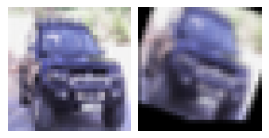
\includegraphics[width=0.6\textwidth]{images/deepLearning/AdversarialAttack/CIFAR10_rottran.png}
    \caption{Rotation-Translation: Original (L) `automobile', adversarial (R) `dog' from \cite{engstrom2017rotation}. {\em The original image of an `automobile' from the CIFAR-10 dataset is rotated (by at most $30^\circ$) and translated (by at most 3 pixels) results in an image that state-of-art classifier ResNet~\cite{he2016deep} classifies as `dog'.}}
    \label{fig:rottran}
\end{figure}

\subsection{Adversarial Attacks by Natural Transformations}\label{sec:naturalAdvAttacks}

Additional to the above approaches which perform adversarial attacks at a pixel level, research has been done on crafting adversarial examples by applying natural transformations.

\subsubsection{Rotation and Translation}

%Engstrom et al 
Some researchers \cite{engstrom2017rotation} argue that most existing adversarial attacking techniques generate adversarial images which appear to be human-crafted and less likely to be `natural'. It shows that DNNs are also vulnerable to some image transformations which are likely to occur in a natural setting. For example, translating or/and rotating an input image could significantly degrade the performance of a neural network classifier. Figure~\ref{fig:rottran} gives a few examples. 
%
Technically, given an allowed range of translation and rotation such as {\em $\pm3$ pixels $\times \pm 30^\circ$}, the attack in \cite{engstrom2017rotation} aims to find the minimum rotation and translation to cause a misclassification. To achieve such a purpose, in this work several ideas are explored including
\begin{itemize}
    \item a first-order iterative method using the gradient of the DNN's loss function,
    \item performing an exhaustive search by discretizing the parameter space,
    \item a worst-of-k method by randomly sampling $k$ possible parameter values and choosing the value that causes the DNN to perform the worst. 
\end{itemize}
%The experiments show that grid search performs best and can find adversarial examples for a significant number of images over   state-of-the-art classifiers.

\subsubsection{Spatially Transformed Adversarial Examples}

%Xiao et al 
Some researchers also
%Indeed an image may be translated by one pixel which would lead to a large $L_2$ distance, but the translated image would appear almost identical to a human. 
%They 
introduce
%therefore 
to produce uncontrived adversarial images via mortifying the pixel's location using spatial transformations instead of directly changing its pixel value \cite{xiao2018spatially}. The authors use the flow field to control the spatial transformations, which essentially quantifies the location displacement of a pixel to its new position. Figure~\ref{fig:stadvMNIST} gives a few examples. Using a bi-linear interpolation approach the generated adversarial example is differentiable w.r.t. the flow field, which then can be formulated as an optimisation problem to calculate the adversarial flow field.
Technically, they introduce a distance measure $L_{flow}(\cdot)$ (rather than the usual $L_p$ norm distance) to capture the local geometric distortion \cite{xiao2018spatially}. Similar to C\&W attack~\cite{CW2016}, the flow field is obtained by solving an optimisation problem in which the loss function is defined to balance between the $L_{flow}$ loss and adversarial loss.
%Comparing perceptual quality of spatially transformed adversarial images to adversarial images generated via other approaches in a quantitative manner is difficult due to the different measures used. However, 
Through human study, the attack in \cite{xiao2018spatially} demonstrates that adversarial examples based on such spatial transformation are more similar to original images in terms of human perceptibility, compared to those adversarial examples from $L_p$-norm based attacks such as FGSM~\cite{DBLP:journals/corr/GoodfellowSS14} and C\&W Attack~\cite{CW2016}.


\begin{figure}[t]
    \centering
    \begin{minipage}{0.24\textwidth}
        \centering
        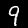
\includegraphics[width=\textwidth]{images/deepLearning/AdversarialAttack/UAN_MNIST_25sq_orig_9.png}
        \text{(a) Original:  `9'}
    \end{minipage}
    \begin{minipage}{0.24\textwidth}
            \centering
        
\includegraphics[width=\textwidth]{images/deepLearning/AdversarialAttack/UAN_MNIST_25sq_orig_9_perb_8.png}
        \text{(b) Adversarial: `8'}
    \end{minipage}
    \begin{minipage}{0.24\textwidth}
        \centering
        
\includegraphics[width=\textwidth]{images/deepLearning/AdversarialAttack/x_flow.png}
        \text{(c) x-dimension}
    \end{minipage}
    \begin{minipage}{0.24\textwidth}
            \centering
        
\includegraphics[width=\textwidth]{images/deepLearning/AdversarialAttack/y_flow.png}
        \text{(d) y-dimension}
    \end{minipage}
    \caption{Applying spatial transformation to MNIST image of a `9'~\cite{xiao2018spatially}. {\em the Image (a) on the left is the original MNIST example image of a `9', and image (b) is the spatially transformed adversarial version that a simple convolutional network \cite{papernot2018cleverhans} labels as `8'. Notice how minor the difference between the two images is - the `9' digit has been very slightly `bent' - but is sufficient for miss-classification. The flow-field that defines the spatial transformation is visualised in Image (c) (x-dimension) and Image (d) (y-dimension). The brighter areas indicate where the transformation is most intense - leftwards in the x-dimension and upwards in the y-dimension.}}
    \label{fig:stadvMNIST}
\end{figure}


\subsubsection{Towards Practical Verification of Machine Learning: The Case of Computer Vision Systems (VeriVis)}

The work in \cite{pei2017towards} introduces a verification framework, called VeriVis, to measure the robustness of DNNs on 
%`real-world' transformation functions. 
%
%Due to the often safety-critical nature of ML systems, it is imperative that DNNs can reliably classify corner-case inputs correctly. To verify this one would need to apply the system to all possible inputs - obviously not feasible. Indeed it is for exactly this reason that so much effort has been put into the generation of adversarial examples and their use for testing ML systems. However due to the extremely large domain space it is again not feasible to exhaustively generate all adversarial examples. Instead, the work in~\cite{pei2017towards} focuses on constraining a potential attacker to specific transformation functions having parameters within a specific range - for example consider the rotation function where the angle of rotation is within $\pm 10\degree $. Under these constrains, it can exhaustively test against \emph{all} transformed images. The key insight behind their approach is that ML systems work with discrete input - image pixels for example have integral coordinates taking integer values in $[0,255]$ and therefore rotation transformations having sufficiently similar angles will generate the same image. The \emph{critical} parameter domain for a given transformation and input is therefore defined as the finite subset of the parameter values that generate distinct output. This limits the domain of possible transformation functions to a finite amount (and indeed an amount which is only polynomial in the image size) thus allowing exhaustive testing. 
%
%The \textsc{VeriVis} framework specifies 
a set of twelve practical image transformations including reflection, translation, scale, shear, rotation, occlusion brightness, contrast, dilation, erosion, average smoothing, and median smoothing. Every transformation is controlled by a key parameter with a \emph{polynomial-sized} domain. Those transformations are exhaustively operated on a set of input images. Then the robustness of a neural network model can be measured.
%Thus let $\mathcal{T}(\cdot, c)$ be a transformation function parametric by $c \in C$ that transforms an input $x \in X$ to $x' = \mathcal{T}(x,c)$. A classifier $f: X \rightarrow Y$ can be thought of as \emph{Locally k-safe} for a given input $x \in X$ and transformation $\mathcal{T}(\cdot, c)$ if $f(\mathcal{T}(x,c)) \subseteq f(x, k)$ $\forall c \in C_{critical}$, where $f(x,k)$ is the set of top-k most likely predictions by $f$ for $x$, $C_{critical}$ is the critical parameter domain. A more challenging safety standard is \emph{Globally k-safe} requiring a classifier to be Locally k-safe $\forall x \in X$.
%
\textsc{VeriVis} is applied to evaluate several state-of-the-art classification models, which empirically reveals that all classifiers show a significant number of safety violations. %It is also argued that, 
%In comparison to the gradient-based adversarial techniques discussed above,
%\textsc{VeriVis} is capable of generating significantly more violations than gradient-based adversarial techniques.
%highlighting that gradient-based techniques may not be comprehensive. Furthermore the framework can be used to retrain classifiers using the found violations resulting in a more robust classifier having a greatly reduced number of safety-violations.



\subsection{Input-Agnostic Adversarial Attacks}\label{sec:inputAgnosticAdvAttacks}

A key characteristic of the above attacks lies in that an adversarial example is generated with respect to a specific input, therefore cannot be applied to other inputs. Thus some researchers show more interest in \emph{input-agnostic} adversarial perturbations.
%, and therefore may not perform adversarially when applied to another input example. %
%From the point of view of the malicious agent 

%for adversarial intent. Thus



\subsubsection{Universal Adversarial Perturbations}

The first method of input-agnostic adversarial perturbation was proposed by~\cite{moosavi2017universal}, called \emph{universal} adversarial perturbations (UAP), since UAP is able to fool a neural network on \emph{any} input images with high probability. 
%The first work on this line is proposed by Dezfooli et al \cite{moosavi2017universal}. With this approach \cite{moosavi2017universal} can generate UAPs that can fool state-of-the-art DNN classifiers with very high fooling ratios ($90\%+$ in some cases). In next, we review a few notable works in universal adversarial attacks.
%Technically, 
%Moosavi-Dezfooli et al
%\cite{moosavi2017universal} introduces UAPs and propose an algorithm for generating. The
%develope 
Let $\textbf{r}$ the the current perturbation. UAP iteratively goes through a set $D$ of inputs sampled 
%under the target 
from the input distribution $\mathcal{D}$. At the iteration for $x_i\in D$ it updates the perturbation $\textbf{r}$ as follows. First, it finds the minimal 
%(i.e. that with the smallest $L_2$-Norm) 
$\Delta \textbf{r}_i$ w.r.t. $L_2$-norm distance so that $x_i+\textbf{r}+\Delta\textbf{r}_i$ is incorrectly classified by neural network $\networks$. Then, it projects $\textbf{r} + \Delta\textbf{r}_i$ back into $L_p$-norm ball with a radius $d$ to enable that the generated perturbation is sufficiently small, i.e., let 
\begin{equation}
\begin{array}{1}
\textbf{r} = \arg\underset{\textbf{r}'}{\min} {||\textbf{r}' - (\textbf{r} + \Delta\textbf{r}_i) ||_2}\\
\text{s.t.~~} ||\textbf{r}'||_p \leq d.
\end{array}
\end{equation}
The algorithm will proceed until the empirical error of the sample set is sufficiently large, namely, no less than $1 - \delta$ for a pre-specified threshold $\delta$.


\subsubsection{Generative Adversarial Perturbations}

By training a universal adversarial network (UAN), some researchers \cite{hayes2018learning} generalised the C\&W attack in~\cite{CW2016} to generates input-agnostic adversarial perturbations. Assume that we have
%the data domain, $X$,  %classification set, %$\mathcal{Y}$, target DNN, %$g$, and 
a maximum perturbation distance $d$ and an $L_p$ norm, a UAN $\mathcal{U}_{\theta}$ randomly samples an input $z$ from a normal distribution and generates a raw perturbation $\textbf{r}$. Then it is scaled through $\textbf{w} \in [0, \frac{d}{||\textbf{r}||_p}]$ to have $\textbf{r}'=\textbf{w}\cdot \textbf{r}$. Then, the new input $\textbf{x}+\textbf{r}'$ needs to be checked with DNN $\networks$ to see if it is an adversarial example. 
%After that, $\textbf{r}'$ is added to an input $x$ and fed into $\networks$ with associated function $f$ to have %outputting 
%a prediction $f(x+\textbf{r}')$ for the adversarial image. 
The parameters $\theta$ are optimised by adopting a gradient descent method, similar to the one used by C\&W attack~\cite{CW2016}. 

%The experiments show that this UAN method generates UAPs that improve on the error rate, 1-$\delta$, from \cite{moosavi2017universal}.
%The UAN's architecture is composed of stacks of Deconvolution and Batch Normalisation layers, followed by a stack of fully-connected layers.

Later on, \cite{poursaeed2017generative} introduced a similar approach in\cite{hayes2018learning} to produce input-agnostic adversarial images. It first samples a random noise to input to UAN, and the output then is resized to meet an $L_p$ constraint which is further added to input data, clipped, and then is used to train a classifier. This method is different to~\cite{hayes2018learning} in two aspects. Firstly, it explores two UAN architectures including U-Net \cite{ronneberger2015u} and ResNet Generator \cite{johnson2016perceptual}, and concludes ResNet Generator works better in the majority of the cases. 
%The ResNet Generator architecture was  introduced 
%\cite{johnson2016perceptual} 
%for the task of \emph{image-transformation}, where the network outputs an image that has been transformed from the original input - typical transformations include colourisation, denoising or super-resolution. The architecture comprises of both up-sampling (deconvolution) and down-sampling (convolution) in residual blocks with batch normalisation and ReLU activation.
% 
Secondly, this work also trained a UAN by adopting several different classifiers, thus the proposed UAP can explicitly fool multiple classifiers, which is obtained by the below loss function:
%
\begin{equation}
    l_{multi-fool}(\lambda) = \lambda_1 \cdot l_{fool_1} + \dots + \lambda_m \cdot l_{fool_m}
\end{equation}
where $l_{fool_i}$ denotes the adversarial loss for classifier $i$, $m$ is the number of the classifiers, and $\lambda_i$ is the weight to indicate the difficulty of fooling classifier $i$.



\subsection{Practice}

%[xiaowei: here we need a code piece to do FGSM and PGD style attack on convolutional neural networks ]

First, we setup hyper-parameters (e.g., epsilon, steps, step size), device (e.g., CPU or GPU), and load training dataset (MNIST). Note that for FGSM: num-steps = 1 and  step-size = 0.031; for PGD-20: num-steps = 20 and step-size = 0.003.  
\begin{lstlisting}[language=Python]
import torch
import torch.nn as nn
import torch.nn.functional as F
import torch.optim as optim
from torchvision import datasets, transforms
import argparse
import time
import os
from torch.autograd import Variable

# Setup training parameters
parser = argparse.ArgumentParser(description='PyTorch MNIST Training')
parser.add_argument('--batch-size', type=int, default=128, metavar='N',
                    help='input batch size for training (default: 128)')
parser.add_argument('--test-batch-size', type=int, default=128, metavar='N',
                    help='input batch size for testing (default: 128)')
parser.add_argument('--lr', type=float, default=0.01, metavar='LR',
                    help='learning rate')
parser.add_argument('--no-cuda', action='store_true', default=False,
                    help='disables CUDA training')
parser.add_argument('--seed', type=int, default=1, metavar='S',
                    help='random seed (default: 1)')
parser.add_argument('--model-dir', default='./model-mnist-cnn',
                    help='directory of model for saving checkpoint')
parser.add_argument('--random', default=True,
                    help='random initialization for PGD')


# FGSM: num-steps:1 step-size:0.031   PGD-20: num-steps:20 step-size:0.003  
parser.add_argument('--epsilon', default=0.031,
                    help='perturbation')
parser.add_argument('--num-steps', default=1,
                    help='perturb number of steps, FGSM: 1, PGD-20: 20')
parser.add_argument('--step-size', default=0.031,
                    help='perturb step size, FGSM: 0.031, PGD-20: 0.003')

args = parser.parse_args(args=[]) 

if not os.path.exists(args.model_dir):
    os.makedirs(args.model_dir)
        
# Judge cuda is available or not
use_cuda = not args.no_cuda and torch.cuda.is_available()
#device = torch.device("cuda" if use_cuda else "cpu")
device = torch.device("cpu")

torch.manual_seed(args.seed)
kwargs = {'num_workers': 1, 'pin_memory': True} if use_cuda else {}

# Setup data loader
transform=transforms.Compose([
        transforms.ToTensor(),
        transforms.Normalize((0.1307,), (0.3081,))
        ])
trainset = datasets.MNIST('../data', train=True, download=True,
                   transform=transform)
testset = datasets.MNIST('../data', train=False,
                   transform=transform)
train_loader = torch.utils.data.DataLoader(trainset,batch_size=args.batch_size, shuffle=True,**kwargs)
test_loader = torch.utils.data.DataLoader(testset,batch_size=args.test_batch_size, shuffle=False, **kwargs)
\end{lstlisting}



\begin{lstlisting}[language=Python]
# Define CNN
class Net(nn.Module):
    def __init__(self):
        super(Net, self).__init__()
        # in_channels:1  out_channels:32  kernel_size:3  stride:1
        self.conv1 = nn.Conv2d(1, 32, 3, 1)
        # in_channels:32  out_channels:64  kernel_size:3  stride:1
        self.conv2 = nn.Conv2d(32, 64, 3, 1)
        self.fc1 = nn.Linear(9216, 128)
        self.fc2 = nn.Linear(128, 10)

    def forward(self, x):
        x = self.conv1(x)
        x = F.relu(x)
        x = self.conv2(x)
        x = F.relu(x)
        x = F.max_pool2d(x, 2)
        x = torch.flatten(x, 1)
        x = self.fc1(x)
        x = F.relu(x)
        x = self.fc2(x)
        output = F.log_softmax(x, dim=1)
        return output
\end{lstlisting}


Then we define the function for FGSM/PGD attack.
\begin{lstlisting}[language=Python]
def _pgd_whitebox(model,
                  X,
                  y,
                  epsilon=args.epsilon,
                  num_steps=args.num_steps,
                  step_size=args.step_size):
    out = model(X)
    err = (out.data.max(1)[1] != y.data).float().sum()
    X_pgd = Variable(X.data, requires_grad=True)
    if args.random:
        random_noise = torch.FloatTensor(*X_pgd.shape).uniform_(-epsilon, epsilon).to(device)
        X_pgd = Variable(X_pgd.data + random_noise, requires_grad=True)

    for _ in range(num_steps):
        opt = optim.SGD([X_pgd], lr=1e-3)
        opt.zero_grad()

        with torch.enable_grad():
            loss = nn.CrossEntropyLoss()(model(X_pgd), y)
        loss.backward()
        eta = step_size * X_pgd.grad.data.sign()
        X_pgd = Variable(X_pgd.data + eta, requires_grad=True)
        eta = torch.clamp(X_pgd.data - X.data, -epsilon, epsilon)
        X_pgd = Variable(X.data + eta, requires_grad=True)
        X_pgd = Variable(torch.clamp(X_pgd, 0, 1.0), requires_grad=True)
    err_pgd = (model(X_pgd).data.max(1)[1] != y.data).float().sum()
    return err, err_pgd

def eval_adv_test_whitebox(model, device, test_loader):
    # Ealuate model by white-box attack
    model.eval()
    robust_err_total = 0
    natural_err_total = 0

    for data, target in test_loader:
        data, target = data.to(device), target.to(device)
        # fgsm/pgd attack
        X, y = Variable(data, requires_grad=True), Variable(target)
        err_natural, err_robust = _pgd_whitebox(model, X, y)
        robust_err_total += err_robust
        natural_err_total += err_natural
    print('natural_accuracy: {:.2f}%'.format(0.01 * (10000-natural_err_total)))
    print('robust_accuracy: : {:.2f}%'.format(0.01 * (10000-robust_err_total)))
\end{lstlisting}


Finally, we load and attack the model.
\begin{lstlisting}[language=Python]
def main():
    model = Net().to(device)
    model.load_state_dict(torch.load(os.path.join(args.model_dir, 'final_model.pt')))
    eval_adv_test_whitebox(model, device, test_loader)
if __name__ == '__main__':
    main()
\end{lstlisting}














%\newpage
\section{Poisoning Attack}\label{sec:poisoningattackdeeplearning}

As defined in Section~\ref{sec:poisoningattackdefinition}, poisoning attack is to find a set of poisoning instances to add into the training dataset, so that the resulting trained machine learning model will perform in a wrong way according to what is required by the attacker.   
We consider both heuristic-based approaches, which generate poisoning samples with various heuristics from a set of base samples, and an alternating optimisation approach, which not only finds poisoning samples with heuristics but also continuously refines the obtained poisoning samples. 

\subsection{Heuristic Method}

For heuristic approaches, we assume there is a set $\textbf{X}_b$ of base samples. The objective is to compute another set $\textbf{X}_p$ of poisoning samples such that $\textbf{X}_p$ and $\textbf{X}_b$ are close and a target input $\textbf{x}_{adv}$ is classified as $y_{adv}$. Let $g_{\text{FE}}$ be a feature extraction function that maps every sample into a vector of features. Practically, $g_{\text{FE}}$ can be a neural network or part of a neural network, as discussed in Section~\ref{sec:representationlearning}.  The heuristic methods are discussed in \cite{10.5555/3327345.3327509,pmlr-v97-zhu19a,DBLP:conf/aaai/SahaSP20}.

\subsection*{Feature Collision} Feature collision is to synthesise one poisoning sample $\textbf{x}_{p}^{(i)}\in \textbf{X}_p$ from every base sample $\textbf{x}_{b}^{(i)}\in \textbf{X}_b$ by adding perturbation. Formally,  
\begin{equation}
    \textbf{x}_{p}^{(i)} \defequal \argmin_{\textbf{x}} ||g_{\text{FE}}(\textbf{x})-g_{\text{FE}}(\textbf{x}_{adv})||_2^2 + \beta ||\textbf{x} - \textbf{x}_{b}^{(i)}||_2^2
\end{equation}
where $\beta$ is a tunable hyper-parameter to balance between two objectives. Intuitively, it requires not only the similarity between $\textbf{x}_{p}^{(i)}$ and $\textbf{x}_{b}^{(i)}$ but also the similarity of feature representations between $\textbf{x}_{p}^{(i)}$ and the target sample $\textbf{x}_{adv}$. 

\subsection*{Convex Polytope} Instead of requiring the alignment of every poisoning sample's feature representation with that of target sample, it is also possible to synthesise the entire set  $\textbf{X}_p$ in a single round by requiring that $g_{\text{FE}}(\textbf{x}_{adv})$ aligns with a convex combination of $g_{\text{FE}}(\textbf{x}_{p}^{(i)})$. Formally, 
\begin{equation}
\begin{array}{rl}
    \textbf{X}_{p} \defequal & \displaystyle  \argmin_{c_i,\textbf{x}_p^{(i)},i=1..|X_p|} ||g(\textbf{x}_{adv})-\sum_{i=1}^{|\textbf{X}_p|}c_jg(\textbf{x}_p^{(i)})||_2^2\\
    s.t. & \displaystyle  \sum_{i=1}^{|\textbf{X}_p|} c_i=1 \\
    & \forall 1\leq i\leq |\textbf{X}_p|: c_i > 0 \\
    & \forall 1\leq i\leq |\textbf{X}_p|: ||\textbf{x}_p^{(i)} - \textbf{x}_{b}^{(i)}||_\infty \leq \epsilon
\end{array}
\end{equation}
where $\sum_{i=1}^{|\textbf{X}_p|}c_jg(\textbf{x}_p^{(i)})$ is a convex combination of $g_{\text{FE}}(\textbf{x}_{p}^{(i)})$ such that the coefficients $\{c_j~|~j=1..|\textbf{X}_p|\}$ are positive and form a probability distribution (c.f. the first two constraints). Also, we have the third constraint which ensures that the poisoning samples are close to their respective base samples.   

In the following, we have two heuristic approaches for backdoor attacks. Different from the poisoning attack, we do not have a target sample $\textbf{x}_{adv}$, but have a trigger/patch which will be added to the input instances. 

\subsection*{Hidden Trigger Backdoor} Hidden trigger backdoor is similar with Feature Collision, except that the alignment of feature representation is not between $\textbf{x}_{p}^{(i)}$ and the target sample $\textbf{x}_{adv}$, but between $\textbf{x}_{p}^{(i)}$ and a patched training image from the target 
class $y_{adv}$. Formally, 
\begin{equation}
    \textbf{x}_{p}^{(i)} = \argmin_{\textbf{x}} ||g_{\text{FE}}(\textbf{x})-g_{\text{FE}}(\tilde{\textbf{x}}_{adv}^{i})||_2^2 + \beta ||\textbf{x} - \textbf{x}_{b}^{(i)}||_2^2
\end{equation}
where $\tilde{\textbf{x}}_{adv}^{i}$ is patched training image from the target 
class $y_{adv}$. 

\subsection*{Clean Label Backdoor} Clean label backdoor proceeds in two steps. First, it generates an adversarial example $\tilde{\textbf{x}}_{adv}^{i}$ for each base sample. Second, it constructs ${\textbf{x}}_{adv}^{i}$ by adding a patch to $\tilde{\textbf{x}}_{adv}^{i}$. 


\subsection{An Alternating Optimisation Method}

As discussed in Section~\ref{sec:poisoningattackdefinition}, the data poisoning attack is a bi-level optimisation problem, which cannot be solved in a tractable way when the objective functions $\mathcal{L}_{adv}$ and $\mathcal{L}_{train}$ are non-convex. Algorithm~\ref{alg:datapoisoningalgorithm} presents an algorithm that solves the problem in an alternating optimisation way. Another method to solve the bi-level optimisation is discussed in \cite{236234}. 

\begin{algorithm}[!htbp]
\SetAlgoLined
i $\leftarrow$ 0\\
$\textbf{X}_{p}^i \leftarrow \textbf{X}_{p}$ \\ 
$\textbf{W}^i$ $\leftarrow$ $\argmin_{\textbf{W}}\mathcal{L}_{train}(\textbf{X}\cup \textbf{X}_{p}^i,\textbf{y};\textbf{W})$, where $\textbf{y}$ includes labels for both $\textbf{X}$ and $ \textbf{X}_{p}^i$ \\
$l^{i}\leftarrow \mathcal{L}_{adv}(\textbf{x}_{adv},y_{adv};\textbf{W}^i)$ \\
\Repeat{
$l^{i}-l^{i-1}< \epsilon$ 
}{
$\textbf{X}_{p}^{i+1}\leftarrow \emptyset$\\
\For{$c = 1... |X_p|$}{
$\textbf{x}_c^{i+1} \leftarrow line\_search(\textbf{x}_c^i, \nabla_{\textbf{x}_c}\mathcal{L}_{adv}(\textbf{x}_{adv},y_{adv};\textbf{W}^{i}))$\\
$\textbf{X}_{p}^{i+1}\leftarrow \textbf{X}_{p}^{i+1} \cup \{\textbf{x}_c^{i+1}\}$
}
$\textbf{W}^{i+1} \leftarrow \argmin_{\textbf{W}}\mathcal{L}_{train}(\textbf{X}\cup \textbf{X}_{p}^{i+1},\textbf{y};\textbf{W}^i)$ \\
$l^{i+1}\leftarrow \mathcal{L}_{adv}(\textbf{x}_{adv},y_{adv};\textbf{W}^{i+1})$\\
$i \leftarrow i+1$
}
\Return the final $\textbf{X}_p^i$
 \caption{$\functionname{PoisoningAttack}(\textbf{x}_{adv},y_{adv},\textbf{X}_p,\textbf{X},\mathcal{L}_{adv},\mathcal{L}_{train}, \epsilon)$, where $\textbf{x}_{adv}$ is the target input, $y_{adv}$ is the target label, $\textbf{X}_p$ is a set of initial poisoning samples, $\textbf{X}$ is the training dataset, $\mathcal{L}_{adv}(\textbf{x}_{adv},y_{adv};\textbf{W})$ is a function to measure the accuracy of predicting $\textbf{x}_{adv}$ as $y_{adv}$ with a neural network whose parameters are $\textbf{W}$,  $\mathcal{L}_{train}(\textbf{X},\textbf{y})$ is the standard training loss function, and $\epsilon>0$ is a threshold that will be used to determine the convergence. }
 \label{alg:datapoisoningalgorithm}
\end{algorithm}

It repeats by first conducting a line search over the gradient $\nabla_{\textbf{x}_c}\mathcal{L}_{adv}(\textbf{x}_{adv},y_{adv};\textbf{W}^{i})$ for all candidate samples $\textbf{x}_c$ in $\textbf{X}_p$ (Line 7-10), and then conducting a standard training over the updated $\textbf{X}\cup\textbf{X}_p$ (Line 11). The algorithm terminates when the loss over the target input converges with respect to a pre-specified threshold $\epsilon$ (Line 14). Finally, it returns the set of updated poisoning samples (Line 15). 

According to the above discussion, the key difficulty is on the computation of  \begin{equation}
    \nabla_{\textbf{x}_c}\mathcal{L}_{adv}(\textbf{x}_{adv},y_{adv};\textbf{W}^{i})
\end{equation}
which depends not only on the input $\textbf{x}_c$ but also on the weight $\textbf{W}^i$. Therefore, we can apply the chain rule and get 
\begin{equation}
    \nabla_{\textbf{x}_c}\mathcal{L}_{adv}=\nabla_{\textbf{x}_c}\textbf{W}^T \cdot \nabla_{\textbf{W}} \mathcal{L}_{adv}
\end{equation}
where we have the weight $\textbf{W}$ depends on $\textbf{x}_c$. 

It is noted that $\nabla_{\textbf{W}} \mathcal{L}_{adv}$ can be obtained through the neural network $f_{\textbf{W}}$ over the loss $\mathcal{L}_{adv}$. In the following, we explain how to compute $\nabla_{\textbf{x}_c}\textbf{W}^T$. To do so, we require that $\nabla_{\textbf{W}}\mathcal{L}_{train}(\textbf{X}\cup \textbf{X}_p,\textbf{y}; \textbf{W})=0$, according to the Karush-Kuhn-Tucker (KKT) equilibrium conditions, and further such conditions to remain valid while updating $\textbf{x}_c$, i.e., 
\begin{equation}
    \nabla_{\textbf{x}_c}(\nabla_{\textbf{W}}\mathcal{L}_{train}(\textbf{X}\cup \textbf{X}_p,\textbf{y}; \textbf{W})) = 0
\end{equation}
Through the application of chain rule on the above equation, we have 
\begin{equation}
    \nabla_{\textbf{x}_c}\nabla_{\textbf{W}}\mathcal{L}_{train} + \nabla_{\textbf{x}_c}\textbf{W}^T\cdot \nabla_{\textbf{W}}^2 \mathcal{L}_{train} = 0
\end{equation}
Therefore, we have
\begin{equation}
    \nabla_{\textbf{x}_c}\textbf{W}^T=-\nabla_{\textbf{x}_c}\nabla_{\textbf{W}}\mathcal{L}_{train}(\nabla_{\textbf{W}}^2 \mathcal{L}_{train})^{-1}
\end{equation}
where $\nabla_{\textbf{W}}\mathcal{L}_{train}$ is obtained from the neural network $f_{\textbf{W}}$ over the loss $\mathcal{L}_{train}$. 






%\newpage
\section{Model Stealing}\label{sec:modelstealingDL}

As described in Section~\ref{sec:modelstealingdefinition}, one of the typical model stealing attacks is to construct another model $f_{surrogate}$ that is \emph{functionally equivalent} to the victim model $f_{victim}$. %Unlike the setting in Section~\ref{sec:modelstealinglinearregression} where we require that the parameters in $f'$ are as close as those in $f$, we expect the  
%
We assume the black-box knowledge to the victim model, which is realistic for MLaaS applications. Specifically, for a given instance, only the output probability vector is available, or more restrictively, only the predictive label is available.   
%


For an attack, most existing methods take three steps to construct $f_{surrogate}$: \begin{enumerate}
    \item First, we build an architecture, and train an initial model $f_{surrogate}$ from easily accessible data such as randomly sampled data or public data. 
    \item Second, we synthesise further instances $\textbf{X}_{syn}$ that are on the data distribution of the victim model. 
    \item Third, we update the model $f_{surrogate}$ with the new training instances $\textbf{X}_{syn}$. 
\end{enumerate}
Moreover, considering that a single execution of the above steps might not achieve the best result, it is often that the last two steps are repeated until a pre-specified termination condition is satisfied. 

In the following, we first present a simple iterative algorithm, and then discuss alternative implementations to the individual steps. 

\subsection*{An Iterative Algorithm}

In this section, we suggest a simple, iterative algorithm that learns the model $f_{surrogate}$ gradually until convergence. The algorithm is presented in Algorithm~\ref{alg:modelstealingalgorithm}. We take the cross-entropy loss, $\mathcal{L}_{CE}$, as the training loss, but the algorithm can be extended to work with other loss functions. 

\begin{algorithm}[!htbp]
\SetAlgoLined
randomly sample a dataset $\textbf{X}_{syn}$ \\
$f_{surrogate} \leftarrow \displaystyle \argmin_{f} \sum_{\textbf{x}\in \textbf{X}_{syn}} \mathcal{L}_{CE}(f(\textbf{x}),f_{victim}(\textbf{x}))$\\
\While{
 $\displaystyle \frac{1}{|\textbf{X}_{syn}|}\sum_{\textbf{x}\in \textbf{X}_{syn}} \mathcal{L}_{CE}(f_{surrogate}(\textbf{x}),f_{victim}(\textbf{x})) \geq  \epsilon$ 
}{
$i \leftarrow 0$\\
$\textbf{X}_{syn}=\emptyset$ \\
\Repeat{i>n}{
sample a vector $\textbf{y}$ as the output prediction of a candidate input \\
$\displaystyle \textbf{x} \leftarrow \argmin_{\textbf{x}} \mathcal{L}_{CE}(f_{surrogate}(\textbf{x}),\textbf{y})$\\
$\textbf{X}_{syn} \leftarrow \textbf{X}_{syn} \cup \{\textbf{x}\}$\\
$i \leftarrow i + 1$ \\
}
$f_{surrogate} \leftarrow \displaystyle \argmin_{f} \sum_{\textbf{x}\in \textbf{X}_{syn}} \mathcal{L}_{CE}(f(\textbf{x}),f_{victim}(\textbf{x}))$\\
}
\Return $f_{surrogate}$
 \caption{$\functionname{ModelStealingAttack}(f_{victim},\epsilon,n)$, where $f_{victim}$ is the victim model that the user can access/query,  $\epsilon>0$ is a threshold that will be used to determine the convergence, and $n$ is the number of samples in the synthesised dataset. }
 \label{alg:modelstealingalgorithm}
\end{algorithm}

The algorithm proceeds by first randomly selecting a synthetic dataset $\textbf{X}_{syn}$ (Line 1) to train a surrogate model $f_{surrogate}$ (Line 2). Then, these two objects, $\textbf{X}_{syn}$ and $f_{surrogate}$,  are iteratively updated until the difference between $f_{surrogate}$ and $f_{victim}$ is smaller than the threshold $\epsilon$ (Line 3). The iterative update is conducted by synthesising samples one by one for $\textbf{X}_{syn}$ (Line 6-11). For every sample, its synthesis process proceeds by first randomly sampling a label (represented as a vector of probability values $\textbf{y}$) (Line 7), and then according to the label $\textbf{y}$ finding an instance $\textbf{x}$ with the minimum loss on the  surrogate model $f_{surrogate}$ (Line 8). 

\subsection*{Initiating Surrogate Model}

The initial training data can be, as in Algorithm~\ref{alg:modelstealingalgorithm}, a set of instances randomly sampled from the victim model. Besides, for MLaaS, it is often useful to consider public datasets such as in \cite{DBLP:conf/cvpr/OrekondySF19,DBLP:conf/aaai/PalGSKSG20}. 
For the initial model, it can start from a self-constructed architecture with randomised weights, such as in \cite{practical-black-box}, but can also start from pre-trained models from model zoos, such as Caffe Model Zoo \cite{jia2014caffe}. 

\subsection*{Synthesising Further Instances}

Usually, the training dataset for the initial surrogate model is much smaller than the victim model's training dataset, and for this reason, the initial model is not close enough to the victim model. Therefore, it is desirable to actively synthesise more instances for the update of the model. There are different approaches on how to get the new instances, including from public dataset \cite{DBLP:conf/cvpr/OrekondySF19,DBLP:conf/aaai/PalGSKSG20}, from adversarial examples \cite{practical-black-box,DBLP:conf/ndss/YuYZTHJ20}, and from data distribution of the victim model \cite{DBLP:conf/ijcai/GongCYMW21}. 


\subsection*{Updating Surrogate Model}

The update can be done by minimising the difference between $f_{surrogate}$ and $f_{victim}$ over the newly synthesised data instances, as shown in Line 12 of Algorithm~\ref{alg:modelstealingalgorithm}. We can also use a similar condition as the termination condition of the iterative process, as shown in Line 3 of Algorithm~\ref{alg:modelstealingalgorithm}. 



%\newpage
\section{Membership Inference}\label{sec:membershipInferenceDL}

As described in Section~\ref{sec:membershipinferencedefinition}, membership inference is to determine if an input $\textbf{x}$ is in the training dataset $D_{train}$ of a machine learning model $f$. 
In the following, we consider two classes of attack methods: metric-based methods and binary classifier based methods. While these methods may have different formalism and performance, all of them are based on the fact that the machine learning model $f$ has different behaviour on training data and test data. The behavioural difference is exhibited through e.g., prediction probability, loss, and hidden activations.   

\subsection{Metric Based Method}

Metric based method proceeds by first calculating a metric $M$ and then determining the membership of $\textbf{x}$ by comparing the value of the metric with a pre-specified threshold. According to the knowledge available to the attacker, there are different metrics as follows. 

\subsection*{Prediction Label Metric} 

Recall that $C$ is the set of classes and $y$ is the ground-truth label of $\textbf{x}$, we have 

\begin{equation}
    M_{label}(\textbf{x}) = \mathbbm{1}(\argmax_{c\in C} f(\textbf{x})(c) = y )
\end{equation}
where $\hat{y} = \argmax_{c\in C} f(\textbf{x})(c)$ is the predictive label and $\mathbbm{1}$ is the indicator function such that 
\begin{equation}
    \mathbbm{1}(a) = \left \{
    \begin{array}{cl}
        1 &  \text{if $a$ is True} \\
        0 &  \text{otherwise}
    \end{array}
    \right.
\end{equation}
Intuitively, this metric is based on the assumption that the model $f$ generalises so badly that it can only predict correctly on the training dataset. Based on this assumption, the sample is in the training dataset if and only if the prediction made by $f$ is correct. This attack method is black-box, i.e., it requires only knowledge \textbf{K6} (Section~
\ref{sec:attackknowlege}). 

However, most machine learning algorithms -- in particular deep neural networks --  can generalise well, which renders the above metric too coarse for membership inference.  

\subsection*{Prediction Loss Metric} 

Let $\mathcal{L}$ be the training loss function and $\epsilon$ a prespecified threshold, we define 
\begin{equation}
    M_{loss}(\textbf{x}) = \mathbbm{1}(\mathcal{L}(f(\textbf{x}), y)\leq \epsilon)
\end{equation}
Intuitively, it means that the sample $\textbf{x}$ is a member of the training dataset if its prediction loss is insignificant (i.e., smaller than $\epsilon$). The rationale behind this is that, the machine learning algorithm is trained by minimising the loss of the training data, and therefore a smaller loss suggests a higher possibility that the sample is in the training dataset. Unlike $M_{label}$ which is a black-box attack, this method requires the knowledge about the training process (or more specifically, the training loss function), i.e., the attacker knowledge \textbf{K5}. 

\subsection*{Prediction Entropy Metric}  

Recall the entropy as defined in Definition~\ref{def:entropy}, we have 
\begin{equation}
    M_{loss}(\textbf{x}) = \mathbbm{1}(H(f(\textbf{x}))\leq \epsilon)
\end{equation}
where $\epsilon$ is a pre-specified threshold. This metric is based on an observation that the uncertainty of the prediction, expressed as the entropy of the prediction probability, is smaller for training data sample than test data sample. This method is black-box. 

\subsection{Binary Classifier Based Method}

While the above metric-based methods are simple and easy to compute, they might not perform well because modern machine learning algorithms can generalise well, and more importantly, the machine learning models are very complex so that their different behaviours on the test and training datasets cannot be easily differentiated with simple metrics. This has led to the below discussion on learning a binary classifier for the membership inference. 


Intuitively, Binary classifier based attack is to learn a binary classifier $f_a$, which is able to predict the membership according to the prediction probability of the victim model $f_{victim}$. Algorithm~\ref{alg:MembershipInferencealgorithm} presents a generic framework for conducting the membership inference attack. It is a black-box algorithm and therefore can be applied to any machine learning model. 

\begin{algorithm}[!htbp]
\SetAlgoLined
Synthesise datasets $\textbf{X}_{syn,train}$ and  $\textbf{X}_{syn,test}$  such that $\textbf{X}_{syn,train}\cap \textbf{X}_{syn,test}=\emptyset$ and they follow the same distributions as the training and testing datasets of $f_{victim}$, respectively. 
%For example,  $\textbf{X}_{syn,train}=\{(\textbf{x}_1,f_{victim}(\textbf{x}_1)),...,(\textbf{x}_n,f_{victim}(\textbf{x}_n))\}$.  
\\
Construct a function $f_g: \real^{m} \rightarrow (\real^k,\{0,1\})$ that maps instances in $\textbf{X}_{syn,train}$ and  $\textbf{X}_{syn,test}$ to pairs of (probability  distribution, Binary value) \\
Train a Binary classifier $f_a: \real^k \rightarrow \{0,1\}$ that maps probability distributions to binary values by using the dataset $f_g(\textbf{X}_{syn,train})\cup f_g(\textbf{X}_{syn,test})$. \\
\Return $f_{a}\cdot f_{victim} : \real^{m} \rightarrow \{0,1\} $, which maps any sample $\textbf{x}$ to a binary value indicating whether $\textbf{x}$ is in the training dataset of $f_{victim}$.
 \caption{$\functionname{MembershipInferenceAttack}(f_{victim},m,k)$, where $f_{victim}$ is the original model that the user can access/query, $m$ is the number of input features, and $k$ is the number of classes. }
 \label{alg:MembershipInferencealgorithm}
\end{algorithm}

The algorithm takes three steps to train a binary classifier $f_a$, as discussed in the following. 
%
%\subsection*{Synthesising datasets $\textbf{X}_{syn,train}$ and $\textbf{X}_{syn,test}$} 
%
The first step is to synthesise datasets $\textbf{X}_{syn,train}$ and $\textbf{X}_{syn,test}$ that are of the same distribution as the training and test dataset of $f_{victim}$, respectively. This can be obtained with e.g., the iterative process as in Line 6-11 of Algorithm~\ref{alg:modelstealingalgorithm}. But other algorithms may also apply, for example. we can first learn a distribution from the training dataset with e.g., a generative model, and then sample dataset $\textbf{X}_{syn,train}$ from the learned distribution.  

%\subsection*{Constructing function $f_g$} 
The second step is to construct a function $f_g$ over the datasets $\textbf{X}_{syn_train}$ and $\textbf{X}_{syn,test}$. 
%partition the dataset $\textbf{X}_{syn}$ into $\textbf{X}_{syn, train}$ and $\textbf{X}_{syn, test}$, and 
This is done by first using $\textbf{X}_{syn, train}$ to train a surrogate model $f_{surrogate}$, and then letting 
\begin{equation}
    f_g(\textbf{x}) = \left \{
      \begin{array}{cl}
         (f_{surrogate}(\textbf{x}),1)  &     \text{if } \textbf{x}\in \textbf{X}_{syn, train},\\
         (f_{surrogate}(\textbf{x}),0)  &      \text{if } \textbf{x}\in \textbf{X}_{syn, test}
      \end{array}
    \right.
\end{equation} 

%\subsection*{Training Binary classifier $f_a$}

The third step is to train a Binary classifier $f_a$. 
From $f_g$ and $\textbf{X}_{syn}=\textbf{X}_{syn,train}\cup \textbf{X}_{syn,test}$, we have a dataset $f_g(\textbf{X}_{syn})$. Then, the Binary classifier $f_a$ can be obtained by using $f_g(\textbf{X}_{syn})$ as the training dataset on any machine learning model. 



\subsection*{Predicting whether new sample $\textbf{x}$ is in the training dataset of $f_{victim}$} If $f_a(f_{victim}(\textbf{x}))=0$ then it is predicted that $\textbf{x}$ is not in the training dataset. However, if $f_a(f_{victim}(\textbf{x}))=1$ then it is predicted that $\textbf{x}$ is in the training dataset. 

\subsection*{Enhancement of $f_a$ through Ensemble Method}

%We remark that, the 
The computation of $f_a$ can be improved if we take ensemble method. That is, we can have a set of classifiers $f_{a,1},...,f_{a,k}$ with Algorithm~\ref{alg:MembershipInferencealgorithm} and then the prediction on an input $\textbf{x}$ is done through a voting mechanism over these classifiers. Alternatively, we can repeat the first two steps to have a set of datasets $f_{g,1}(\textbf{X}_{syn,1}), ..., f_{g,k}(\textbf{X}_{syn,k})$, and then train a Binary classifier $f_a$ over the joint dataset $f_{g,1}(\textbf{X}_{syn,1})\cup ...\cup f_{g,k}(\textbf{X}_{syn,k})$. 


\subsection*{White-box attack}

If the attacker has more knowledge of the model $f_{victim}$, we can let the surrogate models have the same structure as the victim model and then lift the first element of $f_{g}(\textbf{x})$ to include not only the prediction probability but also other information such as the latent representations of layers. In this way, the Binary classifier $f_a$ will have more input features, which will lead to more accurate membership inference. 

\subsection*{Discussion} 

The above Binary classifier based membership inference algorithm is generic and model agnostic. It works well for simple datasets, such as low-dimensional tabular datasets, but might not work well for complex datasets, such as high-resolution image datasets. This is mainly because of the creation of dataset $\textbf{X}_{syn}$. For high-dimensional datasets, the creation of a synthetic dataset that is of the same distribution as the training dataset is non-trivial, and may require a large number of samples. 

Moreover, a membership inference attack becomes easier when the original model is overfitted. Intuitively, an overfitted model ``remembers'' the training data samples in its trainable parameters, and is therefore subject to the attack. Therefore, the improvement to the generalisation -- or the reduction of generalisation error -- of the model also poses a positive impact on data privacy. Nevertheless, a more principled study on the exact relation between them is needed. 





%\newpage
\section{Model Inversion}\label{sec:modelInversionDL}

We consider the case of reconstructing an instance $\textbf{x}$ based on the predictive output probability $f(\hat{\textbf{x}})$. There are mainly two classes of attacks: optimisation based attacks and training based attacks, which we will briefly discuss below.

\subsection{Optimisation Based Method}

The basic idea is to apply gradient based search in the input domain $\mathcal{D}$ to find an instance ${\textbf{x}}$ whose predictive output probability is close to a pre-specified probability vector $f(\hat{\textbf{x}})$. Formally, it is to solve the below optimisation problem: 
\begin{equation}\label{equ:modelinversionDL1}
    \begin{array}{rl}
        \arg\min_{\textbf{x}} & \mathcal{L}(f(\textbf{x}),f(\hat{\textbf{x}})) \\
    \end{array}
\end{equation}

However,  a naive optimisation process like Equation (\ref{equ:modelinversionDL1}) tends to generate instances (such as images) that do not really resemble natural input. Therefore, for image classification tasks, some image priors have been proposed as regularisers, i.e., we may consider the following optimisation problem: 

\begin{equation}
    \begin{array}{rl}
        \arg\min_{\textbf{x}} & \mathcal{L}(f(\textbf{x}),f(\hat{\textbf{x}})) + P(\textbf{x}) \\
    \end{array}
\end{equation}
where $P(\textbf{x})$ can be e.g., the norm distance metric such as $||\textbf{x}||_2^2$ \cite{DBLP:journals/corr/SimonyanVZ13} or $||\textbf{x}||_6^6$ \cite{DBLP:conf/cvpr/MahendranV15}, or total variation \cite{DBLP:conf/cvpr/MahendranV15}
\begin{equation}
    \sum_{i,j} ((x_{i+1,j}-x_{i,j})^2+(x_{i,j+1}-x_{i,j})^2)^{\beta/2}, 
\end{equation}
or a combination of these priors \cite{DBLP:journals/corr/YosinskiCNFL15}. 

We remark that, the optimisation based approaches require explicit access to the gradient, and therefore are white-box attacks. Moreover, they need to work with individual instances, and for this reason, can be time-consuming when there are many instances to invert. 

\subsection{Training Based Method}


Instead of optimisation based approaches, we may consider training based approaches, which aim to train a model $g$ such that 
\begin{equation}
    \argmin_{g} \mathbb{E}_{\textbf{x}\in \mathcal{D}} \mathcal{L}(g(f(\textbf{x})),\textbf{x}) 
\end{equation}
where $\mathcal{L}$ is a loss function to measure the similarity of two instances, such as the $L_2$ norm distance. Intuitively, $g$ can invert the model $f$ such that the results, expressed with $g(f(\textbf{x}))$, is close to the original input instance $\textbf{x}$. 


Recall that $f:\real^{s_1}\rightarrow \real^{s_K}$. Note that, $g:\real^{s_K}\rightarrow \real^{s_1}$ is a function mapping from the output of $f$ to the input domain. Similar to the synthesis of instances as in model stealing (Chapter~\ref{sec:modelstealingDL}), the training dataset for $g$ can be obtained either from public datasets or random sampling of the model $f$. Some additional operation may be applied to the training dataset before it is used for the training of $g$ \cite{10.1145/3319535.3354261}. While the training of $g$ may take up certain resources, it can invert instances efficiently without having prior knowledge about the model $f$. 



%\newpage 
\Extrachap{Bibliographic Notes}
%\addcontentsline{toc}{chapter}{\protect\numberline{}Bibliographic Notes}%


\subsection*{Poisoning Attack} A method to solve the bi-level optimisation is discussed in \cite{236234}. The heuristic methods are discussed in \cite{10.5555/3327345.3327509,pmlr-v97-zhu19a,DBLP:conf/aaai/SahaSP20}. 

\subsection*{Model Stealing} The adaptive approach for model stealing is discussed in \cite{DBLP:conf/ijcnn/SilvaBBSO18, DBLP:conf/cvpr/OrekondySF19}

\subsection*{Membership Inference}

Metric-based methods are discussed in \cite{8429311,DBLP:conf/ndss/Salem0HBF019} and binary classifier based method is discussed in \cite{DBLP:conf/sp/ShokriSSS17}. 

%\noexercises{
\newpage 
\Extrachap{Exercises}
%\addcontentsline{toc}{chapter}{\protect\numberline{}Exercises}%

\begin{newquestion}{\textbf{1}~~}
Consider the example dataset in Example~\ref{example:tennis}, please compute the below expressions (up to 2 decimal places) \begin{itemize}
    \item $\functionname{GainRatio}(Humidity, PlayTennis)=0.16$
    \item $\functionname{GainRatio}(Temperature, PlayTennis)=0.03$
    \item $\functionname{GainRatio}(Wind, PlayTennis)=0.05$
    \item $\functionname{InfoGain}(Humidity, PlayTennis)=0.15$
    \item $\functionname{InfoGain}(Temperature, PlayTennis)=0.03$
    \item $\functionname{InfoGain}(Wind, PlayTennis)=0.05$
\end{itemize} 
\end{newquestion}

\begin{newquestion}{\textbf{2}~~}
Consider part of the \textbf{Iris} dataset in Table~\ref{tab:irisDataset}, 
\begin{table}[h!]
    \centering
    \begin{tabular}{|c||c|c|c|c||c|}
    \hline
        Index & Sepal Length & Sepal Width & Pedal Length & Pedal Width & Iris Class \\
        \hline
        1 & 5 & 3 & 1 & 0.5 & 0 \\ 
        2 & 4 & 2 & 1 & 0.5 & 0 \\ 
        3 & 4 & 3 & 1 & 0.5 & 0 \\ 
        4 & 5 & 3 & 1 & 0.5 & 0 \\ 
        5 & 4 & 3 & 1 & 0.5 & 0 \\ 
        6 & 7 & 3 & 4 & 1 & 1 \\ 
        7 & 6 & 3 & 4 & 1 & 1 \\ 
        8 & 6 & 3 & 4 & 1 & 1 \\ 
        9 & 4 & 2 & 3 & 1 & 1 \\ 
        10 & 6 & 3 & 6 & 2 & 2 \\ 
        11 & 5 & 2 & 5 & 2 & 2 \\ 
        12 & 7 & 3 & 5 & 2 & 2 \\ 
        13 & 5 & 2 & 5 & 2 & 2 \\ 
        14 & 7 & 2 & 5 & 1 & 2 \\ 
         \hline
    \end{tabular}
    \caption{Part of \textbf{Iris} dataset}
    \label{tab:irisDataset}
\end{table}
please compute the below expressions (up to 2 decimal places) \begin{itemize}
    \item $\functionname{GainRatio}(Sepal Length, Iris Class)=$
    \item $\functionname{GainRatio}(Sepal Width, Iris Class)=$
    \item $\functionname{GainRatio}(Pedal Length, Iris Class)=$
    \item $\functionname{GainRatio}(Pedal Width, Iris Class)=$
    \item $\functionname{InfoGain}(Sepal Length, Iris Class)=$
    \item $\functionname{InfoGain}(Sepal Width, Iris Class)=$
    \item $\functionname{InfoGain}(Pedal Length, Iris Class)=$
    \item $\functionname{InfoGain}(Pedal Width, Iris Class)=$

\end{itemize} 
\end{newquestion}

\begin{newquestion}{\textbf{3}~~}
Understand the basic idea of random forest by conducting research on the literature, and implement a random forest algorithm based on the decision tree algorithm to see if random forest performs better than decision tree on \textbf{Iris} dataset. 
\end{newquestion}

\begin{newquestion}{\textbf{4}~~}
Following the last newquestion, please give an adversarial attack algorithm for random forest. 
\end{newquestion}

\begin{newquestion}{\textbf{5}~~}\label{newquestion:linearregression}
Consider the four data samples in Example~\ref{example:linearregression} (also provided in Table~\ref{tab:footballplayers2}) 
\begin{table}[h!]
    \centering
    \begin{tabular}{|c|c|c|c|}
    \hline
      $X_1$   & $X_2$ & $X_3$ & $Y$ \\
      \hline
      182   & 87 & 11.3 & 325 \\
      189   & 92 & 12.3 & 344 \\
      178   & 79 & 10.6 & 350 \\
      183   & 90 & 12.7 & 320 \\
      \hline
    \end{tabular}
    \caption{A small dataset}
    \label{tab:footballplayers2}
\end{table}
and the mean square error, if we have the following two functions: 
\begin{itemize}
    \item $f_{\textbf{w}_1}=2X_1+1X_2+20X_3-330$
    \item $f_{\textbf{w}_2}=X_1-2X_2+23X_3-332$
\end{itemize}
please newanswer the following newquestions:
\begin{enumerate}
    \item which model is better for linear regression?
    \item which model is better for linear classification
 	   by considering 0-1 loss for $\textbf{y}^T=(0,1,1,0)$?
 	  \item which model is better for logistic regression for $\textbf{y}^T=(0,1,1,0)$? 
 	  \item According to the logistic regression of the first model, what is the prediction result of the first model on a new input $(181,92,12.4)$?
\end{enumerate}
\end{newquestion}
\begin{newanswer*}
(1) Because 
\begin{equation}
\begin{array}{rll}
    f_{\textbf{w}_1}(\textbf{x}_1)-y_1 = & 2*182+1*87+20*11.3-330-325 & =  22 \\
    f_{\textbf{w}_1}(\textbf{x}_2)-y_2 = & 2*189+1*92+20*12.3-330-344 & =  42 \\
    f_{\textbf{w}_1}(\textbf{x}_3)-y_3 = & 2*178+1*79+20*10.6-330-350 & =  -33 \\
    f_{\textbf{w}_1}(\textbf{x}_4)-y_4 = & 2*183+1*90+20*12.7-330-320 & =  60 \\
    
    f_{\textbf{w}_2}(\textbf{x}_1)-y_1 = & 182-2*87+23*11.3-332-325 & =  -389.1 \\
    f_{\textbf{w}_2}(\textbf{x}_2)-y_2 = & 189-2*92+23*12.3-332-344 & =  -388.1 \\
    f_{\textbf{w}_2}(\textbf{x}_3)-y_3 = & 178-2*79+23*10.6-332-350 & =  -418.2 \\
    f_{\textbf{w}_2}(\textbf{x}_4)-y_4 = & 183-2*90+23*12.7-332-320 & =  -356.9 \\
\end{array}
\end{equation} the model $f_{\textbf{w}_1}$ is better for linear regression, according to the loss function (Equation~\ref{equ:linearregression2}); 

(2) Because
\begin{equation}
\begin{array}{cc}
    step(f_{\textbf{w}_1}(\textbf{x}_1))=1\\
    step(f_{\textbf{w}_1}(\textbf{x}_2))=1\\
    step(f_{\textbf{w}_1}(\textbf{x}_3))=1\\
    step(f_{\textbf{w}_1}(\textbf{x}_4))=1\\
    step(f_{\textbf{w}_2}(\textbf{x}_1))=0\\
    step(f_{\textbf{w}_2}(\textbf{x}_2))=0\\
    step(f_{\textbf{w}_2}(\textbf{x}_3))=0\\
    step(f_{\textbf{w}_2}(\textbf{x}_4))=0\\
\end{array}
\end{equation}
we have that both models are the same, according to the loss function (Equation~\ref{equ:linearclassification2}); 

(3) Because 
\begin{equation}
\begin{array}{rcl}
    y_1*\log(\sigma(f_{\textbf{w}_1}(\textbf{x}_1)))+(1-y_1)\log((1-\sigma(f_{\textbf{w}_1}(\textbf{x}_1))))&=&-M\\
    y_2*\log(\sigma(f_{\textbf{w}_1}(\textbf{x}_2)))+(1-y_2)\log((1-\sigma(f_{\textbf{w}_1}(\textbf{x}_2))))&=&0\\
    y_3*\log(\sigma(f_{\textbf{w}_1}(\textbf{x}_3)))+(1-y_3)\log((1-\sigma(f_{\textbf{w}_1}(\textbf{x}_3))))&=&0\\
    y_4*\log(\sigma(f_{\textbf{w}_1}(\textbf{x}_4)))+(1-y_4)\log((1-\sigma(f_{\textbf{w}_1}(\textbf{x}_4))))&=&-M\\
    
    y_1*\log(\sigma(f_{\textbf{w}_2}(\textbf{x}_1)))+(1-y_1)\log((1-\sigma(f_{\textbf{w}_2}(\textbf{x}_1))))&=&0\\
    y_2*\log(\sigma(f_{\textbf{w}_2}(\textbf{x}_2)))+(1-y_2)\log((1-\sigma(f_{\textbf{w}_2}(\textbf{x}_2))))&=&-44.1\\
    y_3*\log(\sigma(f_{\textbf{w}_2}(\textbf{x}_3)))+(1-y_3)\log((1-\sigma(f_{\textbf{w}_2}(\textbf{x}_3))))&=&-68.2\\
    y_4*\log(\sigma(f_{\textbf{w}_2}(\textbf{x}_4)))+(1-y_4)\log((1-\sigma(f_{\textbf{w}_2}(\textbf{x}_4))))&=&-1.1\\
\end{array}
\end{equation}
where $M$ represents a large number, so we have  
\begin{equation}
\begin{array}{c}
\hat{L}(f_{\textbf{w}_1}) = -\frac{1}{4}(-M+0+0-M)=M/2\\
\hat{L}(f_{\textbf{w}_2}) = -\frac{1}{4}(0-44.1-68.2-1.1)=28.35
\end{array}
\end{equation}
according to Equation (\ref{equ:logisticregression3}). 
Therefore, $f_{\textbf{w}_2}$ is better. 

(4) According to Equation (\ref{equ:logisticregression2}), we have 
\begin{equation}
\begin{array}{c}
     P_{\textbf{w}_1}(y=1|\textbf{x})=\sigma(2*181+1*92+20*12.4-330)=1 \\
     P_{\textbf{w}_1}(y=0|\textbf{x})=1-\sigma(2*181+1*92+20*12.4-330)=0
\end{array}
\end{equation}
Therefore, it is predicted to 1. 
\end{newanswer*}

\begin{newquestion}{\textbf{6}~~}
Understand the basic idea of Bayesian linear regression by conducting research on the literature, and implement a Bayesian linear regression algorithm to compare its performance with linear regression. 
\end{newquestion}

\begin{newquestion}{\textbf{7}~~}
Write a program for the adversarial attack for logistic regression. 
\end{newquestion}

\begin{newquestion}{\textbf{8}~~}
Given a function $f(x)= e^x/(1+e^x)$, how many critical points? 
\end{newquestion}
\begin{newanswer*}
0
\end{newanswer*}

\begin{newquestion}{\textbf{9}~~}
Given a function $f(x_1,x_2)= 9x_1^2+3x_2+4$, how many critical points? 
\end{newquestion}
\begin{newanswer*}
0, because there is no assignment to $x_1$ and $x_2$ that can make the gradient of $f(x_1,x_2)$ equal to $0$. 
\end{newanswer*}

\begin{newquestion}{\textbf{10}~~}
Consider the dataset in Table~\ref{tab:workhours}, 
\begin{table}[h!]
    \centering
    \begin{tabular}{|c|c|c|}
    \hline
       Gender  & HrsWorked & Wealthy? \\
       \hline
       F  & 39 & Y \\
       F  & 45 & N \\
       M  & 35 & N \\
       M  & 43 & N \\
       F  & 32 & Y \\
       F  & 47 & Y \\
       M  & 34 & Y \\
       \hline
    \end{tabular}
    \caption{A small dataset}
    \label{tab:workhours}
\end{table}
please newanswer the following newquestion:
\begin{itemize}
    \item $P(Wealthy=Y) = 4/7 $
    \item $P(Wealthy=N)= 3/7 $
    \item $P(Gender=F | Wealthy = Y) = 3/4$
    \item $P(Gender=M | Wealthy = Y) = 1/4 $
    \item $P(HrsWorked > 40.5 | Wealthy = Y) = 1/4$
    \item $P(HrsWorked < 40.5 | Wealthy = Y) = 3/4$
    \item $P(Gender=F | Wealthy = N) = 1/3$
    \item $P(Gender=M | Wealthy = N) = 2/3 $
    \item $P(HrsWorked > 40.5 | Wealthy = N) = 2/3$
    \item $P(HrsWorked < 40.5 | Wealthy = N) =1/3$
\end{itemize}
Based on the above, please use 
Classify a new instance with Naive Bayes algorithm (Gender = F,  HrsWorked = 44). 
\end{newquestion}
\begin{newanswer*}
Because 
\begin{equation}
\begin{array}{l}
    P(Wealthy=Y)*P(Gender=F | Wealthy = Y)*\\
    P(HrsWorked > 40.5 | Wealthy = Y) =  3/28\\
     P(Wealthy=N)*P(Gender=F | Wealthy = N)*\\
     P(HrsWorked > 40.5 | Wealthy = n) =   2/21\\   
\end{array}
\end{equation}
we have that it will be predicted as $Wealthy=Y$ according to Equation (\ref{equ:nbes}).
\end{newanswer*}
%\newpage
%\Extrachap{Exercise}
%\addcontentsline{toc}{chapter}{\protect\numberline{}Exercise}%

\begin{newquestion}{\textbf{11}~~}
Implement the perceptron learning algorithm in Section~\ref{sec:perceptron}, and compare the obtained binary classifier with the one obtained from logistic regression. 
\end{newquestion}

\begin{newquestion}{\textbf{12}~~}
Understand how learning rate in the perceptron learning algorithm affects the learning results. Draw a curve to exhibit the change of accuracy with respect to the learning rate. 
\end{newquestion}

\begin{newquestion}{\textbf{13}~~}
Use the perceptron learning algorithm to work with the XOR dataset in Example~\ref{example:xor}, and check the accuracy. 
\end{newquestion}




\begin{newquestion}{\textbf{14}~~}
Assuming that all weights in Figure~\ref{fig:twolayerxor}, i.e., those numbers 1 and -1, need to be learned. Can you adapt the perceptron learning algorithm to learn the weights? 
\end{newquestion}


\begin{newquestion}{\textbf{15}~~}
Understand the equivalence of applying matrix expression to compute the outputs for a dataset and the computation of outputs for individual inputs. 
\end{newquestion}
%}

%\chapter{Loss Functions and Regularisation}

%%\newpage
%\section{Introduction}

Up to now, we have known that machine learning algorithms can be used to effectively learn a function $f$ from a set of input-output pairs. The function $f$ approximates the relation between two random variables $X$ and $Y$, and actually expresses the conditional probability $P_f(Y|X)$. However, in a complex, real world system, there might be more than two random variables and it is useful to not only understand the the conditional probability between random variables but also be able to infer more intriguing information from the conditional dependence relations between random variables.
It is also possible that, a complex machine learning model, such as a convolutional neural network, can be approximated by constructing the conditional dependencies between a set of random variables representing the features learned by the neural networks, see e.g., \cite{berthier2021abstraction} for an example.  Therefore, while it is agreeable that machine learning has been able to support human operators in dealing with some long-standing tasks such as object detection and recognition with accuracy and efficiency, there is still a need to infer useful knowledge from a set of conditional probabilities. 
This chapter is to explain how we may utilise probabilistic graphical model, a formalism to express conditional probabilities between random variables ($X$, $Y$, and variables for latent representations), as an abstract model for neural network. We will present the definition in Section~\ref{sec:defPGM} and then discuss the abstraction method in Section~\ref{chap:NNabstraction}. More detailed introduction to probabilistic graphical models is given in the Appendix (Chapter~\ref{chap:pgm}). 

\section{Definition of Probabilistic Graphical Models}\label{sec:defPGM}

Probabilistic graphical models are a formalism for the above purpose. They use a structure, or more specifically a graph, to represent conditional dependence relations between random variables, and use a probability table for every random variable to express the local dependence relation of the random variable. There are two major branches of graphical models, namely, Bayesian networks and Markov random fields, and in this chapter, we focus on Bayesian network. In the following, we will use (probabilistic) graphical models and Bayesian network interchangeably. 


Depending on the dependence relation of individual random variable, the probability tables in a graphical model can be a marginal probability table, which shows that the random variable does not depend on any other variables in the graph, or a conditional probability table, which represents the conditional probability distribution of the current random variable over other random variables in the graph. 

\begin{figure}[!htbp]
    \centering
    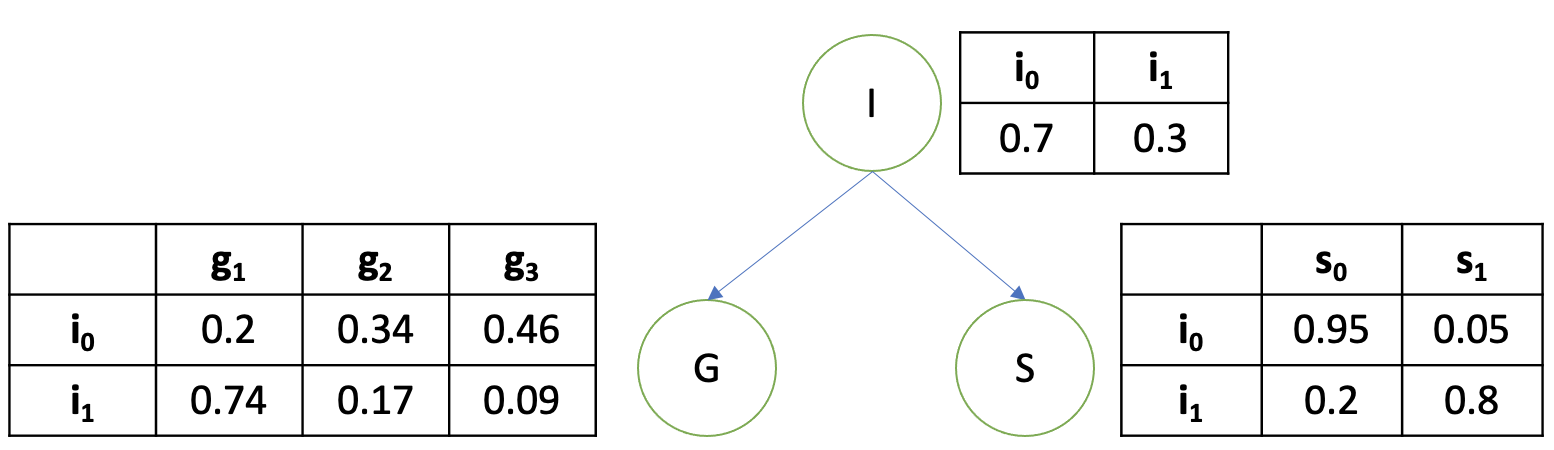
\includegraphics[width=0.7\textwidth]{images/graphical models/threeNodes.png}
    \caption{A simple graphical model of three nodes}
    \label{fig:threeNodes}
\end{figure}


Figure~\ref{fig:threeNodes} presents a simple graphical model with 3 nodes: $I, G, S$. We can see that one of the nodes $I$ has a marginal probability table while the remaining two nodes have conditional probability tables. 
Summarising, 
\begin{equation}
    \text{Probabilistic Graphical Model = Graphical Structure + Multivariate Statistics}
\end{equation}
Formally, a probabilistic graphical model $G=({\cal V},{\cal E},P)$ where ${\cal V}$ is a set of nodes, representing the random variables, ${\cal E}$ is the set of edges between nodes, and $P$ is a set of probability tables, one for each node in ${\cal V}$. 

\section*{A Running Example}

Assume that, on a self-driving car, there are two sensors, $Camera$ and $Radar$, that are used to detect pedestrian collectively. The precision of the  camera may be affected by weather conditions, such as the $Fog$ as we consider in this example. The $Radar$ may be affected by the distance of the object from the car, i.e., it can be very precise when the object is close but may become less precise when the object is $Away$. Once a pedestrian is detected and it is not away, the car will need to stop. 

%\begin{example}


\begin{figure}[!htbp]
    \centering
    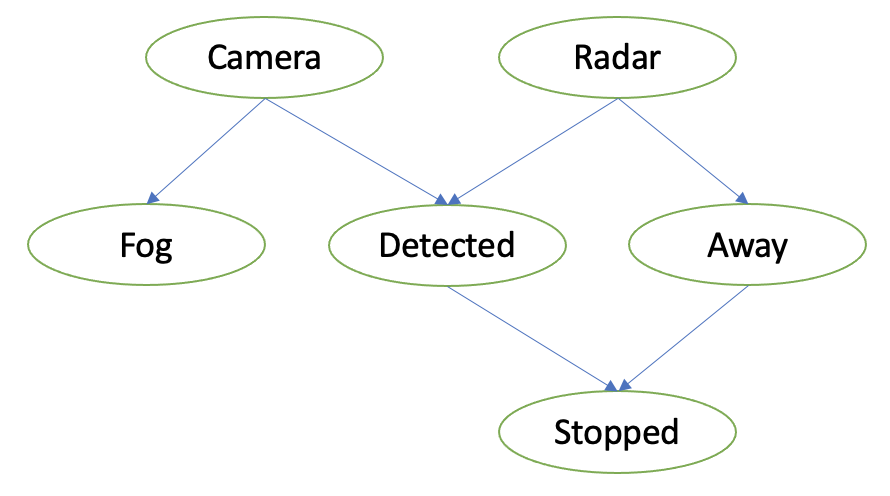
\includegraphics[width=0.6\textwidth]{images/graphical models/graphicalmodel.png}
    \caption{A simple Bayesian network for safety analysis on vehicle stopping upon pedestrian detection}
    \label{fig:graphicalmodel}
\end{figure}

Figure~\ref{fig:graphicalmodel} presents a probabilistic graphical model for this example. In the graph $G$, there are six random variables: $Camera$, $Radar$, $Fog$, $Detected$, $Away$, and $Stopped$. Every node is associated with either a marginal probability table or a conditional probability table, depending on whether they have incoming edges. The information about the probability tables are given in Figure~\ref{fig:cameratables}. For example, the nodes $Camera$ and $Radar$ do not have incoming edges, so each of them is associated with a marginal probability table. Intuitively, the two tables suggest that the probability of a pedestrian appearing in the imagery input of the camera is $0.4$, and in the signal input of the radar is $0.5$. Note that, the ``appearing'' is for ground truth (through human's eyes), not for the result of a detection system. The detection is implemented through the $Detected$ node to be explained below. 


%\end{example}


\begin{figure}[!htbp]
    \centering
    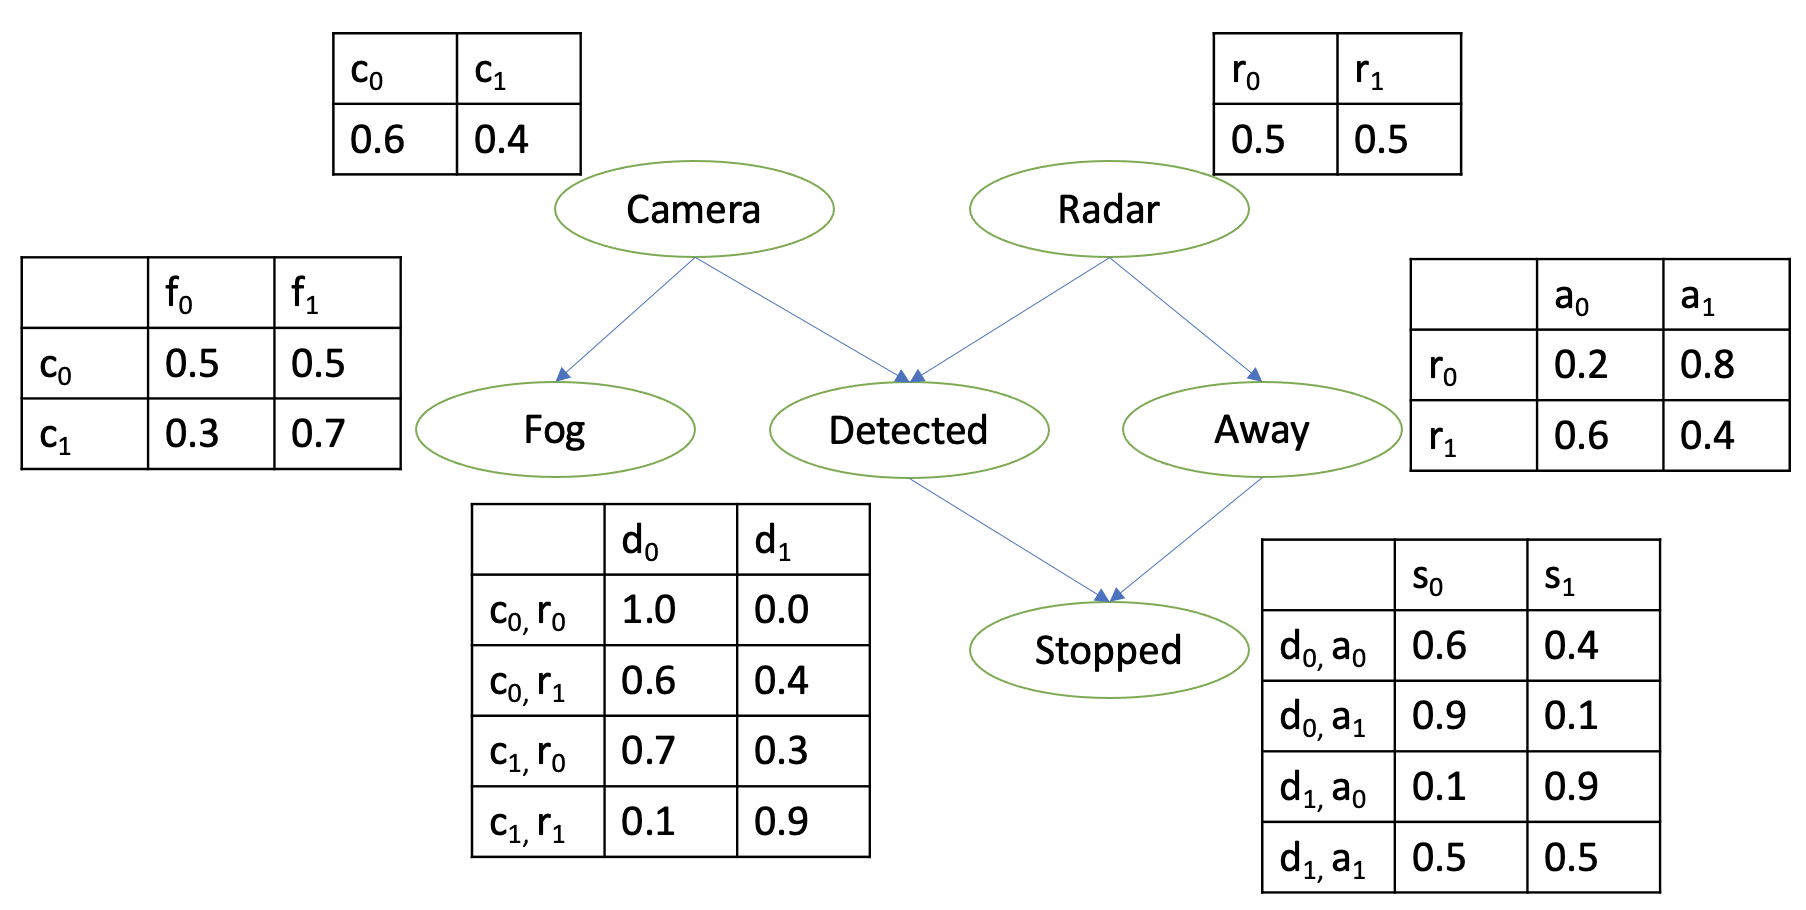
\includegraphics[width=\textwidth]{images/graphical models/cameramodel.png}
    \caption{Probabilistic table of the graphical model in Figure~\ref{fig:graphicalmodel}}
    \label{fig:cameratables}
\end{figure}


Other nodes are associated with conditional probability tables. For example, the table for $Fog$ shows that, when there is no pedestrian appearing in the imagery input, the probability of the foggy weather condition is $0.5$.  This probability is lowered when there is a pedestrian appearing in the imagery input. This is intuitive, because the foggy condition may affect the ability of camera capturing the pedestrian. Similar for the $Away$ node. When there is no pedestrian appearing in the signal input, the probability of its away from a pedestrian is $0.8$. This probability is lowered to $0.4$ when there is a pedestrian appearing in the signal input. 

The detection result is a fusion of both camera and radar's results. Note that, even if a pedestrian appears in the imagery input, it does not mean that the pedestrian can be detected (Recall the generalisation error and robustness error of deep learning). We note that, if neither of the sensors has a pedestrian appeared, no detection can be made at all. If one of the sensors has a pedestrian, there is a non-trivial chance that it can be detected. The detection becomes significantly better when both sensors captured the pedestrian. 

Finally, the decision making on whether the car should be stopped is based on both the detection result and the distance. If it is detected (i.e., $Detected = d_1$) and not far away (i.e., $Away = a_0$) then this probability is high ($0.9$). Otherwise, the probability is low ($0.1$). The lowest probability appears when no pedestrian is detected (i.e., $Detected = d_0$) and it is away (i.e., $Away = a_1$). 

\subsection*{Where does machine learning play a role?}

Machine learning can be used to generate those conditional probability tables. For example, a deep learning model can be designed and trained to get the table for $Detected$ node, i.e., classify whether a pedestrian is detected or not on both the camera input and the radar input. Similarly, other nodes such as $Fog$, $Away$, and $Stopped$ may also be implemented with a machine learning model. 







%%\newpage
%\section{Adversarial Training}



